\documentclass{beamer}

\usepackage{color, colortbl}

\mode<presentation>
{
    %\usetheme{AnnArbor}
    %\usetheme{Antibes}
    %\usetheme{Bergen}
    %\usetheme{Berkeley}
    %\usetheme{Berlin}
    %\usetheme{Boadilla}
    %\usetheme{CambridgeUS}
    %\usetheme{Copenhagen}
    %\usetheme{Darmstadt}
    %\usetheme{Dresden}
    %\usetheme{Frankfurt}
    %\usetheme{Goettingen}
    %\usetheme{Hannover}
    %\usetheme{Ilmenau}
    %\usetheme{JuanLesPins}
    %\usetheme{Luebeck}
    \usetheme{Madrid}
    %\usetheme{Malmoe}
    %\usetheme{Marburg}
    %\usetheme{Montpellier}
    %\usetheme{PaloAlto}
    %\usetheme{Rochester}
    %\usetheme{Singapore}            % maybe
    %\usetheme{Szeged}
    %\usetheme{Warsaw}
    %\setbeamercovered{transparent}
    \usecolortheme{seahorse}
}

\setbeamertemplate{footline}
{
  \leavevmode%
  \hbox{%
  \begin{beamercolorbox}[wd=.2\paperwidth,ht=2.25ex,dp=1ex,center]{author in head/foot}%
	  \usebeamerfont{author in head/foot}Martin Hru\v{s}ka
  \end{beamercolorbox}%
  \begin{beamercolorbox}[wd=.7\paperwidth,ht=2.25ex,dp=1ex,center]{title in head/foot}%
    \usebeamerfont{title in head/foot}\insertshorttitle
  \end{beamercolorbox}}%
  \begin{beamercolorbox}[wd=.1\paperwidth,ht=2.25ex,dp=1ex,center]{date in head/foot}
            \insertframenumber{} / \inserttotalframenumber 
        \end{beamercolorbox}%
  \vskip0pt%
}

\setbeamertemplate{itemize item}[square]
\setbeamertemplate{itemize subitem}[triangle]
\setbeamertemplate{itemize subsubitem}[circle]
% \setbeamertemplate{enumerate item}[square]
\setbeamertemplate{section in toc}[square]
\setbeamertemplate{navigation symbols}{}

\newenvironment{figure*}%
{\begin{figure}}
{\end{figure}}

\usepackage{adjustbox}
\usepackage{comment}
\usepackage{ucs}
\usepackage[utf8x]{inputenc}
%\usepackage{palatino}
\usepackage{color}
\usepackage{graphicx}
%\usepackage{alltt}
\usepackage{tikz}
\usepackage{subcaption}
%\usepackage{MnSymbol}
%\usepackage{wasysym}
\usepackage[nofillcomment,noend,linesnumbered,noline,oldcommands]{algorithm2e}
\usetikzlibrary{calc,matrix,backgrounds,fit,shapes,arrows}

\usetikzlibrary{arrows}
\usetikzlibrary{backgrounds}
\usetikzlibrary{calc}
\usetikzlibrary{fit}
\usetikzlibrary{decorations}
\usetikzlibrary{decorations.pathmorphing}
\usetikzlibrary{decorations.pathreplacing}

\newcommand{\hlbl}[1]{\textcolor{blue}{#1}}
\newcommand{\hlgr}[1]{\textcolor{olive!50!green}{#1}}
\newcommand{\hlrd}[1]{\textcolor{red}{#1}}
\newcommand{\hlye}[1]{\textcolor{magenta}{#1}}
\newcommand{\hcol}[1]{yellow!20!orange!20}
\newcommand{\ucol}[1]{red!50}
\newcommand{\scol}[1]{blue!40}

\newcommand{\todo}[1]{\hlbl{[TODO: #1]}} 
\newcommand{\nt}[1]{\hlgr{[NOTE: #1]}} 

\newcommand{\heaps}{\mathcal{H}}
\newcommand{\partrel}{\approx}

%%%%%%%%%%%%%%%%%%%%%%%%%%%%%%%%%%%%%%%%%%%%%%%%%%%
% \todo,remark
%%%%%%%%%%%%%%%%%%%%%%%%%%%%%%%%%%%%%%%%%%%%%%%%%%%%
\newcommand{\td}[1]{\textcolor{blue}{[#1]}} 
% \newcommand{\td}[1]{} 
\newcommand{\rem}[1]{\textcolor{green}{[NOTE: #1]}}
\newcommand{\fixme}[1]{\textcolor{red}{[FIXME: #1]}}
\newcommand{\achtung}[1]{{\centering \textcolor{red}{!!!ACHTUNG!!!\\{\centering #1}\linebreak\hfill!!!ACHTUNG!!!\\}}}
\newcommand{\drop}[1]{\textcolor{red}{#1}}
\newcommand{\chk}[1]{\textcolor{blue}{#1}}

%%%%%%%%%%%%%%%% SOA %%%%%%%%%%%%%%%%%%%%%%%%%%%%%%
\newcommand{\mw}{{-\!\!\ast}}
%%%%%%%%%%%%%%%%%%%%%%%%%%%%%%%%%%%%%%%%%%%%%%%%%%%


%%%%%%%%%%%%%%%%%%%%%%%%%%%%%%%%%%%%%%%%%%%%%%%%%%%
% radustyle comments 
%%%%%%%%%%%%%%%%%%%%%%%%%%%%%%%%%%%%%%%%%%%%%%%%%%%
\definecolor{darkgreen}{rgb}{0,0.6,0}

%\renewcommand{\td}[1]{} 
%\renewcommand{\rem}[1]{}
%\renewcommand{\fixme}[1]{}
%\renewcommand{\achtung}[1]{}
%\renewcommand{\drop}[1]{}
%\renewcommand{\chk}[1]{}

%%%%%%%%%%%%%%%%%%%%%%%%%%%%%%%
%\newcommand\figswitch[1]{Figure}%
\newcommand\figswitch[1]{#1}%
%%%%%%%%%%%%%%%%%%%%%%%%%%%%%%%%

%%%% MOVED from projekt-01.*.tex
\newcommand{\rig}[1]{\bigstar(#1)}
\newcommand{\cut}{\rhd}
\newcommand{\filter}[1]{\mathord\Phi_{#1}}
\newcommand{\cpp}{C\nolinebreak\hspace{-.03em}\raisebox{.3ex}{+}\nolinebreak\hspace{-.07em}\raisebox{.3ex}{+}}



%%%%%%%%%%%%%%%%%%%%%%%%%%%%%%%%%%%%%%%
%% Current paper
%%%%%%%%%%%%%%%%%%%%%%%%%%%%%%%%%%%%%%%
\newcommand{\lerr}{\preceq_{rr}}
\newcommand{\lera}{\preceq_{ra}}
\newcommand{\lear}{\preceq_{ar}}
\newcommand{\leaa}{\preceq_{aa}}

\newcommand{\gerr}{\succeq_{rr}}
\newcommand{\gera}{\succeq_{ra}}
\newcommand{\gear}{\succeq_{ar}}

\newcommand{\lrr}{\prec_{rr}}
\newcommand{\lra}{\prec_{ra}}
\newcommand{\lar}{\prec_{ar}}
\newcommand{\laa}{\prec_{aa}}

\newcommand{\grr}{\succ_{rr}}
\newcommand{\gra}{\succ_{ra}}
\newcommand{\gar}{\succ_{ar}}
\newcommand{\gaa}{\succ_{aa}}
\newcommand{\rank}{\sharp}
\newcommand{\rankof}[1]{\rank{#1}}
\newcommand{\ltr}[1]{\mathrel{\stackrel{\!\!#1}{\raisebox{0pt}[0.50ex][0pt]{\ensuremath{\rightarrow}}}}}
%\newcommand{\edgeof}[3]{#1\ltr{#2} #3} % please do not 
\newcommand{\edgeof}[3]{(#2,#1,#3)}  
%\newcommand{\edgeof}[3]{#1\to(#2,#3)}
\newcommand{\nset}[1]{\{1,\ldots,#1\}}
\newcommand{\partialto}{\rightharpoonup}
\newcommand{\selmapof}[1]{\text{\textsl{next\/}}_{#1}}
\newcommand{\symselof}[2]{#1_{#2}}
\newcommand{\selof}[1]{\symselof{a}{#1}}
%\newcommand{\nset}[1]{\intof 1 #1}
%\newcommand{\nset}[1]{\langle#1\rangle}
\newcommand{\constr}{\varphi}
\newcommand{\denotationof}[1]{\semof{#1}}
\newcommand{\fa}{F}
\newcommand{\ta}{A}
\newcommand{\forest}{f}
%\newcommand{\oforest}{(\forest,\fports)}
\newcommand{\tree}{t}
\newcommand{\graph}{g}
% \newcommand{\graph}{h}
\newcommand{\graphprime}{\graph'}
\newcommand{\graphprimeprime}{\graph''}
\newcommand{\hgraph}{h}
\newcommand{\fports}{\pi} %ports of a forest (aut)
\newcommand{\gports}{\phi} %ports of a graph
%\newcommand{\rrefof}[1]{\mathit{ref}(#1)}
\newcommand{\rootof}[1]{\mathit{root}(#1)}
%\newcommand{\rrlof}[1]{\mathit{rrl}(#1)}
\newcommand{\strlabof}[1]{#1^{\mathit{str}}}
\newcommand{\lang}{L}
\newcommand{\langof}[1]{\lang({#1})}
\newcommand{\flangof}[1]{\lang_f(#1)}
\newcommand{\smap}{S}
\newcommand{\node}{v}
\newcommand{\nodep}{u}
\newcommand{\nodepp}{w}
\newcommand{\nodesof}[1]{V_{#1}}
\newcommand{\datmapof}[1]{\lambda_{#1}}
\newcommand{\edge}{e}
\newcommand{\sorderof}[1]{\sqsubset_#1}
\newcommand{\sordereqof}[1]{\sqsubseteq_#1}
\newcommand{\trees}{t_1\cdots t_n}
\newcommand{\treesprime}{t_1'\cdots t_n'}
%\newcommand{\fport}{\iota}
\newcommand{\fport}{\fports}
\newcommand{\gport}{\gports}
\newcommand{\run}{\rho}
\newcommand{\runof}[1]{\run(#1)}
%\newcommand{\tas}{\bar \ta}
\newcommand{\tas}{\ta_1\cdots \ta_n}
\newcommand{\tasprime}{\ta'_1\cdots \ta'_n}
\newcommand{\tasencoded}{\encof{\ta_1} \ldots \encof{\ta_n}}
\newcommand{\tasin}[1]{\ta^{#1}_1\cdots \ta^{#1}_n}
\newcommand{\subst}[2]{[#1/#2]} %co, za co
\newcommand{\fas}{\mathbb{F}}
\newcommand{\img}{\mathit{img}}
\newcommand{\dom}{\mathit{dom}}
\newcommand{\Img}{\mathit{Img}}
\newcommand{\imgof}[1]{\mathit{img}(#1)}
\newcommand{\domof}[1]{\mathit{dom}(#1)}
\newcommand{\knot}{k}
\newcommand{\knotprime}{\knot'}
\newcommand{\knotprimeprime}{\knot''}
\newcommand{\knots}{K}
\newcommand{\knotwithjingles}{b}
\newcommand{\subgrapheq}{\trianglelefteq}
\newcommand{\subgraph}{\triangleleft}
\newcommand{\cp}{c}
\newcommand{\cpsof}[1]{\mathit{cps}(#1)}
\newcommand{\optof}[3]{\lozenge(#1,#2,#3)}
\newcommand{\join}{j}
\newcommand{\joinsof}[1]{\mathit{joins}(#1)}
\newcommand{\fork}{f}
%\newcommand{\entryof}[3]{#2\Yleft_{#1} #3}
\newcommand{\forkof}[2]{\mathit{fork}(#1,#2)}
\newcommand{\reachesin}[1]{\Longrightarrow_{#1}}
\newcommand{\edgesof}[1]{e_{#1}}
\newcommand{\edgesofnode}[2]{\edgesof{#1}(#2)}
\newcommand{\gsedgesof}[1]{\mathit{SE}(#1)}
\newcommand{\vsedgesof}[2]{\mathit{SE}(#1,#2)}
\newcommand{\sedgeof}[3]{#1 \rightarrow (#2,#3)}
\newcommand{\sedge}{e}
%% \newcommand{\edgesymb}{\alpha}
\newcommand{\edgesymb}{\overline{a}}
\newcommand{\edgesymbp}[1]{\edgesymb_{#1}}
\newcommand{\transover}[3]{#1\rightarrow #2(#3)}
\newcommand{\trans}[2]{\transover{#1}{\edgesymb}{#2}}
% \newcommand{\pth}{p}
\newcommand{\cheaper}{\preceq}
\newcommand{\igsymb}{\mathit{ig}}
\newcommand{\igraphof}[2]{\igsymb(#1,#2)}
\newcommand{\jigraphof}[1]{\mathit{jig}(#1)}
\newcommand{\cigof}[1]{\dagger#1}
%\newcommand{\cigof}[1]{\mathit{skelet}(#1)}
\newcommand{\rgraphof}[1]{\igsymb(#1)}
\newcommand{\spanof}[2]{\mathit{span}(#1,#2)}
%\newcommand{\reachof}[3]{#2\triangleleft_{#1}#3}
\newcommand{\qspanof}[1]{\mathit{span}(#1)}
\newcommand{\unfold}[0]{\leadsto}
\newcommand{\unfoldof}[2]{\unfold_{{#1}/{#2}}}
% \newcommand{\unfoldof}[2]{\xrightarrow[{#1/#2}]{}}
% \newcommand{\unfoldof}[2]{\xrightarrow{{#1/#2}}}
%\newcommand{\unfoldofi}[1]{\unfoldof{(\botox_{#1}, u_{#1}, v_{#1})}{\heap_{\botox_{#1}}}}
\newcommand{\unfoldofi}[1]{\unfoldof{(\botox_{#1}, u_{#1}, v_{#1})}{g_{#1}}}
% \newcommand{\unfoldofi}[1]{\unfoldof{(\botox_{#1}, u_{#1}, v_{#1})}{\graph_{#1}}}
\newcommand{\borderof}[2]{\mathit{border}(#1,#2)}
%\renewcommand{\rule}{\delta}
\newcommand{\iof}[1]{f(#1)}
% \newcommand{\semof}[1]{\llbracket #1 \rrbracket}
\newcommand{\semof}[1]{\left\llbracket #1 \right\rrbracket}    % semantics of
% \newcommand{\nat}{\mathbb{N}}
\newcommand{\etermof}[2]{\alpha(#1,#2)}
\newcommand{\Data}{\mathbb{D}}
\newcommand{\Sel}{\mathit{Sel}}
\newcommand{\boxes}{\mathcal{B}}
\newcommand{\boxalph}{\boxes_\sharp}
\newcommand{\boxesprime}{\boxes'}
\newcommand{\ptrsel}{\mathit{PSel}}
\newcommand{\eql}{\approx}
\newcommand{\datasel}{\mathit{DSel}}
\newcommand{\kset}{K}
\newcommand{\false}{\ensuremath{\mathit{false}}}
\newcommand{\true}{\ensuremath{\mathit{true}}}
\newcommand{\st}{\,|\,}
\newcommand{\operation}{\code{op}}
\newcommand{\abstrans}{\tau}
\newcommand{\abstransof}[1]{\abstrans(#1)}
% \newcommand{\abstrans}{\tau_{\operation}}
\newcommand{\sel}{\mathit{Sel}}
\newcommand{\code}[1]{\ensuremath{\mathtt{#1}}}
\newcommand{\unef}{\mathtt{undef}}
\newcommand{\nil}{\mathtt{null}} 
\newcommand{\reachbysels}{\mathit{reachBySels}}
\newcommand{\stackframe}{\mathtt{sf}}
\newcommand{\compat}{\mathit{compat}}
\newcommand{\height}{\mathit{height}}
\newcommand{\length}[1]{\mathit{length}(#1)}
\newcommand{\branch}{\mathit{branch}}
\newcommand{\splitof}[2]{\mathit{split}(#1,#2)}
%\newcommand{\iographof}[2]{(#1, #2)}
\newcommand{\iographof}[1]{#1_{\mathit{io}}}
\newcommand{\ioforestof}[1]{(#1)_{\mathit{io}}}
\newcommand{\iograph}{\iographof \graph \gports}
\newcommand{\gportsprime}{\psi}
\newcommand{\iographprime}{\iographof \graphprime \gportsprime}
\newcommand{\figtext}[1]{\small{#1}}
\newcommand{\sigof}[1]{\mathit{sig}(#1)}
\newcommand{\minochechule}[2]{\mathit{minskel}_{#1}(#2)}
\newcommand{\knotsof}[1]{\mathit{wursts}(#1)}
\newcommand{\sourceof}[1]{\mathit{source}(#1)}
%\newcommand{\ithedgeof}[1]{\edge(#1)}
\newcommand{\ithedgeof}[1]{\edge\langle#1\rangle}
\newcommand{\ithrtermof}[1]{\rule\langle#1\rangle}
\newcommand{\stripof}[2]{\mathit{strip}(#1,#2)}
\newcommand{\cpof}[2]{#1\langle #2 \rangle}
\newcommand{\core}{c}
\newcommand{\coreprime}{z}
\newcommand{\coreof}[1]{\mathit{core}(#1)}
\newcommand{\trace}{t}

\newcommand{\nextd}{\mathrm{NEXT}}
\newcommand{\nextr}[2]{\mathrm{NEXT}(#1,#2)}

%% Macros about program statements
\newcommand{\keyword}[1]{\mbox{\bf #1}}
\newcommand{\dobegin}{\keyword{do}\ \lbrace}
\newcommand{\ifbegin}{\keyword{if}\ }
\newcommand{\eitherbegin}{\keyword{either}\ \lbrace}
\newcommand{\orbetween}{\rbrace \ \keyword{or}\ \lbrace}
\newcommand{\skipstmt}{\keyword{skip}}
\newcommand{\assume}[1]{\lbrace\!\lbrace #1 \rbrace\!\rbrace}
%% \newcommand{\assume}[1]{\mbox{\bf \lbrace} #1 \mbox{\bf \rbrace}}
\newcommand{\longassume}[1]{{\tt assume(#1)}}
\newcommand{\assert}[1]{{\tt assert(#1)}}
\newcommand{\newstmt}[1]{\keyword{new}(#1)}
\newcommand{\freestmt}[1]{\keyword{free}(#1)}
\newcommand{\cascmd}[3]{\mbox{CAS}(#1,#2,#3)}
\newcommand{\declare}{{\it D}}
\newcommand{\mname}{{\it m}}
%% \newcommand{\mname}{{\it meth}}
\newcommand{\eitheror}[2]{\keyword{either}\ \openbrace#1\closebrace\ \keyword{or}\ \openbrace#2\closebrace}
\newcommand{\dowhile}[2]{\keyword{do}\ \openbrace#1\closebrace%\   \keyword{while}\ #2
}

\newcommand{\selector}{\mbox{\sl sel}}
\newcommand{\selectors}{\mbox{\sl Sel}}
%\newcommand{\nullconst}{{\tt null}}
\newcommand{\nullconst}{\bot}
\newcommand{\dset}{\mathbb{D}}
\newcommand{\pcstate}{\pi}
\newcommand{\valuation}{\sigma}
\newcommand{\svaluation}{\sigma}
\newcommand{\valuationof}[1]{\valuation(#1)}
% \newcommand{\heap}{H}
\newcommand{\heap}{h}
\newcommand{\heapp}{\heap'}
\newcommand{\heapprime}{\heapp}
\newcommand{\xvar}{\ensuremath{x}}
% \newcommand{\pvars}{\ensuremath{\mathbb{V}}}
% \newcommand{\vars}{\ensuremath{\mathbb{V}}}
\newcommand{\vars}{\gvars}
\newcommand{\pvars}{\gvars}


\newcommand{\seq}[1]{\langle  #1 \rangle}
\newcommand{\set}[1]{\{ #1 \}}
\newcommand{\tuple}[1]{\langle #1 \rangle}
\newcommand{\setcomp}[2]{\{ #1 \ \mid \ #2 \}}

\newcommand{\propagate}[1]{\ \stackrel{[#1]}{\Longrightarrow} \ }
\newcommand{\uppropagate}[1]{\ \stackrel{[#1]}{\longrightarrow} \ }
\newcommand{\datarel}{\sim}
\newcommand{\datareleq}{\simeq}
\newcommand{\leaflab}{\Omega}
\newcommand{\leaflabprime}{\Psi}
\newcommand{\abcd}{\Gamma}
\newcommand{\abcdprime}{\Upsilon}
\newcommand{\states}{Q}
\newcommand{\rstates}{R}
\newcommand{\rstate}{q_0}
\newcommand{\bstsym}{\mathtt{left},\mathtt{right}}
\newcommand{\slsym}{\mathtt{sl}}
\newcommand{\compositionoperator}{\otimes}
\newcommand{\graphof}[1]{\compositionoperator#1}
\newcommand{\iport}{\mathtt{in}}
\newcommand{\iportof}[1]{\iport(#1)}
\newcommand{\oport}{\mathtt{out}}
\newcommand{\oportof}[1]{\oport(#1)}
\newcommand{\fabox}{\fa_\Box}
\newcommand{\encof}[1]{#1^E}
\newcommand{\decof}[1]{#1^D}
\newcommand{\abseq}[1]{=_#1}
\newcommand{\allconstraints}{\mathbb C}
\newcommand{\boxlangof}[1]{\lang_{\mathit{io}}(#1)}
\newcommand{\FAorCFA}{FA}
\newcommand{\FAorCFAs}{FAs}
\newcommand{\xta}{\ta_{\valuation(\code{x})}}
\newcommand{\postxta}{\ta_{\valuation^{\mathit{post}}(\code{x})}}
\newcommand{\postyta}{\ta_{\valuation^{\mathit{post}}(\code{y})}}
\newcommand{\prexta}{\ta_{\valuation^{\mathit{pre}}(\code{x})}}
\newcommand{\preyta}{\ta_{\valuation^{\mathit{pre}}(\code{y})}}
\newcommand{\yta}{\ta_{\valuation(\code{y})}}
\newcommand{\xroot}{q_{\code{x}}}
\newcommand{\yroot}{q_{\code{y}}}
\newcommand{\rr}[1]{\overline{#1}}                 % root reference
\newcommand{\rrs}[0]{\{\rr 1, \ldots, \rr n\}}     % vector of root references

\newcommand{\eprime}[1]{#1'}
\newcommand{\finalstate}[1]{\underline{#1}}

%martin
% \newcommand{\vata}[0]{the VATA library}
\newcommand{\vata}[0]{\textsc{Vata}\xspace}
% \newcommand{\Vata}[0]{The VATA library}
\newcommand{\instrset}[0]{\mathbb{I}}
\newcommand{\regs}[0]{\mathbb{G}}
\newcommand{\regsset}[0]{\{r_1, \ldots, r_m\}}
\newcommand{\regssub}[2]{\regs [#1 := #2]}
\newcommand{\regssubmin}[3]{\regs \setminus \{#3\} [#1 := #2]}
\newcommand{\symstate}[3]{(#1, #2, #3)}
\newcommand{\stdsym}[0]{\symstate{F}{\regs}{I}}
\newcommand{\natnum}[0]{\mathbb{N}}
%\newcommand{\lang}[0]{\mathcal{L}}
\newcommand{\abp}[0]{\mathit{ABP}}
\newcommand{\glb}[0]{\mathit{GLOB}}
\newcommand{\nodelab}[0]{\mathit{NL}}
\newcommand{\rootref}[0]{\mathit{RR}}
\newcommand{\rootit}[0]{\mathit{ROOT}}
\newcommand{\displ}[0]{\mathit{DISPL}}
\newcommand{\pred}[0]{P}
\newcommand{\predset}[0]{\mathcal{P}}
\newcommand{\predaut}[0]{A^\mathcal{P}}
\newcommand{\predauti}[1]{A^\mathcal{P}_{#1}}
\newcommand{\peqrel}[0]{\sim_\predset}
\newcommand{\concrop}[1]{f_{\texttt{op}}(g_{#1})}
\newcommand{\eqrel}[0]{\sim}
\newcommand{\eqstates}[0]{Q/_{\eqrel}}
\newcommand{\eqclass}[2]{[#1]_{\eqrel{#2}}}
\newcommand{\heqrel}[1]{\sim^h}
\newcommand{\defarrow}[0]{\Leftrightarrow}
\newcommand{\langlen}[2]{L^{\leq h}(#1,#2)}
\newcommand{\abstr}[0]{\tau_{op}}
\newcommand{\rabstr}[0]{\tau_{-op}}
\newcommand{\abs}[0]{\alpha}
\newcommand{\pabs}[0]{\alpha_{\predset}}
\newcommand{\femp}[0]{F_\mathit{Empty}}
\newcommand{\fbad}[0]{F_\mathit{BAD}}
\newcommand{\langstate}[2]{L(#1,#2)}
\newcommand{\A}[0]{\mathcal{A}}
\newcommand{\B}[0]{\mathcal{B}}
\newcommand{\CC}[0]{\mathcal{C}}
\newcommand{\F}[0]{\mathcal{F}}
\newcommand{\X}[0]{\mathcal{X}}

\newcommand{\symset}[0]{\mathbb{S}}
\newcommand{\lstate}[0]{\mathit{lhs.state}}
\newcommand{\post}[2]{\mathit{post}_{#1}(#2)}
\newcommand{\sbwd}[0]{S^{B}_{i}}
\newcommand{\sbwdp}[1]{S^{B}_{#1}}
\newcommand{\isfwd}[0]{I^{F}}
\newcommand{\isfwdp}[1]{I_{#1}^{F}}
\newcommand{\sfwd}[0]{S^{F}_{i}}
\newcommand{\sfwdp}[1]{S^{F}_{#1}}
\newcommand{\ftraceseq}[0]{S^{F}_0, \ldots, S^{F}_n}
\newcommand{\ftrace}[0]{\mathit{FT}}
\newcommand{\btraceseq}[1]{S^{B}_0, \ldots, S^{B}_#1}
\newcommand{\btrace}[0]{\mathit{BT}}
%\newcommand{\isbwd}[0]{I^{B}}
\newcommand{\isbwd}[0]{I^{B}}
\newcommand{\isbwdp}[1]{I^{B}_{#1}}
\newcommand{\ipred}[0]{I_{P}}
\newcommand{\ipredb}[0]{\isbwd_{P}}
\newcommand{\bstdsym}[0]{\symstate{F}{\regs}{\isbwd}}
\newcommand{\grev}[0]{g}
\newcommand{\grevinter}[0]{\symset \times \instrset \rightarrow \symset}
\newcommand{\ffwd}[0]{F^{F}}
\newcommand{\fbwd}[0]{F^{B}}
\newcommand{\ddispl}[0]{Displ}

\newcommand{\droot}[0]{Root}
\newcommand{\rref}[0]{RR=(\droot,\ddispl)}
\newcommand{\rreftuple}[2]{(#1,#2)}
\newcommand{\rrefreg}[1]{#1=(\droot,\ddispl)}
\newcommand{\ddata}[0]{D = (T,S,V,MB)}
\newcommand{\fclass}[0]{\mathcal{F}}
\newcommand{\fpabs}[0]{\alpha_{\predset}^{\fclass}}
\newcommand{\port}{\phi}
\newcommand{\portind}[1]{\port_{#1}}
\newcommand{\portof}[2]{\port_{#1}^{#2}}
\newcommand{\portoff}[1]{\port^{#1}}
\newcommand{\portseq}[2]{\port_{#1}^{#2} \cdots \port_{#1}^{#2}}
\newcommand{\bexmp}[0]{\vspace{0.2pt}\noindent\rule{\textwidth}{0.4pt}\begin{example}}
\newcommand{\eexmp}[0]{\end{example}\noindent\rule{\textwidth}{0.6pt}}
\newcommand{\codix}[1]{\code{#1}}

\newcommand{\pth}[0]{\pi}                  % paths
\newcommand{\locs}[0]{\mathbb{L}}          % program locations
\newcommand{\loc}[0]{\ell}                 % one program location
\newcommand{\initloc}{\loc_{\mathsf{init}}}   % intial program location
\newcommand{\errorloc}{\loc_{\mathsf{err}}}% error program location
\newcommand{\stmts}[0]{\mathbb{S}}         % program statements
\newcommand{\prog}[0]{p}                   % program
\newcommand{\progof}[1]{\prog(#1)}         % statement between locations
\newcommand{\src}[0]{\mathit{src}}         % source of statement
\newcommand{\srcof}[1]{\src(#1)}           % dtto
\newcommand{\tgt}[0]{\mathit{tgt}}         % target of statement
\newcommand{\tgtof}[1]{\tgt(#1)}           % dtto
\newcommand{\frun}[0]{\omega}              % abstract forward run
\newcommand{\fwrun}[0]{\frun}              % abstract forward run
\newcommand{\bwrun}[0]{\overline\fwrun}         % backward run
\newcommand{\crun}[0]{\chi}                % concrete forward run
\newcommand{\frunof}[1]{\frun_{#1}}        % dtto
\newcommand{\biject}[0]{\leftrightarrow}   % bijection
\newcommand{\abstransfs}[0]{\mathbb{T}}    % abstract transformers
\newcommand{\transfs}[0]{\mathbb{T}}       % transformers
\newcommand{\transf}[0]{\tau}              % one transformer
\newcommand{\transfof}[1]{\transf(#1)}     % one transformer
\newcommand{\stransfs}[0]{\transfs^\sharp} % symbolic transformers
\newcommand{\stransf}[0]{\transf^\sharp}   % one symbolic transformers
\newcommand{\vals}[0]{\mathbb{V}}          % valuations
\newcommand{\confs}[0]{\mathbb{H}}         % configurations
\newcommand{\sconf}[0]{\fa}     % one symbolic configuration
\newcommand{\sconfother}[0]{\confother^\sharp}     % one symbolic configuration
% \newcommand{\bwsconf}[0]{{\bar\conf^\sharp}} % backward symbolic configuration
\newcommand{\bwsconf}[0]{{\overline\sconf}} % backward symbolic configuration
\newcommand{\sconfs}[0]{\fas}     % one symbolic configuration
\newcommand{\conf}[0]{h}                   % one concrete configuration
\newcommand{\confother}[0]{{h'}}                   % one concrete configuration
\newcommand{\initconf}{\conf_{\mathsf{init}}} % initial concrete configuration
\newcommand{\initsconf}{\sconf_{\mathsf{init}}}% initial symbolic configuration
\newcommand{\badconf}{\fbad}                  % bad configurations
\newcommand{\interp}[0]{I}                 % interpolant
\newcommand{\sop}[0]{o}             % one symbolic operation
\newcommand{\invsop}[0]{\bar o^\sharp}          % one symbolic operation
\newcommand{\sopother}[0]{p^\sharp}   % other symbolic operation
\newcommand{\lop}[0]{o^\mathsf{L}}         % one language operation
\newcommand{\op}[0]{o}                     % one concrete operation
\newcommand{\sops}[0]{\mathbb{O}}          % symbolic operations
\newcommand{\prefix}[2]{#1_{#2}}             % prefix of an abstract run
\newcommand{\suffix}[2]{{_{#2}}#1}           % suffix of an abstract run

\newcommand{\entryof}[1]{\mathit{entry}(#1)}  % entry point of a program
\newcommand{\asgn}[0]{\sigma}                 % assignment of variables
\newcommand{\asgnheap}[0]{\asgn_{\heap}}      % assignment of variables
\newcommand{\asgnof}[1]{\asgn(#1)}            % assignment of variables
\newcommand{\asgnheapof}[1]{\asgnheap(#1)}    % assignment of variables
\newcommand{\asgnforest}[0]{\asgn_{f}}        % assignment of variables
\newcommand{\asgnforestof}[1]{\asgnforest(#1)}% assignment of variables
% \newcommand{\asgnbox}[0]{\asgn_{\Box}}        % assignment of variables
\newcommand{\asgnbox}[0]{\asgn_B}        % assignment of variables
\newcommand{\asgnboxof}[1]{\asgnbox(#1)}      % assignment of variables
\newcommand{\gvars}[0]{\mathbb{X}}            % graph variables
\newcommand{\pc}[0]{\mathsf{pc}}              % pc
\newcommand{\psels}{\Gamma}                   % program selectors
\newcommand{\botox}{B}                        % box
\newcommand{\botoxi}[1]{B_{(#1)}}                        % box
\newcommand{\refs}[1]{[\bar #1]}              % references
\newcommand{\symbolic}[1]{\mathit{fo}[#1]}    % folding operations
\newcommand{\syminter}{\cap_s}    % folding operations
%\newcommand{\folding}[1]{\mathit{fold}[#1]}   % folding operations
\newcommand{\folding}[1]{\mathit{fold}[#1]}   % folding operations
\newcommand{\unfolding}[1]{\mathit{unfold}[#1]}% unfolding operations
\newcommand{\cutting}[1]{\mathit{cut}[#1]}    % cutting operations
\newcommand{\connecting}[1]{\mathit{connect}[#1]}    % cutting operations
\newcommand{\swapping}[1]{\mathit{swap}[#1]}    % cutting operations
\newcommand{\splitting}{\mathit{split}}    % split operations
\newcommand{\removing}[1]{\mathit{remove}[#1]}    % remove component operations
\newcommand{\forester}[0]{\textsc{Forester}\xspace}    % Forester
\newcommand{\predator}[0]{\textsc{Predator}\xspace}    % Predator
\newcommand{\spaceinvader}[0]{\textsc{Space Invader}\xspace}
\newcommand{\codelistener}[0]{\textsc{Code Listener}\xspace}
\newcommand{\gcc}[0]{\texttt{gcc}\xspace}
\newcommand{\slayer}[0]{\textsc{SLAyer}\xspace}
%\newcommand{\decompositions}[1]{\mathsf{PRDEL}(#1)}    % decompositions
\newcommand{\decsof}[1]{\mathit{Dec}(#1)}    % decompositions
\newcommand{\dec}{d}    % decomposition
\newcommand{\decs}{D}    % decomposition
\newcommand{\rootvar}{\mathsf{root}}    % distinguished components
\newcommand{\semcompof}[1]{\mathit{Comp}(#1)}    % distinguished components
\newcommand{\isbij}[0]{\sim_{\cap}}           % bijection of root references
\newcommand{\capbox}[0]{\cap_{\Box}}          % intersection of boxes
\newcommand{\reachcp}[0]{\mathit{reach}}    % reaches cutpoints
\newcommand{\reachcpof}[1]{\reachcp(#1)}    % reaches cutpoints
\newcommand{\order}[0]{o}                   % order of cut-points
\newcommand{\orderof}[1]{\order(#1)}        % order of cut-point x
\newcommand{\isectfa}[0]{\sqcap}            % intersection of FAs
\newcommand{\isectta}[0]{\sqcap}            % intersection of TAs
% \newcommand{\semofcd}[1]{\semof{#1}_{\mathit{C}}}      % component decomposition semantics
\newcommand{\semofcd}[1]{\semof{#1}}      % component decomposition semantics
% \newcommand{\boxtas}[0]{\ta_\iport \ta_2 \cdots \ta_{n-1} \ta_\oport}   % box components
\newcommand{\boxtas}[0]{\ta_\iport \ta_2 \cdots \ta_{n-k} \ta_{\oport_1} \cdots \ta_{\oport_k}}   % box components
% \newcommand{\boxtasin}[0]{\ta_\iport^\botox \ta_2 \cdots \ta_{n-1} \ta_\oport^\botox}   % box components
\newcommand{\boxtasin}[0]{\ta_\iport^\botox \ta_2 \cdots \ta_{n-k} \ta^\botox_{\oport_1} \cdots \ta^\botox_{\oport_k}}   % box components
\newcommand{\calS}[0]{\mathcal{S}}
% \newcommand{\sopex}[0]{\sop^{\#}}          % exact semantics
\newcommand{\sopex}[0]{\hat\sop}          % exact semantics
\newcommand{\sopexi}[0]{\sopex_i}         % exact semantics
\newcommand{\sopexof}[1]{\sopex(#1)}       % exact semantics
\newcommand{\sopexiof}[1]{\sopexi(#1)}       % exact semantics
\newcommand{\sopexiinvof}[1]{\sopexi^{-1}(#1)}       % exact semantics
\newcommand{\perm}[0]{\pi}       % permutation 
\newcommand{\repre}[0]{\mathit{repre}}       % representation 
\newcommand{\repres}[0]{R}       % representation 
\newcommand{\represof}[1]{\mathit{Repre}(#1)}       % representation 
\newcommand{\nestedcap}[0]{\sqcap}       % permutation 
\newcommand{\ourbigcup}[0]{\bigcup}
\definecolor{rowgray}{gray}{0.85}

\newcommand{\abstra}[0]{\alpha}              % abstraction
\newcommand{\abstraof}[1]{\abstra(#1)}              % abstraction
\newcommand{\predabstra}[1]{\abstra{\scriptstyle[#1]}}     % pred-language abstraction
\newcommand{\predabstraof}[2]{\predabstra{#1}(#2)}     % pred-language abstraction

% for the table
\newcommand{\safe}[0]{safe}
\newcommand{\unsafe}[0]{error}

\newcommand\vect[3]{[#1]_{i=#2}^#3}

\newcommand{\kseq}[1]{{
	\newcommand{\fn}[1]{#1}
	\fn{1},\ldots,\fn{k}
}}

\newcommand{\kword}[1]{{
	\newcommand{\fn}[1]{#1}
	\fn{1}\cdots\fn{k}
}}

\newcommand\compw{\sqsubseteq}
\newcommand{\pick}[0]{\mathit{pick}}
\newcommand{\pickof}[2]{\mathit{pick}(#1,#2)}
\newcommand{\joinfun}[0]{\mathit{join}}
\newcommand{\secref}[1]{Section~\ref{#1}}
\newcommand{\secsref}[1]{Sections~\ref{#1}}
\newcommand{\exptime}[0]{\textsc{ExpTime}\xspace}

% \newtheorem{lemma}{Lemma}
%\newtheorem{sublemma}{Lemma}{[lemma]}


%%%%%%%%% NETYS %%%%%%%%%%%%%%
\newcommand{\vrts}{V}
\newcommand{\edgs}{E}
\newcommand{\dect}{t}
\newcommand{\edgsdec}{\edgs_\dec}
\newcommand{\edgsgra}{\edgs_g}
\newcommand{\edgsnog}{\edgs_n}
\newcommand{\vqa}{V}
%\newcommand{\va}{W}
\newcommand{\va}{v}
\newcommand{\na}{n}
\newcommand{\pa}{N}
\newcommand{\sa}{J}
\newcommand{\opnds}{\beta}
\newcommand{\lab}{\ell}
\newcommand{\bag}{b}

\newcommand{\gtrans}[3]{#1\xrightarrow{#2}(#3)}
\newcommand{\gr}{g}

\newcommand{\ga}{\mathcal{G}}
\newcommand{\fta}{\mathcal{T}}

\newcommand{\tds}{\tau}
\newcommand{\automat}{A}
\newcommand{\auto}{\automat_{orig}}
\newcommand{\autn}{\automat_{jump}}
\newcommand{\omark}{\bullet}

\newcommand{\chr}{\mathit{reconnect}}
\newcommand{\rot}{\mathit{rotation}}
\newcommand{\cht}{ro}
\newcommand{\chv}{pr}
\newcommand{\vs}{vs}
\newcommand{\prim}{polar}
\newcommand{\recon}{recon}
\newcommand{\addng}{addng}
\newcommand{\delng}{delng}

\newcommand{\bubbles}{B}
\newcommand{\treewidth}[1]{\mathit{tw}(#1)}
\newtheorem{conjecture}{Conjecture}

\newcommand{\CCP}{C\nolinebreak\hspace{-.03em}\raisebox{.15ex}{+}\nolinebreak\hspace{-.03em}\raisebox{.15ex}{+}}

\newcommand\sepimp{\mathrel{-\mkern-6mu*}}

% FMCAD 2018
\definecolor{LightCyan}{rgb}{0.88,1,1}
%scalars
\newcommand{\x}{{x}} %variable
\newcommand{\xv}{{\chi}} %value
\newcommand{\xp}{{\x'}}
\newcommand{\xpv}{{\xv'}}
\newcommand{\xin}{{\x^{in}}}
\newcommand{\xout}{{\x^{out}}}
\newcommand{\xargin}{{\x^{p\_in}}}
\newcommand{\xargout}{{\x^{p\_out}}}
%vectors
\newcommand{\vx}{{\vec{\x}}}
\newcommand{\vxp}{{\vec{\x}'}}
\newcommand{\vxpp}{{\vec{\x}''}}
\newcommand{\vxppp}{{\vec{\x}'''}}
\newcommand{\vxv}{{\vec{\xv}}}
\newcommand{\vxpv}{{\vec{\xv}'}}
\newcommand{\vxin}{{\vx^{in}}}
\newcommand{\vxinv}{{\vxv^{in}}}
\newcommand{\vxout}{{\vx^{out}}}
\newcommand{\vxargin}{{\vx^{p\_in}}}
\newcommand{\vxargout}{{\vx^{p\_out}}}
\newcommand{\vdelta}{{\vec{\delta}}}
\newcommand{\vd}{{\vec{d}}}
\newcommand{\vglob}{{\vec{glob}}}
\newcommand{\vglobin}{{\vglob^{in}}}
\newcommand{\vglobout}{{\vglob^{out}}}
\newcommand{\vglobargin}{{\vglob^{p\_in}}}
\newcommand{\vglobargout}{{\vglob^{p\_out}}}
\newcommand{\vheap}{{\vec{heap}}}
\newcommand{\vheapin}{{\vheap^{in}}}
\newcommand{\vheapout}{{\vheap^{out}}}
\newcommand{\vheapargin}{{\vheap^{p\_in}}}
\newcommand{\vheapargout}{{\vheap^{p\_out}}}
\newcommand{\vparam}{{\vec{param}}}
\newcommand{\varg}{{\vec{arg}}}

\newcommand{\fmtrans}{\mathit{Trans}}
\newcommand{\inv}{\mathit{Inv}}
\newcommand{\invs}{\mathit{Invs}}
\newcommand{\ttrans}{\mathit{TTrans}}
\newcommand{\fminit}{\mathit{Init}}
\newcommand{\fout}{\mathit{Out}}
\newcommand{\prop}{\mathit{Prop}}
\newcommand{\props}{\mathit{Props}}
\newcommand{\err}{\mathit{Err}}

\newcommand{\precond}{\mathit{Precond}}
\newcommand{\preconditions}{\mathit{Preconds}}
\newcommand{\summary}{\mathit{Sum}}
\newcommand{\inlinesumms}{\mathit{InlineSums}}
\newcommand{\inlinesum}{\mathit{InlineSum}}
\newcommand{\summaries}{\mathit{Sums}}
\newcommand{\nasummaries}{\mathit{noAssertSums}}
\newcommand{\asummaries}{\mathit{assertSums}}
\newcommand{\callctx}{\mathit{CallCtx}}
\newcommand{\assertions}{\mathit{Assertions}}
\newcommand{\assumptions}{\mathit{Assumptions}}
\newcommand{\termconditions}{\mathit{termConds}}
\newcommand{\func}{\mathit{fn}}

\newcommand{\templ}{\mathcal{T}}

% mathematical notation for SSA variables
% \ssavar{name}{kind}{location number}
\newcommand{\ssavar}[3]{#1^{#2}_{#3}}
\newcommand{\ssa}[2]{\ssavar{#1}{}{#2}}
\newcommand{\ssaphi}[2]{\ssavar{#1}{\mathit{phi}}{#2}}
\newcommand{\ssalb}[2]{\ssavar{#1}{\mathit{lb}}{#2}}
\newcommand{\ssals}[2]{\ssavar{#1}{\mathit{ls}}{#2}}
\newcommand{\ssax}[1]{\ssa{x}{#1}}
\newcommand{\ssag}[1]{\ssa{g}{#1}}
\newcommand{\ssaxphi}[1]{\ssaphi{x}{#1}}
\newcommand{\ssaxlb}[1]{\ssalb{x}{#1}}
\newcommand{\ssaplb}[1]{\ssalb{p}{#1}}
\newcommand{\ssagls}[1]{\ssals{g}{#1}}
\newcommand{\ssagos}[1]{\ssavar{g}{os}{#1}}
\newcommand{\ssagfree}[1]{\ssavar{g}{fr}{#1}}
\newcommand{\ssagosij}[2]{\ssavar{g}{os}{#1,#2}}
\newcommand{\ssaobj}[2]{\ssavar{#1}{obj}{#2}}

\newcommand{\drfvar}[3]{dr\hspace*{-0.5mm}f(#1).#2_{#3}}

\newcommand{\dynobj}[2]{ao_{#1}^{#2}}
\newcommand{\dynobjset}[1]{AO_{#1}}
\newcommand{\unkobj}{o_\perp}
\newcommand{\nullptr}{\mathsf{null}}

\newcommand{\obj}{\mathit{Obj}}
\newcommand{\dobj}{\mathit{AO}}
\newcommand{\ptr}{\mathit{Ptr}}
\newcommand{\var}{\mathit{Var}}
\newcommand{\pvar}{\mathit{PVar}}
\newcommand{\svar}{\mathit{SVar}}
\newcommand{\fld}{\mathit{Fld}}
\newcommand{\pfld}{\mathit{PFld}}

\newcommand{\addr}{\mathit{Addr}}
\newcommand{\ptrlb}{\ptr^{lb}}

\newcommand{\freevar}{\mathit{fr}}

\newcommand{\hide}[1]{}

% EUROCAST 2022
\newcommand{\runq}[1]{(q_1,\ldots,q_{#1})}
\newcommand{\langst}[1]{\lang_{#1}}
\newcommand{\nat}{\mathbb{N}}
\newcommand{\powersetof}[1]{2^{#1}}
\newcommand{\alp}{\Sigma}
\newcommand{\transe}{\delta}
\newcommand{\init}{I}
\newcommand{\final}{F}
\newcommand{\aut}{(\states,\alp,\transe,\init,\final)}
\newcommand{\intrans}[3]{#3 \in \transe(#1,#2)}
\newcommand{\K}{k}
\newcommand{\abstrel}{\alpha}
\newcommand{\abstrln}{\alpha^\K}
\newcommand{\class}{\equiv_{\abstrel}}
\newcommand{\eqclasse}[1]{\llbracket#1\rrbracket}

\newcommand{\C}{c}
\newcommand{\E}{e}
\newcommand{\caldr}[1]{(\E_1,\ldots,\E_{#1})}
\newcommand{\etyp}{t}
\newcommand{\esend}{s}
\newcommand{\erec}{r}
\newcommand{\etime}{\emph{time}}
\newcommand{\emsg}{m}
\newcommand{\evnt}{(\etyp,\esend,\erec,\etime,\emsg)}
\newcommand{\evntind}[1]{(\etyp_#1,\esend_#1,\erec_#1,\etime_#1,\emsg_#1)}

\newcommand{\abstrA}{\A_\abstrel}
\newcommand{\abstrst}{\states_\abstrel}
\newcommand{\abstrtr}{\transe_\abstrel}
\newcommand{\abstrin}{\init_\abstrel}
\newcommand{\abstrfi}{\final_\abstrel}
\newcommand{\abstraut}{(\abstrst,\alp,\abstrtr,\abstrin,\abstrfi)}
\newcommand{\langstabs}[2]{\lang^{#2}_{#1}}

\newcommand{\calA}{\A_\C}
\newcommand{\calst}{\states^\C}
\newcommand{\calal}{\alp^\C}
\newcommand{\caltr}{\transe^\C}
\newcommand{\calin}{\init^\C}
\newcommand{\calfi}{\final^\C}
\newcommand{\calaut}{(\calst,\alp,\caltr,\calin,\calfi)}

% bacha, pouzito 1x primo bez makra (kvuli preteceni radku)
\newcommand{\nodee}[4]{\ensuremath{\langle{}#1, #2, #3, #4\rangle{}}}
\newcommand{\mergeop}[2]{\ensuremath{#1 \circ #2}}
\newcommand{\reduceop}[1]{\ensuremath{reduce(#1)}}
\newcommand{\grpreduceop}[1]{\ensuremath{grpreduce(#1)}}
\newcommand{\preds}[2]{\ensuremath{\langle#1_1,\ldots,#1_#2}\rangle}


% for the table

\newcommand{\mytree}{%
  \begin{tikzpicture}
  [
    scale=0.6,
    transform shape
  ]
    \path[use as bounding box] (-2.4mm,0mm) rectangle (2.4mm,5mm);
    %\draw (0mm,0mm) -- (0mm,5mm);
    \filldraw (0mm,5mm) -- (-2mm,3mm) -- (0mm,4mm) -- (0mm,3.5mm) -- (-2mm,1.5mm) --
    (0mm,2.5mm) -- (0mm,0.5mm) -- (0mm,2.5mm) -- (2mm,1.5mm) -- (0mm,3.5mm) --
    (0mm,4mm) -- (2mm,3mm) -- cycle;
  \end{tikzpicture}%
}

\newcommand{\dls}{
  \begin{tikzpicture}
  [
    baseline,
    anchor=base
  ]
    \node[draw,fill=blue!30,rectangle] {DLS};
  \end{tikzpicture}
}

\newcommand{\greensmile}{\textcolor{olive!50!green}{\textbf{\smiley}}}
\newcommand{\redfrown}{\textcolor{red}{\textbf{\frownie}}}

\renewcommand*{\thefootnote}{\fnsymbol{footnote}}

% Subtitle all from paper title
\title{Automata in Software Verification and Testing}
\author{\hlbl{Martin Hruška}\\ {\small supervisors: Tomáš Vojnar, Lukáš Holík}}

\institute[BUT]{Brno University of Technology, Czech Republic\\[6mm]}


\date{March 5, 2024}

\begin{document}

%REMOVE
%\includeonlyframes{current}

%*******************************************************************************
\begin{frame}[plain]
  \titlepage
\end{frame}
%*******************************************************************************

\frame{\frametitle{Introduction}
	\begin{itemize}
                \item Two main topics of the thesis:
			\begin{itemize}
                           \item Shape analysis (majority of the work).
                           \item Automated software testing (described later).
			\end{itemize}
                \pause
		\item \hlrd{Shape analysis}
	        \begin{itemize}
                  \item Formal verification of programs with dynamic data structures.
                \pause
		  \item Goal: \hlbl{Derive reachable shapes of dynamic data structures} (so called \hlbl{shape invariant}).
                \pause
		  \item Can be used to find bugs such as invalid memory dereferences, invalid frees, memory leaks.
		  \item When an error is found, the method should provide a \hlbl{counterexample}.
		  \item Have to to deal with \hlbl{infinite state spaces}.
                \pause
	          \item \hlbl{Application:} Proving correctness of critical software systems (e.g., operating system kernel).
	        \end{itemize}
	\end{itemize}
}

%*******************************************************************************
\frame{\frametitle{Automata Theory in Shape Analysis}
	\begin{itemize}
		\item Data structures can be viewed as graphs.
		\item Graphs can be accepted by automata.
		\item An automaton can represent a set of graphs.
		\item \hlbl{Goal of analysis:} Derive an automaton for each program location representing
			all possible shapes of data structures at the location.
		\item Applied in \hlbl{Abstract Regular Tree Model Checking (ARTMC)}.
	\end{itemize}

        \pause

	\hlrd{Advantages}	
	\begin{itemize}
		\item Existing \hlbl{efficient algorithms} for handling finite automata.
		\item \hlbl{Genericity}\,---\,can represent various kinds of data structures.
	\end{itemize}
}
%*******************************************************************************


%*******************************************************************************
%\frame{\frametitle{Related Work}
%		\begin{itemize}
%			\item \hlbl{Three-valued Predicate Logic with Transitive Closure}
%			\begin{itemize}
%				\item The third value \emph{unknown} to the standard two values \emph{true, false}.
%				\item One of the first works on shape analysis.
%				\item Needs to be manually parametrized by predicates to represent more complex data structures.
%			\end{itemize}
%		\item \hlbl{Separation logic}
%			\begin{itemize}
%				\item Extension of Hoare Logic.
%				\item SL-based methods have limited support for reporting counterexamples.
%				\item Often requires manually crafted inductive invariants.
%			\end{itemize}
%		\item \hlbl{Graph Grammars}
%			\begin{itemize}
%				\item General formalism.
%				\item Lack of efficient algorithms.
%			\end{itemize}
%		\end{itemize}
%}
%*******************************************************************************

%*******************************************************************************
% \frame{\frametitle{Goals of the Thesis}
% 	\begin{itemize}
% 		\item \hlbl{Counterexample validation} and \hlbl{abstraction refinement} for shape analysis based on forest automata.
% 		\item New formalism: \hlbl{Automata over graphs} with bounded tree width.
% 		\item Shape analysis in 2LS (in collaboration with Viktor Malík).
% 		% \item Implementation of the designed concepts (tools such as \hlbl{Forester} and \hlbl{2LS}).
% 	\end{itemize}
% }
%*******************************************************************************

%*******************************************************************************
\frame{\frametitle{ }
	\begin{center}
	\large \hlgr{Counterexample Validation and Interpolation-Based Refinement for Forest Automata}

		\vspace{1cm}

		\small{Hol{\'{\i}}k, L., \hlbl{Hru\v{s}ka, M.}, Leng\'{a}l, O., Rogalewicz, A.,
			Vojnar, T. In \emph{Proc.\ of VMCAI'17}.}
	\end{center}
}
%*******************************************************************************

 %*******************************************************************************
 \begin{frame}
 \frametitle{Forest Automata Encoding of Heap}
 
 	\begin{itemize}
 			\item A \hlbl{Forest Automaton (FA)}\footnote{\tiny{\textit{P. Habermehl, L. Holík, J. Šimáček, A. Rogalewicz, and T. Vojnar. Forest Automata for Verification of Heap Manipulation. FMSD, 41(1):83--106, Springer, 2012.}}}
				is a tuple of \hlgr{tree automata (TA)}.
 				\pause
 			\item A \hlgr{TA} accepts \hlrd{trees}.
 				\pause
 			\item \hlrd{Trees} can contain leaves referencing the roots of other trees.
 				\pause
 			\item An FA $F=(TA_1,\ldots,TA_n)$ represents \hlrd{tree decompositions} (tuples of trees $t_1,\ldots,t_n$) of heap graphs
 				such that $\forall 1 \leq i \leq n: t_i \in L(TA_i)$.
 				\pause
 			\item Encoded heap graphs obtained by connecting leaves with the~referenced roots.
 			%\item \hlye{Cut-points} are nodes of heap referenced by a variable or nodes with more than one incoming edges.
 	\end{itemize}
 
 	\begin{center}
 	\tikzset{every picture/.style={scale=0.7}}%
 	\begin{figure*}
 		\begin{subfigure}{0.5\textwidth}
 			\centering
 			\usetikzlibrary{calc,matrix,backgrounds,fit,shapes,arrows,patterns}
\begin{tikzpicture}[
  scale=0.8,
  transform shape,
  node distance=18mm
]

  \tikzstyle{memnode}=[draw,rectangle,fill=lightgray,thick,minimum height=4.5mm, minimum width=4.5mm,inner sep=1mm,node distance=18mm,font=\tt]
  \tikzstyle{memnodeblue}=[draw,rectangle,fill=blue!30,thick,minimum height=4.5mm, minimum width=4.5mm,inner sep=1mm,node distance=18mm,font=\tt]
  \tikzstyle{memnodepink}=[draw,rectangle,fill=red!30,thick,minimum height=4.5mm, minimum width=4.5mm,inner sep=1mm,node distance=18mm,font=\tt]
  \tikzstyle{memnodegreen}=[draw,rectangle,fill=green!60,thick,minimum height=4.5mm, minimum width=4.5mm,inner sep=1mm,node distance=18mm,font=\tt]

  \tikzstyle{nullnode}=[node distance=18mm,label=center:$\bot$]
  \tikzstyle{varnode}=[font=\tt]
  \tikzstyle{refnode}=[fill=green!20,minimum height=4.5mm, minimum width=4.5mm,inner sep=1mm,font=\tt]

  \tikzstyle{pointer}=[draw,->,>=latex]
  \tikzstyle{ptrlab}=[above,font=\tt]
  \tikzstyle{rightptr}=[label={[label distance=-1mm,font=\tt,rotate=37]90:right}]
  \tikzstyle{rightptr0}=[label={[label distance=-1mm,font=\tt,rotate=31]90:right}]
  \tikzstyle{leftptr}=[label={[label distance=-1mm,font=\tt,rotate=-37]90:left}]
  \tikzstyle{leftptr1}=[label={[label distance=-1mm,font=\tt,rotate=-45]90:left}]
  \tikzstyle{leftptr0}=[label={[label distance=-1mm,font=\tt,rotate=-31]90:left}]

  % nodes
  \node[memnodeblue] (x1) at (0mm,0mm) {1};
  \node[memnodeblue] (x2) [right of=x1] {};
  \node[memnodeblue] (x3) [above right of=x2,yshift=-3mm] {};
  \node[nullnode] (x3null1) [above right of=x3,yshift=-5mm] {};
  \node[nullnode] (x3null2) [below right of=x3,yshift=5mm] {};

  \node[memnodepink] (y1) [below of=x1] {3};
  \node[memnodepink] (y2) [right of=y1] {};

  \node[refnode] (joinsbst1) [below right of=x2,yshift=3mm] {\=2};
  \node[refnode] (joinsbst2) [right of=y2] {\=2};


  \node[memnodegreen] (join) [right of=joinsbst2,xshift=-6mm] {2};
  \node[memnodegreen] (j2) [above right of=join,yshift=-3mm] {};
  \node[memnodegreen] (j3) [below right of=join,yshift=3mm] {};
  \node[nullnode] (j2null1) [above right of=j2,yshift=-5mm] {};
  \node[nullnode] (j2null2) [below right of=j2,yshift=5mm] {};
  \node[nullnode] (j3null1) [above right of=j3,yshift=-5mm] {};
  \node[nullnode] (j3null2) [below right of=j3,yshift=5mm] {};

  \node[varnode,node distance=5mm] (x) [left of=x1] {x:};
  \node[varnode,node distance=5mm] (x) [left of=y1] {y:};

  % pointers
  \draw[pointer] (x1)    -- node[ptrlab]   {next} (x2);
  \draw[pointer] (x2)    -- node[rightptr] {}     (x3);
  \draw[pointer] (x3)    -- node[rightptr0]{}     (x3null1);
  \draw[pointer] (x3)    -- node[leftptr0] {}     (x3null2);
  \draw[pointer] (x2)    -- node[leftptr] {}     (joinsbst1);

  \draw[pointer] (y1)    -- node[ptrlab]   {next} (y2);
  \draw[pointer] (y2)    -- node[ptrlab]   {next} (joinsbst2);

  \draw[pointer] (join) -- node[rightptr]  {}     (j2);
  \draw[pointer] (j2)   -- node[rightptr0] {}     (j2null1);
  \draw[pointer] (j2)   -- node[leftptr0]  {}     (j2null2);
  \draw[pointer] (join) -- node[leftptr]   {}     (j3);
  \draw[pointer] (j3)   -- node[rightptr0] {}     (j3null1);
  \draw[pointer] (j3)   -- node[leftptr0]  {}     (j3null2);

\end{tikzpicture}

 		\end{subfigure}%
 		\hspace{-0.3cm}
 		\begin{subfigure}{0.5\textwidth}
 			\centering
 			\usetikzlibrary{calc,matrix,backgrounds,fit,shapes,arrows}
\begin{tikzpicture}[
  scale=0.8,
  transform shape,
]

  \tikzstyle{memnode}=[draw,rectangle,fill=lightgray,thick,minimum height=4.5mm, minimum width=4.5mm,inner sep=1mm,node distance=18mm,font=\tt]
  \tikzstyle{memnodeblue}=[draw,rectangle,fill=blue!30,thick,minimum height=4.5mm, minimum width=4.5mm,inner sep=1mm,node distance=18mm,font=\tt]
  \tikzstyle{memnodepink}=[draw,rectangle,fill=red!30,thick,minimum height=4.5mm, minimum width=4.5mm,inner sep=1mm,node distance=18mm,font=\tt]
  \tikzstyle{memnodegreen}=[draw,rectangle,fill=green!60,thick,minimum height=4.5mm, minimum width=4.5mm,inner sep=1mm,node distance=18mm,font=\tt]

  \tikzstyle{nullnode}=[node distance=18mm,label=center:$\bot$]
  \tikzstyle{varnode}=[font=\tt]

  \tikzstyle{pointer}=[draw,->,>=latex]
  \tikzstyle{ptrlab}=[above,font=\tt]
  \tikzstyle{rightptr}=[label={[label distance=-1mm,font=\tt,rotate=37]90:right}]
  \tikzstyle{rightptr0}=[label={[label distance=-1mm,font=\tt,rotate=31]90:right}]
  \tikzstyle{leftptr}=[label={[label distance=-1mm,font=\tt,rotate=-37]90:left}]
  \tikzstyle{leftptr1}=[label={[label distance=-1mm,font=\tt,rotate=-45]90:left}]
  \tikzstyle{leftptr0}=[label={[label distance=-1mm,font=\tt,rotate=-31]90:left}]

  % nodes
  \node[memnodeblue] (x1) at (0mm,0mm) {1};
  \node[memnodeblue] (x2) [right of=x1] {};
  \node[memnodeblue] (x3) [above right of=x2,yshift=-3mm] {};
  \node[nullnode] (x3null1) [above right of=x3,yshift=-5mm] {};
  \node[nullnode] (x3null2) [below right of=x3,yshift=5mm] {};

  \node[memnodepink] (y1) [below of=x1] {3};
  \node[memnodepink] (y2) [right of=y1] {};

  \node[memnodegreen] (join) [right of=y2] {2};
  \node[memnodegreen] (j2) [above right of=join,yshift=-3mm] {};
  \node[memnodegreen] (j3) [below right of=join,yshift=3mm] {};
  \node[nullnode] (j2null1) [above right of=j2,yshift=-5mm] {};
  \node[nullnode] (j2null2) [below right of=j2,yshift=5mm] {};
  \node[nullnode] (j3null1) [above right of=j3,yshift=-5mm] {};
  \node[nullnode] (j3null2) [below right of=j3,yshift=5mm] {};

  \node[varnode,node distance=5mm] (x) [left of=x1] {x:};
  \node[varnode,node distance=5mm] (x) [left of=y1] {y:};

  % pointers
  \draw[pointer] (x1)    -- node[ptrlab]   {next} (x2);
  \draw[pointer] (x2)    -- node[rightptr] {}     (x3);
  \draw[pointer] (x3)    -- node[rightptr0]{}     (x3null1);
  \draw[pointer] (x3)    -- node[leftptr0] {}     (x3null2);
  \draw[pointer] (x2)    -- node[leftptr1] {}     (join);

  \draw[pointer] (y1)    -- node[ptrlab]   {next} (y2);
  \draw[pointer] (y2)    -- node[ptrlab]   {next} (join);

  \draw[pointer] (join) -- node[rightptr]  {}     (j2);
  \draw[pointer] (j2)   -- node[rightptr0] {}     (j2null1);
  \draw[pointer] (j2)   -- node[leftptr0]  {}     (j2null2);
  \draw[pointer] (join) -- node[leftptr]   {}     (j3);
  \draw[pointer] (j3)   -- node[rightptr0] {}     (j3null1);
  \draw[pointer] (j3)   -- node[leftptr0]  {}     (j3null2);

\end{tikzpicture}

 		\end{subfigure}
 	\end{figure*}
 	\end{center}
 
 \end{frame}
 
 %*******************************************************************************

 
%*******************************************************************************
\begin{frame}
\frametitle{Boxes}

\begin{itemize}
		\item \hlbl{Boxes} are used to extend the expressive power of FA.
		\item A box is an FA that can be used as a symbol of another FA.
		\item FA having boxes in the alphabet are called \hlbl{hierarchical}.
		\item A box represents repeating subgraphs of a heap.
	\end{itemize}
		\vspace{-0.8cm}
		\centering \usetikzlibrary{calc,matrix,backgrounds,fit,shapes,arrows}
\begin{tikzpicture}[
  scale=1.0,
  transform shape,
  node distance=18mm
]

  \path[use as bounding box] (-8mm,-3mm) rectangle (93mm,18mm);

  \tikzstyle{memnode}=[draw,rectangle,fill=lightgray,thick,minimum height=4.5mm, minimum width=4.5mm,inner sep=1mm,node distance=18mm,font=\tt]
  \tikzstyle{memnodeblue}=[draw,rectangle,fill=blue!30,thick,minimum height=4.5mm, minimum width=4.5mm,inner sep=1mm,node distance=18mm,font=\tt]
  \tikzstyle{memnodepink}=[draw,rectangle,fill=red!30,thick,minimum height=4.5mm, minimum width=4.5mm,inner sep=1mm,node distance=18mm,font=\tt]
  \tikzstyle{memnodegreen}=[draw,rectangle,fill=green!60,thick,minimum height=4.5mm, minimum width=4.5mm,inner sep=1mm,node distance=18mm,font=\tt]
  \tikzstyle{memnodepurple}=[draw,rectangle,fill=purple!60,thick,minimum height=4.5mm, minimum width=4.5mm,inner sep=1mm,node distance=18mm,font=\tt]
  \tikzstyle{memnodeorange}=[draw,rectangle,fill=orange!60,thick,minimum height=4.5mm, minimum width=4.5mm,inner sep=1mm,node distance=18mm,font=\tt]



  \tikzstyle{nullnode}=[node distance=18mm,label=center:$\bot$]
  \tikzstyle{varnode}=[font=\tt]
  \tikzstyle{refnode}=[fill=lightgray!40,minimum height=4.5mm, minimum width=4.5mm,inner sep=1mm,font=\tt]

  \tikzstyle{pointer}=[draw,->,>=latex,bend left]
  \tikzstyle{ptrlab}=[above,font=\tt]
  \tikzstyle{nextptr}=[label={[label distance=0mm,font=\tt]90:next}]
  \tikzstyle{prevptr}=[label={[label distance=0mm,font=\tt]-90:prev}]


  % nodes
  \node[memnodepink] (x1) at (0mm,0mm) {1};
  \node[memnodeblue] (x2) [right of=x1] {2};
  \node[memnodegreen] (x3) [right of=x2] {3};
  \node[memnodepurple] (x4) [right of=x3] {4};
  \node[memnodeorange] (x5) [right of=x4] {5};

%  \node[nullnode] (x5null) [right of=x5] {};
  \node (x5null) [right of=x5] {\dots};

  \node[varnode,node distance=5mm] (x) [left of=x1] {x:};

  % pointers
  \draw[pointer] (x1)    edge node[nextptr]   {} (x2);
  \draw[pointer] (x2)    edge node[nextptr]   {} (x3);
  \draw[pointer] (x3)    edge node[nextptr]   {} (x4);
  \draw[pointer] (x4)    edge node[nextptr]   {} (x5);
  \draw[pointer] (x5)    edge node[nextptr]   {} (x5null);


  \draw[pointer] (x2)    edge node[prevptr]   {} (x1);
  \draw[pointer] (x3)    edge node[prevptr]   {} (x2);
  \draw[pointer] (x4)    edge node[prevptr]   {} (x3);
  \draw[pointer] (x5)    edge node[prevptr]   {} (x4);
  \draw[pointer] (x5null)    edge node[prevptr]   {} (x5);

\end{tikzpicture}
\\
		\vspace{0.7cm}
		\centering DLS $=$ \usetikzlibrary{calc,matrix,backgrounds,fit,shapes,arrows}
\begin{tikzpicture}[
  scale=0.8,
  transform shape,
  node distance=18mm,
  anchor=base,
  baseline
]

  \tikzstyle{memnode}=[draw,rectangle,fill=lightgray,thick,minimum height=4.5mm, minimum width=4.5mm,inner sep=1mm,node distance=18mm,font=\tt]
  \tikzstyle{memnodeblue}=[draw,rectangle,fill=blue!30,thick,minimum height=4.5mm, minimum width=4.5mm,inner sep=1mm,node distance=18mm,font=\tt]
  \tikzstyle{memnodepink}=[draw,rectangle,fill=red!30,thick,minimum height=4.5mm, minimum width=4.5mm,inner sep=1mm,node distance=18mm,font=\tt]
  \tikzstyle{memnodegreen}=[draw,rectangle,fill=green!60,thick,minimum height=4.5mm, minimum width=4.5mm,inner sep=1mm,node distance=18mm,font=\tt]
  \tikzstyle{memnodepurple}=[draw,rectangle,fill=purple!60,thick,minimum height=4.5mm, minimum width=4.5mm,inner sep=1mm,node distance=18mm,font=\tt]
  \tikzstyle{memnodeorange}=[draw,rectangle,fill=orange!60,thick,minimum height=4.5mm, minimum width=4.5mm,inner sep=1mm,node distance=18mm,font=\tt]



  \tikzstyle{nullnode}=[node distance=18mm,label=center:$\bot$]
  \tikzstyle{varnode}=[font=\tt]
  \tikzstyle{refnode}=[fill=lightgray!40,minimum height=4.5mm, minimum width=4.5mm,inner sep=1mm,font=\tt]

  \tikzstyle{pointer}=[draw,->,>=latex,bend left]
  \tikzstyle{ptrlab}=[above,font=\tt]
  \tikzstyle{nextptr}=[label={[label distance=0mm,font=\tt]90:next}]
  \tikzstyle{prevptr}=[label={[label distance=0mm,font=\tt]-90:prev}]


  % nodes
  \node[memnodegreen] (x1) at (0mm,0mm) {1};
  \node[memnodepink] (x2) [right of=x1] {2};

  \node[above of=x1,yshift=-14.3mm,black!50] {\scriptsize in};
  \node[above of=x2,yshift=-14.3mm,black!50] {\scriptsize out};


  % pointers
  \draw[pointer] (x1)    edge node[nextptr]   {} (x2);

  \draw[pointer] (x2)    edge node[prevptr]   {} (x1);

\end{tikzpicture}
\\
		\vspace{-0.8cm}
		\centering \usetikzlibrary{calc,matrix,backgrounds,fit,shapes,arrows}
\begin{tikzpicture}[
  scale=0.8,
  transform shape,
  node distance=18mm
]

  \path[use as bounding box] (-8mm,-4mm) rectangle (93mm,18mm);

  \tikzstyle{memnode}=[draw,circle,thick,minimum height=4.5mm, minimum width=4.5mm,inner sep=1mm,node distance=18mm,font=\tt]
  \tikzstyle{memnodeblue}=[draw,rectangle,fill=blue!30,thick,minimum height=4.5mm, minimum width=4.5mm,inner sep=1mm,node distance=18mm,font=\tt]
  \tikzstyle{memnodepink}=[draw,rectangle,fill=red!30,thick,minimum height=4.5mm, minimum width=4.5mm,inner sep=1mm,node distance=18mm,font=\tt]
  \tikzstyle{memnodegreen}=[draw,rectangle,fill=green!60,thick,minimum height=4.5mm, minimum width=4.5mm,inner sep=1mm,node distance=18mm,font=\tt]

  \tikzstyle{nullnode}=[node distance=18mm,label=center:$\bot$]
  \tikzstyle{varnode}=[font=\tt]
  \tikzstyle{refnode}=[fill=lightgray!40,minimum height=4.5mm, minimum width=4.5mm,inner sep=1mm,font=\tt]

  \tikzstyle{pointer}=[draw,->,>=latex]
  \tikzstyle{ptrlab}=[above,font=\tt]
  \tikzstyle{nextptr}=[label={[draw,fill=blue!30,label distance=1mm]90:DLS }]
  \tikzstyle{prevptr}=[label={[label distance=0mm,font=\tt]-90:prev}]


  % nodes
  \node[memnode] (x1) at (0mm,0mm) {$q_1$};
  \node[memnode] (x2) [right of=x1] {$q_2$};
  \node[memnode] (x3) [right of=x2] {$q_3$};
  \node[memnode] (x4) [right of=x3] {$q_4$};
  \node[memnode] (x5) [right of=x4] {$q_5$};

%  \node[nullnode] (x5null) [right of=x5] {};
  \node (x5null) [right of=x5] {\dots};

%  \node[varnode,node distance=5mm] (x) [left of=x1] {x:};

  % pointers
  \draw[pointer] (x1)    edge node[nextptr]   {} (x2);
  \draw[pointer] (x2)    edge node[nextptr]   {} (x3);
  \draw[pointer] (x3)    edge node[nextptr]   {} (x4);
  \draw[pointer] (x4)    edge node[nextptr]   {} (x5);
  \draw[pointer] (x5)    edge node[nextptr]   {} (x5null);

\end{tikzpicture}

\end{frame}

%*******************************************************************************

%*******************************************************************************
\begin{frame}
  \frametitle{An Overview of Verification Method}
   \begin{itemize}
	   \item Based on \hlbl{Abstract Regular Tree Model Checking (ARTMC)}
		   \footnote{\tiny{\textit{A. Bouajjani, P. Habermehl, A. Rogalewicz, and T. Vojnar. Abstract Regular (Tree) Model Checking. STTT, 14(2):167--191, Springer, 2012}}}
		   and \hlbl{Counterexample-guided Abstraction Refinement (CEGAR)}.
			\footnote{\tiny{\textit{E.M. Clarke, O. Grumberg, S. Jha, Y. Lu, H. Veith: Counterexample-guided abstraction refinement for symbolic model checking. J. ACM 50(5), 752–794 (2003)}}}
		\begin{itemize}
			\item Sets of heap configurations are represented by automata.
			\item Employs \hlbl{abstraction} over automata to overapproximate the set of~reachable configurations (allowing termination on $\infty$ state spaces).
		\end{itemize}
	   \pause
	   \vspace{0.2cm}
	   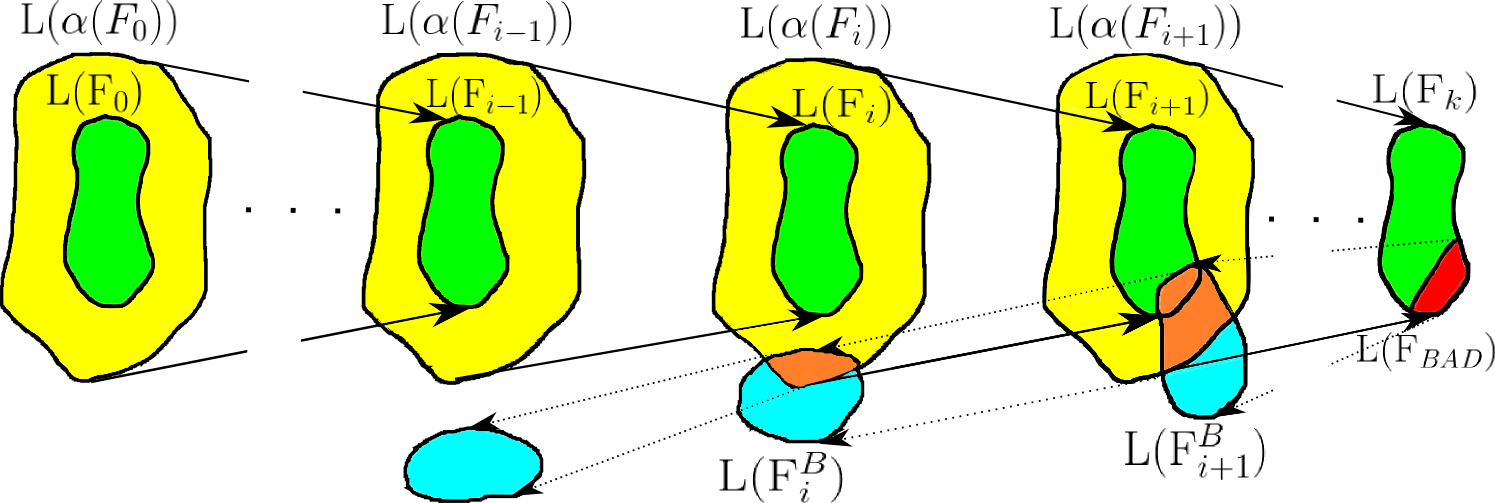
\includegraphics[scale=0.26]{artmc.png}
  \end{itemize}
\end{frame}
%*******************************************************************************
 
%*******************************************************************************
\begin{frame}
\frametitle{Abstraction}

	\begin{itemize}
		\item Overapproximates reachable configurations and accelerates analysis
		\item Collapses states in the same equivalence class of \hlrd{a relation $\sim$}
		\item \hlgr{Height Abstraction}
		\begin{itemize}
			\item Equivalence $\sim_H$ is defined as
				\hlrd{$$q_1 \sim_H q_2 \stackrel{DEF}{\equiv} L^n(q_1) = L^n(q_2)$$}\noindent where
				\hlrd{$L^n(q)$} is the~language of prefixes of trees accepted from $L(q)$ with height up to $n$
			\item \hlbl{Refinement}: By increasing the height
			\item \hlbl{Not informed refinement} $\Rightarrow$ state explosion
		\end{itemize}

		\pause
	    \item \hlgr{Predicate Language Abstraction}
		\begin{itemize}
			\item Given a set of predicate languages $P=\{p_1,\ldots,p_n\}$,
				equivalence~$\sim_P$ is defined as
				\hlrd{$$q_1 \sim_P q_2 \stackrel{DEF}{\equiv} \forall p\in P: L(q_1) \cap p \neq \emptyset \Leftrightarrow L(q_2) \cap p \neq \emptyset$$}
			\item \hlbl{Refinement}: Interpolating languages from counterexamples
			\item \hlbl{Informed refinement} 
		\end{itemize}
	\end{itemize}


\end{frame}

%*******************************************************************************

%*******************************************************************************
\begin{frame}
\frametitle{Backward Run and Abstraction for Forest Automata}
		\begin{itemize}
		\item Counterexample validation via backward run.
		\item \hlgr{Ingredients for backward run}:
		\begin{itemize}
			\item Reversion of \hlbl{abstract transformations}.
			\begin{center}
				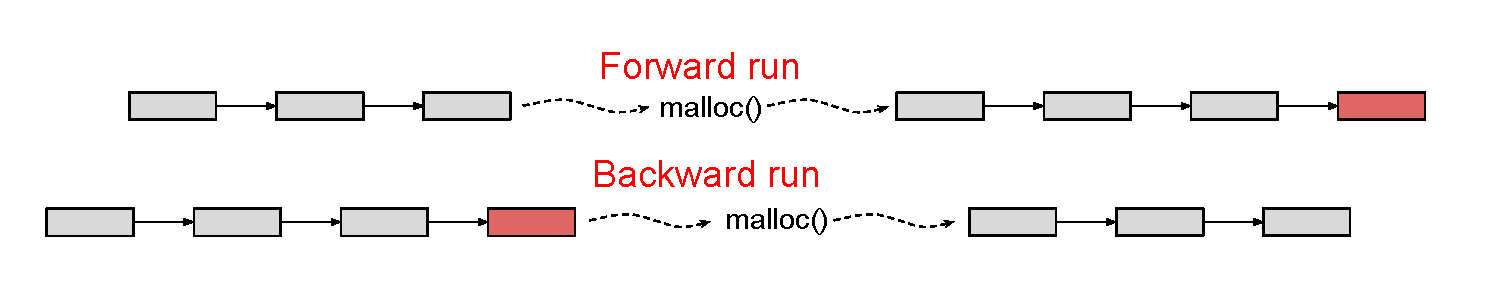
\includegraphics[scale=0.4]{ex/at.pdf}
			\end{center}
			\pause
			\item Reversion of \hlbl{abstraction} $\rightarrow$ \hlgr{intersection} of FA.
			\begin{itemize}
				\item Consider FA $F_1=(TA_1^1,\ldots,TA_n^1)$ and $F_2=(TA_1^2,\ldots,TA_n^2)$,
					intersection is done \hlgr{component-wise} using TA intersection, i.e.,
					$F_1 \cap F_2 = (TA_1^1 \cap TA_1^2,\ldots,TA_n^1 \cap TA_n^2)$.
			\end{itemize}
		\item Precise reversion of folding and unfolding of boxes $\Rightarrow$ \hlrd{compatible form}.
		\end{itemize}
		\pause
		\item \hlgr{Ingredients for predicate language abstraction}:
		\begin{itemize}
			\item Predicate languages represented by TA.
			\item New predicate TAs obtained by intersecting FAs from FW and BW run.
			% \item Needs intersection of TA.
			% \item Obtain a labelling of FA states by predicate automata states.
			% \item Collapses the states with the same labelling.
		\end{itemize}
	\end{itemize}

\end{frame}

%*******************************************************************************

%*******************************************************************************
% \begin{frame}
% \frametitle{Backward run with Hierarchical Forest Automata}
% 	
% 		   	\begin{itemize}
% 				\item To enable component-wise hierarchical FA intersection,
% 					so called \hlbl{compatible form} of FA is needed:
% 				\begin{itemize}
% 					\item They have same number of TA
% 					\item \hlbl{The same subgraphs are folded into the same boxes}
% 				\end{itemize}
% 				\item Compatible form is preserved during backward run
% 			\end{itemize}
% 
% 	\begin{center}
% 		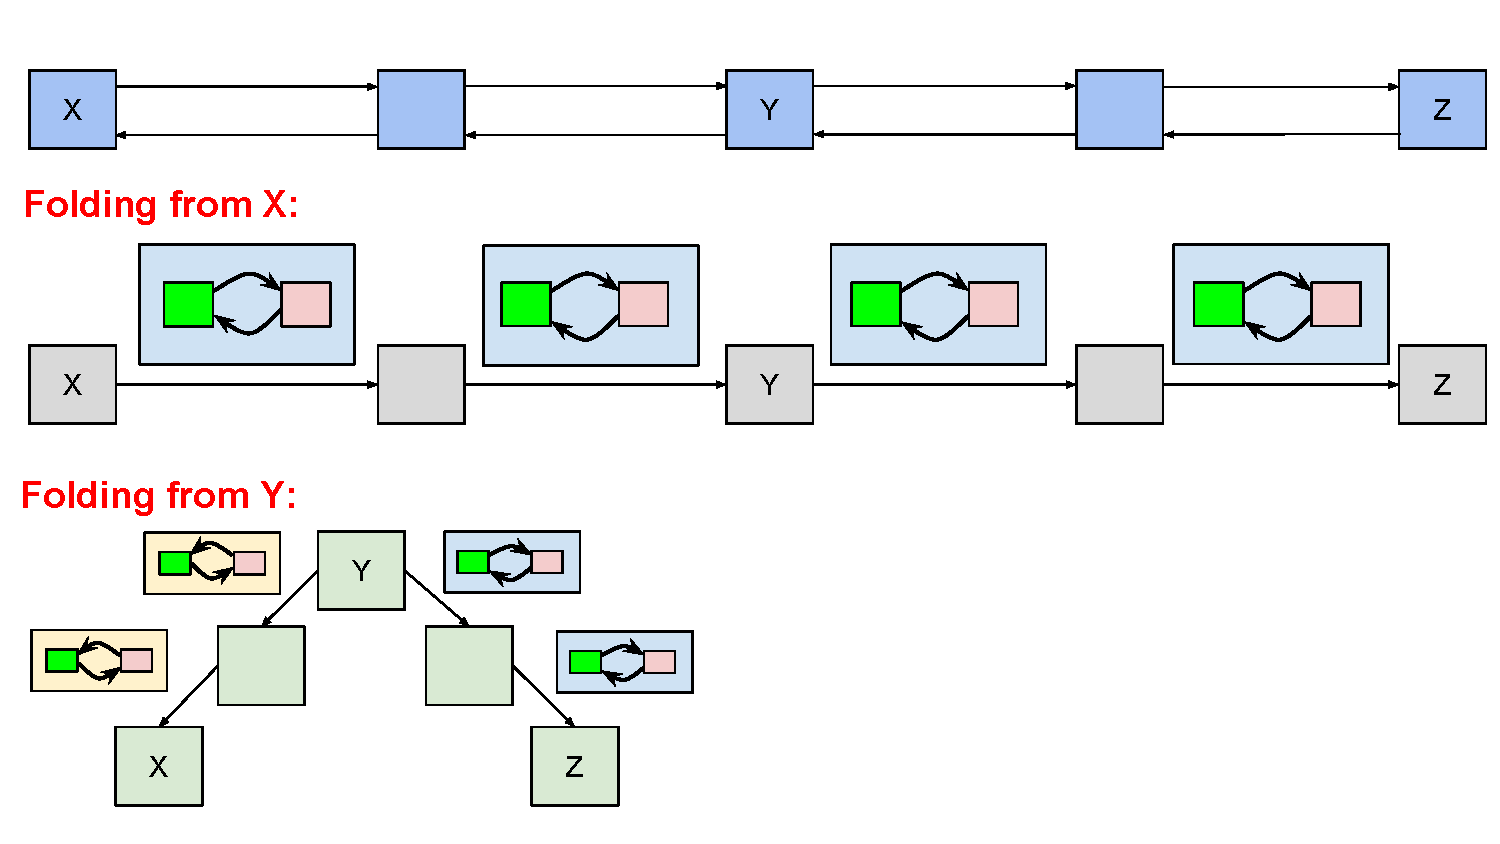
\includegraphics[scale=0.4]{ex/cp.pdf}
% 	\end{center}
% 
% \end{frame}
%*******************************************************************************


%*******************************************************************************
% \begin{frame}
% \frametitle{Intersection with Hierarchical Forest Automata}
% 
%   	\begin{itemize}
% 	\item \hlbl{Intersection of FA} is done:
% 		  	\begin{itemize}
% 				\item Component-wise using TA intersection
% 				\item When TA intersection reaches boxes in the transitions of both automata it calls the whole
% 					procedure for \hlbl{FA intersection recursively on the boxes} and uses its results as a new box
% 			\end{itemize}
% 	\end{itemize}
% 	\begin{center}
% 		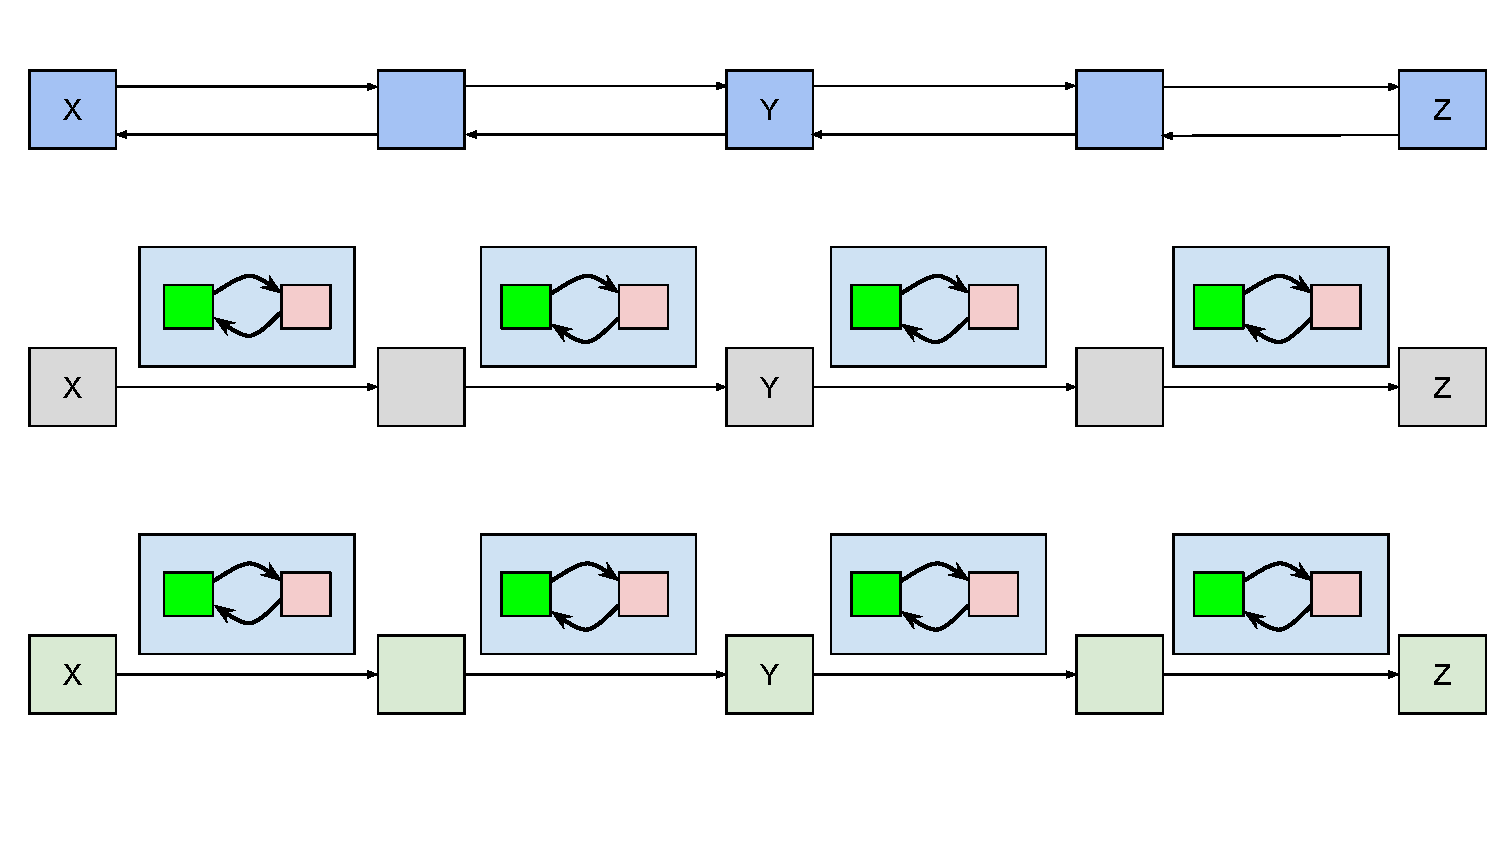
\includegraphics[scale=0.4]{ex/is.pdf}
% 	\end{center}
% 
% \end{frame}
%*******************************************************************************

%*******************************************************************************
\begin{frame}
\frametitle{Experimental Evaluation}
    \begin{itemize}
        \item Shape analysis based on Forest automata implemented in the \hlrd{Forester} tool
    \end{itemize}
	\begin{center}
	\begin{adjustbox}{max height=\textheight, max width=\textwidth}
	%\tiny
	%\caption{Results of experiments.}
	\begin{tabular}{| l | l | r | r | r | r || l | l | r | r | r | r | r |}
        \hline
		Program & Status & LoC & Time [s] & Refnm& Preds & Program & Status & LoC & Time [s] & Refnm & Preds \\
        \hline
        \hline
		SLL (delete) & \cellcolor{\scol{}} \safe & $33$ & $0.02$ &  $0$ & $0$ & DLL (rev) & \cellcolor{\scol{}} \safe & $39$ &  $0.70$ & $0$  & $0$ \\
        \hline
		SLL (bubblesort) & \cellcolor{\scol{}} \safe & $42$ & $0.02$ &  $0$ & $0$ & CDLL & \cellcolor{\scol{}} \safe & $32$ &  $0.02$  & $0$  & $0$ \\
        \hline
		SLL (insertsort) & \cellcolor{\scol{}} \safe & $36$ & $0.04$ & $0$ & $0$ & DLL (insertsort) & \cellcolor{\scol{}} \safe & $42$ &  $0.56$  & $0$  & $0$ \\
        \hline
		SLLOfCSLL & \cellcolor{\scol{}} \safe & $47$ & $0.02$ & $0$ & $0$ & DLLOfCDLL & \cellcolor{\scol{}} \safe & $54$ &  $1.76$  & $0$  & $0$ \\
        \hline
		\rowcolor{\hcol{}}
		\textbf{SLL01}    & \cellcolor{\scol{}} \safe & $70$ & $1.20$   &  $1$ & $1$ & \textbf{DLL01} & \cellcolor{\scol{}} \safe & $73$ &  $0.65$  & $2$  & $2$ \\
        \hline
		\rowcolor{\hcol{}}
		\textbf{CircularSLL} & \cellcolor{\scol{}} \safe & $49$ & $3.57$   &  $3$  & $3$ & \textbf{CircularDLL} & \cellcolor{\scol{}} \safe  & $52$ &  $37.22$ & $18$ & $24$ \\
        \hline
		\rowcolor{\hcol{}}
		\textbf{OptPtrSLL}   & \cellcolor{\scol{}} \safe & $59$ & $1.90$ & $3$ & $3$ & \textbf{OptPtrDLL} &\cellcolor{\scol{}} \safe & $62$ &  $1.87$  & $5$ & $5$ \\
        \hline
		\rowcolor{\hcol{}}
		\textbf{QueueSLL}    & \cellcolor{\scol{}} \safe & $71$ & $11.32$  &  $10$ & $10$ & \textbf{QueueDLL} &  \cellcolor{\scol{}}  \safe  & $74$ &  $44.68$ & $14$ & $14$ \\
		\rowcolor{\hcol{}}
        \hline
		\textbf{GBSLL}       & \cellcolor{\scol{}} \safe & $64$ & $0.84$   &  $3$ & $3$ & \textbf{GBDLL} &  \cellcolor{\scol{}}  \safe & $71$ &  $1.89$  & $4$ & $4$ \\
        \hline
		\rowcolor{\hcol{}}
		\textbf{GBSLLSent}   & \cellcolor{\scol{}} \safe  & $68$ & $0.85$   &  $3$ & $3$ & \textbf{GBDLLSent} & \cellcolor{\scol{}} \safe & $75$ &  $2.19$  & $4$ & $4$ \\
        \hline
		\rowcolor{\hcol{}}
		\textbf{RGSLL}       & \cellcolor{\scol{}} \safe & $72$ & $14.41$  &  $22$  & $38$ & \textbf{RGDLL} & \cellcolor{\scol{}} \safe & $76$ &  $78.76$ & $26$ & $26$ \\
        \hline
		\rowcolor{\hcol{}}
		\textbf{WBSLL}       & \cellcolor{\scol{}} \safe & $62$ & $0.84$   &  $5$  & $5$ & \textbf{WBDLL} & \cellcolor{\scol{}} \safe & $71$ &  $1.37$  & $7$ & $7$ \\
        \hline
		\rowcolor{\hcol{}}
		\textbf{SortedSLL}   & \cellcolor{\scol{}} \safe & $76$ & $227.12$ &  $15$ & $15$ & \textbf{SortedDLL} & \cellcolor{\scol{}} \safe & $82$ &  $36.67$ & $11$ & $11$ \\
        \hline
		\rowcolor{\hcol{}}
		\textbf{EndSLL}      & \cellcolor{\scol{}} \safe  & $45$ & $0.07$   &  $2$  & $2$ & \textbf{EndDLL} & \cellcolor{\scol{}} \safe & $49$ &  $0.10$  & $3$ & $3$ \\
        \hline
		\rowcolor{\hcol{}}
		\textbf{TreeRB} & \cellcolor{\ucol{}}\unsafe & $130$ &  $0.08$  & $0$  & $0$ & \textbf{TreeWB} & \cellcolor{\ucol{}}\unsafe & $125$ &  $0.05$  & $0$ & $0$ \\
        \hline
		TreeCnstr & \cellcolor{\scol{}} \safe & $52$ & $0.31$  & $0$  & $0$ & \cellcolor{\hcol{}}\textbf{TreeCnstr} & \cellcolor{\ucol{}}\unsafe & \cellcolor{\hcol{}} $52$ & \cellcolor{\hcol{}} $0.03$  & \cellcolor{\hcol{}} $0$ & \cellcolor{\hcol{}} $0$ \\
        \hline
		TreeOfCSLL & \cellcolor{\scol{}} \safe & $109$ &  $0.57$  & $0$  & $0$ & \cellcolor{\hcol{}}\textbf{TreeOfCSLL}  & \cellcolor{\ucol{}}\unsafe & \cellcolor{\hcol{}} $109$ & \cellcolor{\hcol{}} $0.56$  & \cellcolor{\hcol{}} $1$ & \cellcolor{\hcol{}} $3$ \\
        \hline
		TreeStack & \cellcolor{\scol{}} \safe & $58$ &  $0.20$  & $0$  & $0$ & \cellcolor{\hcol{}}\textbf{TreeStack} & \cellcolor{\ucol{}}\unsafe & \cellcolor{\hcol{}} $58$ & \cellcolor{\hcol{}} $0.01$  & \cellcolor{\hcol{}} $0$ & \cellcolor{\hcol{}} $0$ \\
        \hline
		TreeDSW   & \cellcolor{\scol{}} \safe & $72$ & $1.87$  & $0$  & $0$ & \cellcolor{\hcol{}}\textbf{TreeDSW} & \cellcolor{\ucol{}}\unsafe & \cellcolor{\hcol{}} $72$ & \cellcolor{\hcol{}} $0.02$  & \cellcolor{\hcol{}} $0$ &  \cellcolor{\hcol{}} $0$ \\
		\hline
		TreeRootPtr & \cellcolor{\scol{}} \safe & $62$ &  $1.43$  & $0$  &  $0$ & \cellcolor{\hcol{}}\textbf{TreeRootPtr} & \cellcolor{\ucol{}}\unsafe & \cellcolor{\hcol{}} $62$ & \cellcolor{\hcol{}} $0.17$  & \cellcolor{\hcol{}} $2$ & \cellcolor{\hcol{}} $6$\\
        \hline
		SkipList    & \cellcolor{\scol{}} \safe & $84$ & $3.36$  & $0$  & $0$ & \cellcolor{\hcol{}}\textbf{SkipList} & \cellcolor{\ucol{}}\unsafe & $\cellcolor{\hcol{}} 84$ & \cellcolor{\hcol{}} $0.08$  & \cellcolor{\hcol{}} $1$  & \cellcolor{\hcol{}} $1$ \\
        \hline
		% SkipList-3nd    & $97$ & $0.17$  & $1$  & N & x & $1$ & & & & & & & \\
        % \hline
	\end{tabular}
	\label{tab:times}
	\end{adjustbox}	
  % \vspace{-4mm}
  % \vspace{-8mm}
%\end{table}
	\end{center}

\end{frame}
%*******************************************************************************

%*******************************************************************************
\frame{\frametitle{Forester in SV-COMP}
	\begin{itemize}
	  \item<1-> Forester competed in SV-COMP in years 2015-2018 in the \hlbl{categories related to memory safety} (\emph{MemSafety, HeapReach}).
          \item<2-> \hlrd{2015}
	  \begin{itemize}
            \item Using the VATA library for tree automata as backend.
            \item Counterxample witness generation. 
	  \end{itemize}
          \item<3-> \hlrd{2016}
	  \begin{itemize}
            \item Added support to run Forester using Benchexec.
            \item Counterexample analysis and abstraction refinement for basic forest automata.
	  \end{itemize}
          \item<4-> \hlrd{2017}
	  \begin{itemize}
            \item Generating correctness witness (forest automaton representing shape invariants of program).
            \item Counterexample analysis and abstraction refinement for hierarchical forest automata.
	  \end{itemize}
          \item<4-> Forester has never won any medal, but was able to verify difficult data structures (skip-lists or various trees) which were not solved by any other tool.
	\end{itemize}
}
%*******************************************************************************

%*******************************************************************************
\frame{\frametitle{ }
	\begin{center}
    	\large \hlgr{Towards Efficient Shape Analysis with Tree Automata}

		\vspace{1cm}

		\small{Hol{\'{\i}}k, L., \hlbl{Hru\v{s}ka, M.} NETYS'21.}
	\end{center}
}
%*******************************************************************************

%*******************************************************************************
\frame{\frametitle{Towards Efficient Shape Analysis with Tree Automata (TA)}
	% \begin{itemize}
	%   \item Forest Automata have their limits:
	%   \begin{itemize}
	%     \item Can't represent data structures such as grid (unbounded number of cut-points).
        %     \item Are not closed under union (which complicates their manipulation during verification procedure, e.g., a fixpoint computation).
	% \end{itemize}
        % \pause
	\begin{itemize}
        \item We proposed new automata able to represent \hlbl{graphs with bounded tree-width}.
        \item They are based on tree automata but we work with single TA instead of tuple of TA (like in FA).  
        \item We sketched \hlbl{efficient algorithm for entailment} for these automata.
        \end{itemize}
}
%*******************************************************************************


%*******************************************************************************
\frame{\frametitle{Tree Decomposition with Variables}
	\begin{itemize}
          \item How to represent a graph with bounded tree-width by a tree automaton? By tree decompositions with \hlbl{variables}.
	\end{itemize}
        \begin{center}
          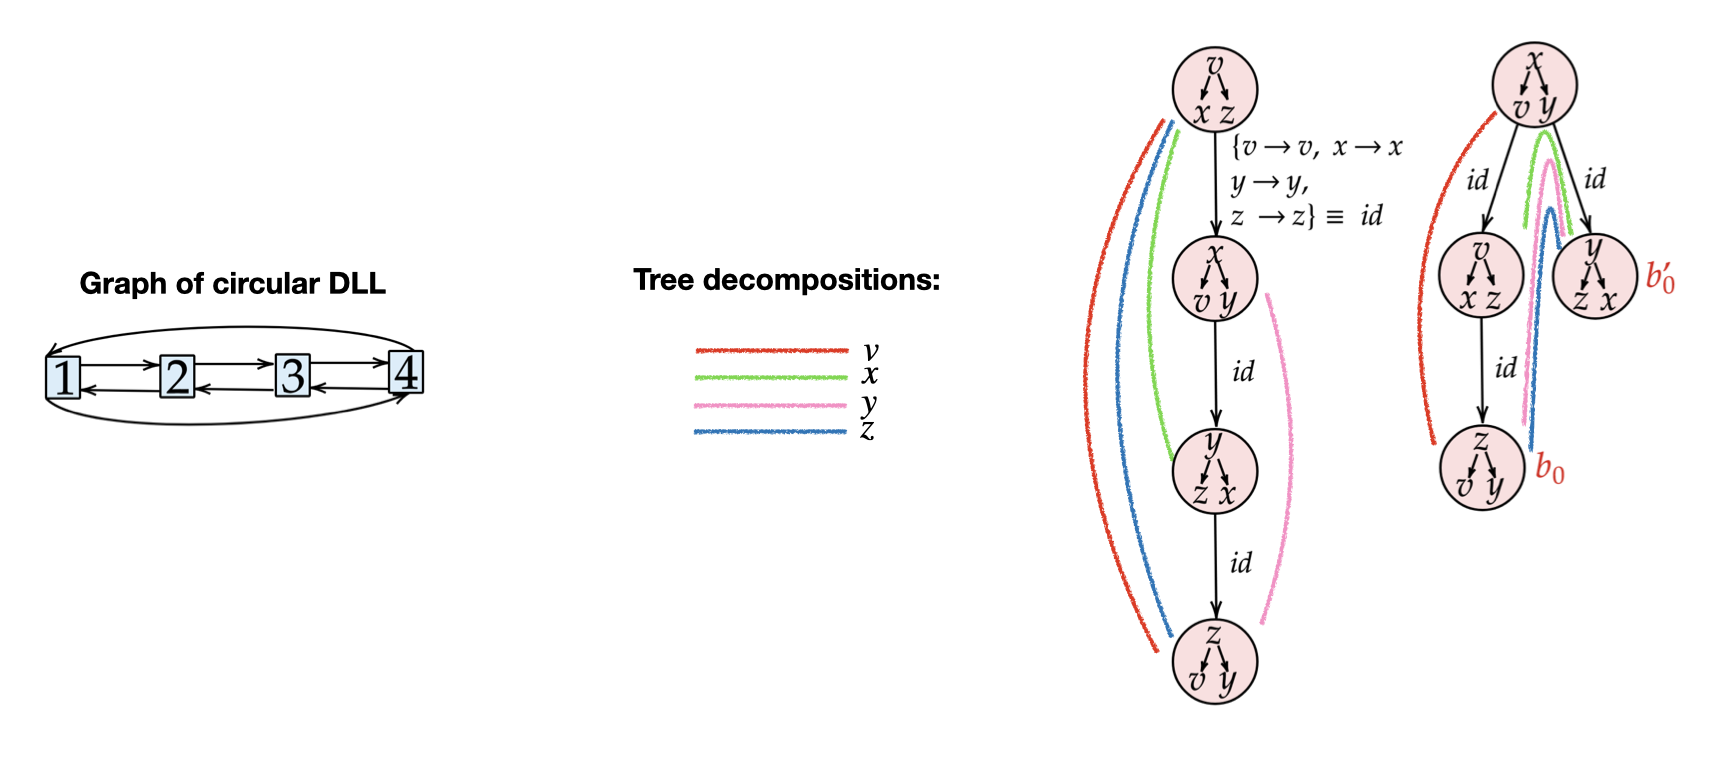
\includegraphics[scale=0.18]{figs/netys/tree_decomp.png}
 	\end{center}
        \vspace{-1em}
}
%*******************************************************************************

%*******************************************************************************
\frame{\frametitle{Towards Entailment}
	  \begin{itemize}
            \item<1-> A graph may have more decompositions and we want a TA to represent all of them (\hlbl{shape invariant}).
            \item<2-> We can create TA representing all tree decompositions that is of a \hlbl{polynomial size assuming a fixed tree-width} of the original automaton.
            \item<3-> Since automata inclusion is EXPTIME-complete, we have entailment which is \hlbl{singly exponential} (assuming a fixed maximum tree width).
            % \item<2-> We need two operations, \hlbl{rotation} and \hlbl{reconnection}, over TA to be able to do that.
            % \item<3-> \hlbl{Phase} is a set of all operations that could be performed at once (they don’t interfere with each other).
            % \vspace{1em}
            % \item<4-> The implementation of a \hlbl{tree automata phase at most doubles the number of variables} and leads to \hlbl{an automaton that is of a polynomial size assuming a fixed tree-width} of the original automaton.
            % \vspace{1em}
            % \item<5-> Since automata inclusion is EXPTIME-complete, we have entailment which is \hlbl{singly exponential} (assuming a fixed maximum tree width).
	  \end{itemize}
}
%*******************************************************************************

%*******************************************************************************
% \frame{\frametitle{Towards Efficient Shape Analysis with Tree Automata}
% 	\begin{itemize}
%           \item A \emph{tree decomposition} of a labeled graph $g$ over a finite set of variables $\vars$ and alphabet $\Sigma$ is a~tree $\dec=(\bubbles,\edgs)$.
%             Nodes $\bubbles$ of $t$ are $\Sigma$-labeled graphs called \emph{bags}. Nodes of a bag are variables from $\vars$.
%             Edges of $\dec$ are labelled by partial mappings $\rho:\vars\rightarrow\vars$ called \emph{parameter assignments}.
% 	\end{itemize}
%  	\begin{center}
%        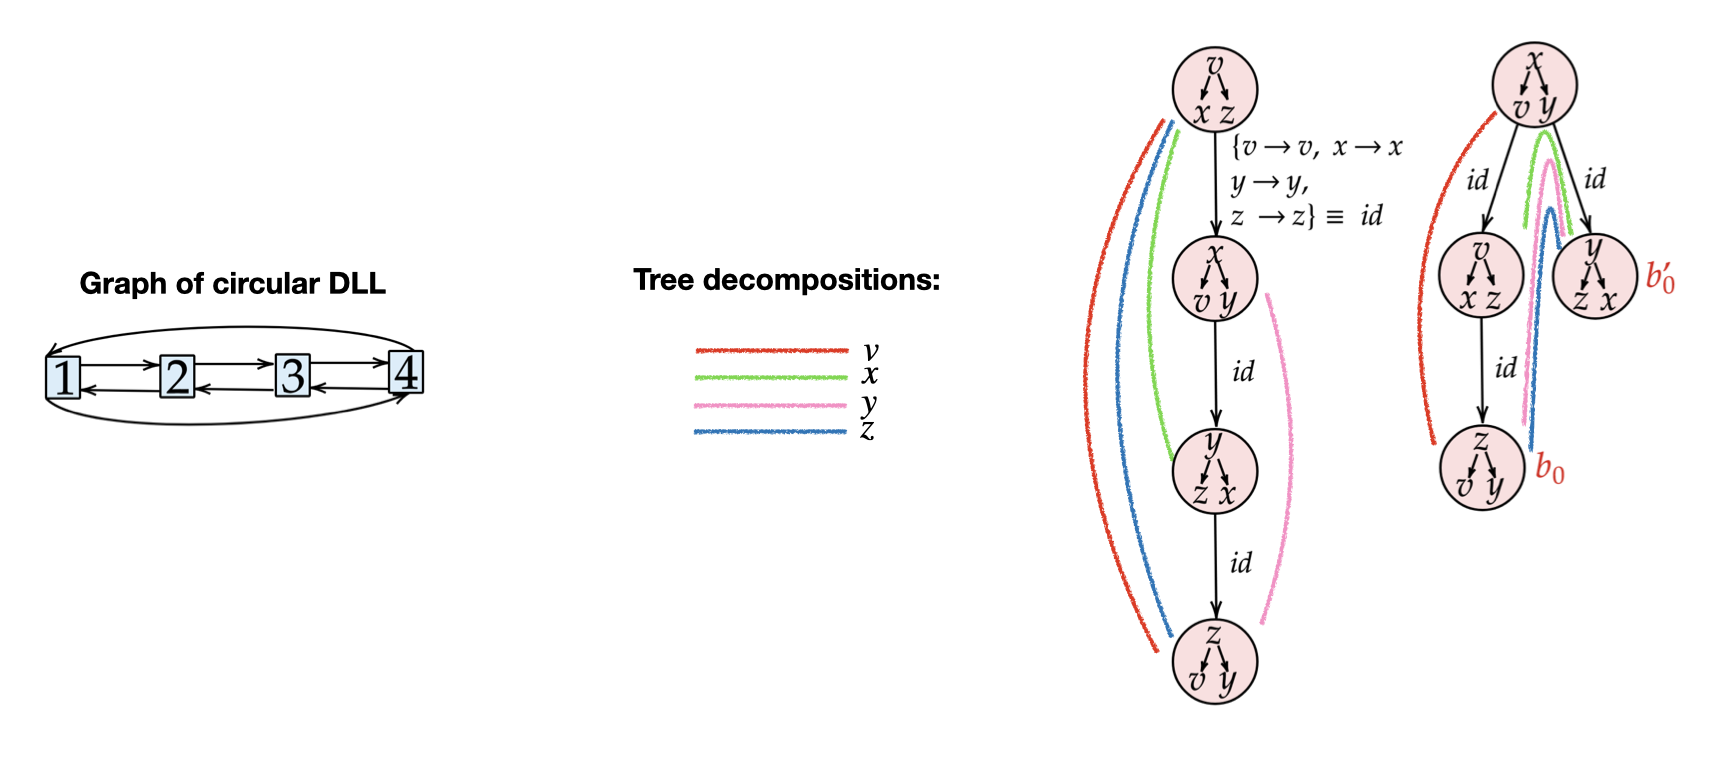
\includegraphics[scale=0.2]{figs/netys/tree_decomp.png}
%  	\end{center}
% }
% %*******************************************************************************
% 
% %*******************************************************************************
% \frame{\frametitle{Automata over Graphs with Bounded Tree-width}
% 	\begin{itemize}
%           \item Reconnection - moving the bag $b_0$ under the bag $b_0'$.
% 	\end{itemize}
%  	\begin{center}
%  	\begin{figure*}
%  		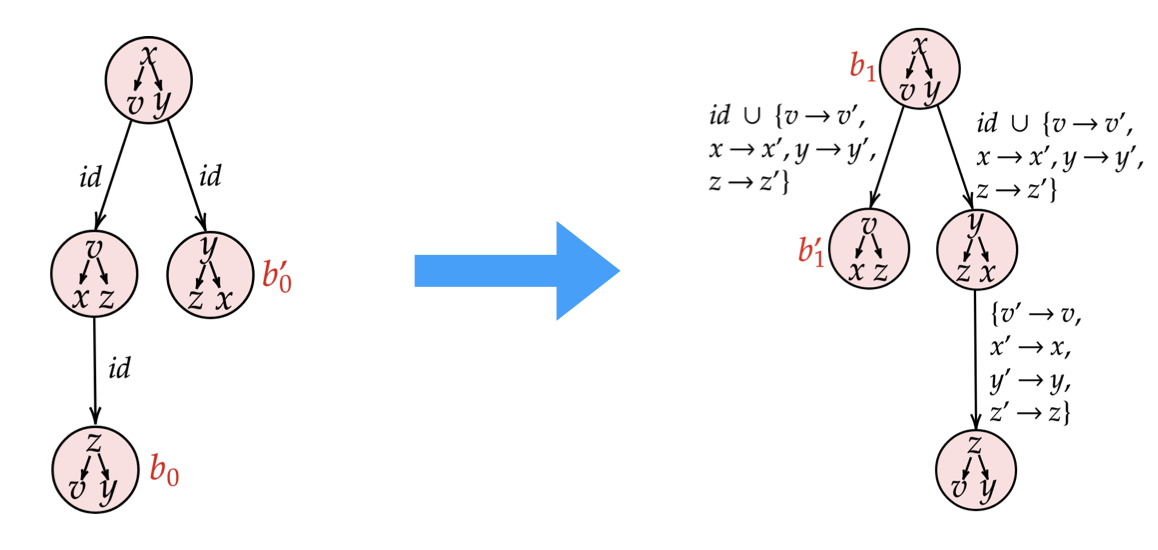
\includegraphics[scale=0.3]{figs/netys/decomp1.png}
%  	\end{figure*}
%  	\end{center}
% }
% %*******************************************************************************
% 
% %*******************************************************************************
% \frame{\frametitle{Automata over Graphs with Bounded Tree-width}
% 	\begin{itemize}
%           \item Rotation - changing orientation of the edge between $b_1$ and $b_1'$
% 	\end{itemize}
%  	\begin{center}
%  	\begin{figure*}
%  		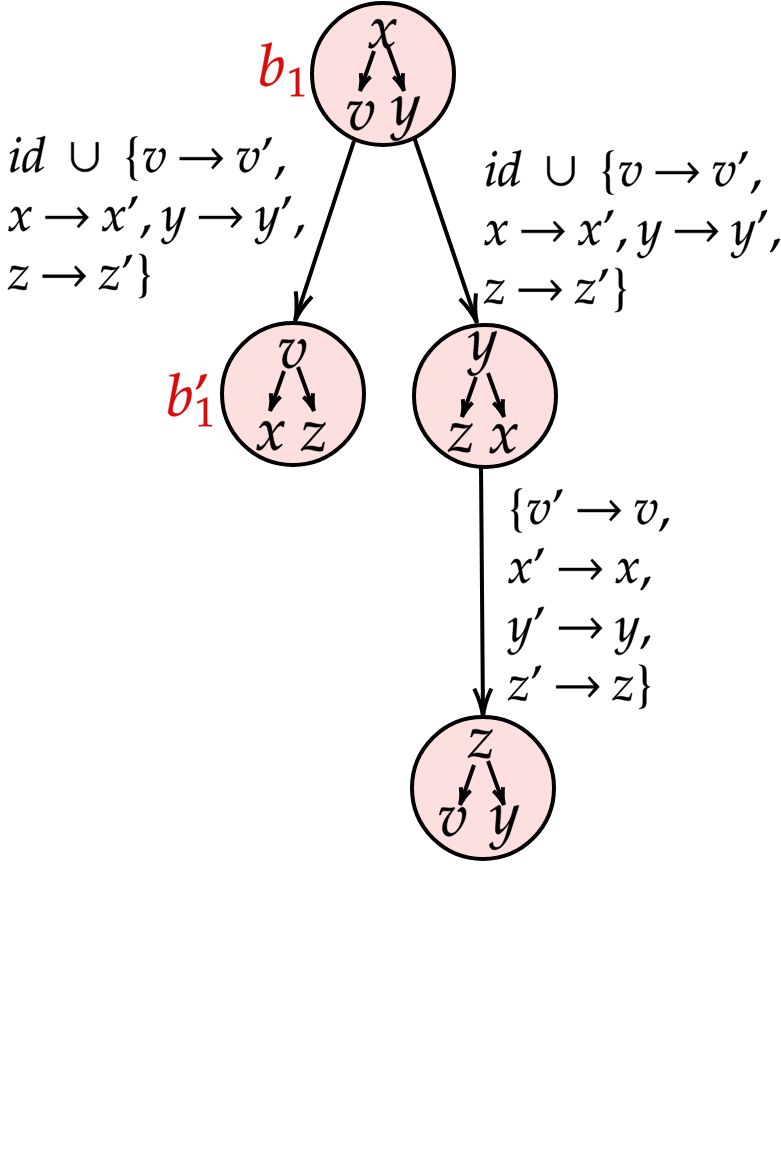
\includegraphics[scale=0.25]{figs/netys/decomp2.png}
%  	\end{figure*}
%  	\end{center}
% }
%*******************************************************************************


%*******************************************************************************
%\frame{\frametitle{Towards entailment}
%	  \begin{itemize}
%            \item<1-> \hlbl{Phase} is a set of all operations that could be performed at once (they don’t interfere with each other).
%            \item<2-> One phase at most doubles the number of variables.
%            \item<3-> \hlbl{An equivalent decomposition $t$ can be obtained from $t'$} in a number of phases that depends only on \hlbl{$max(tw(t),tw(t'))$} where $tw$ is a tree width of decomposition.
%            \vspace{1em}
%            \item<4-> Tree decompositions can be represented by language of \hlbl{tree automaton}.
%            \item<5-> Rotation and reconnection can be performed also on tree automata (e.g., using tree transducer).
%            \item<6-> The implementation of a \hlbl{tree automata phase at most doubles the number of variables} and leads to \hlbl{an automaton that is of a polynomial size assuming a fixed tree-width} of the original automaton.
%            \vspace{1em}
%            \item<7-> Since automata inclusion is EXPTIME-complete, we have entailment which is \hlbl{singly exponential} (assuming a fixed maximum tree width).
%	  \end{itemize}
%}
%*******************************************************************************

%*******************************************************************************
\frame{\frametitle{}
	\begin{center}
    	\large \hlgr{Shape Analysis based on SMT Solving in 2LS Framework}

		\vspace{1cm}

		\small{Mal{\'{\i}}k, V., \hlbl{Hru\v{s}ka, M.}, Schrammel P., Vojnar T. FMCAD'18.}
	\end{center}
}
%*******************************************************************************

%*******************************************************************************
\frame{\frametitle{Shape Analysis based on SMT Solving in 2LS Framework}
	\begin{itemize}
          \item Shape analysis using \hlbl{SMT solving} to compute the points-to relation between pointers and (abstract) memory addresses.
          \item Domain designed for \hlbl{representation of linked-lists}.
          \item Therefore more straightforward than the automata-based approaches, but lacks thier generality.
          \pause
          \item Implemented within \hlbl{the 2LS framework} for program analysis.
	  \begin{itemize}
            \item Combination with other domains in the framework, e.g., the numerical domain.
	  \end{itemize}
	\end{itemize}
}
%*******************************************************************************

%*******************************************************************************
\frame{\frametitle{Shape Analysis based on SMT Solving in 2LS Framework}
        \begin{itemize}
          \item Verification procedure takes:
	  \begin{itemize}
            \item A \hlbl{first order formula over combination of SMT theories} that represents the program in SSA form (i.e., transition relation).
            \item A \hlbl{set of invariants based on predefined templates} (proposed for various domains).
            \item \hlbl{The property of interest} (e.g., memory safety properties).
	  \end{itemize}
          \pause
           \item And verifies that there is no reachable invariants violate the properties of interest.
          \pause
          \item The template for shape analysis is: $\templ^S \equiv \bigwedge_{\ssaplb{i} \in \ptrlb} = \templ^S_{\ssaplb{i}}(d_{\ssaplb{i}})$,
	    \begin{itemize}
              \item where \hlbl{$\templ^S_{\ssaplb{i}}(d_{\ssaplb{i}}) \equiv (\bigvee_{a \in d_{\ssaplb{i}}} \ssaplb{i} = a)$}.
              \item Basically, it describes the points-to relation between a pointer ($\ssaplb{i}$) and addresses $a$ that the pointer may point to.
	    \end{itemize}
	\end{itemize}
}
%*******************************************************************************

%*******************************************************************************
% \frame{\frametitle{Shape Analysis based on SMT Solving in 2LS Framework}
% 	\begin{itemize}
%            \item Technically, unsatisfiability of this formula:
% 	  \begin{itemize}
%             \item $\exists \vx, \vxp .\; \neg (\fminit(\vx) \Longrightarrow \templ(\vx, \vd)) \; \vee \neg (\templ(\vx, \vd) \wedge \fmtrans(\vx,\vxp) \Longrightarrow \templ(\vxp, \vd))$
%            \item  where $\fminit(\vx)$ is an initial state of variables, $\templ$ is a set of invariants based on templates, $\fmtrans$ formula representing program
% 	  \end{itemize}
%           \pause
%           	\end{itemize}
% }
%*******************************************************************************

%*******************************************************************************
\frame[shrink=5]{\frametitle{Experimental Evaluation}
%%%%%%%%%%%%%%%%%%%%%%%%%%%%%%%%%%%%%%%%%%%%%%%%%%%%%%%%%%%%%%%%%%%%%5
\newcolumntype{g}{>{\columncolor{LightCyan}}r}
\begin{table}[bt]
\small
\captionsetup{font=small}
\caption{Comparison of 2LS with other tools on examples that need reasoning about unbounded data structures and their stored data.}
\vspace*{-1mm}
\label{tab:others}
\centering
\scriptsize
\bgroup
\def\arraystretch{1.2}
\begin{tabular}{|l| g | r | r | r | r | r |}
\hline
& \textbf{2LS}  & \textbf{CPA-Seq } & \textbf{PredatorHP} & \textbf{\forester}  & \textbf{Symbiotic} & \textbf{UAutomizer}  \\\hline
Calendar          & 2.88   & timeout & false   & unknown  & timeout  & timeout  \\\hline
Cart              & 23.70  & timeout & false   & unknown  & timeout  & timeout  \\\hline
Hash Function     & 3.65   & 8.51    & unknown & unknown  & unknown  & timeout  \\\hline
MinMax            & 5.14   & timeout & false   & unknown  & timeout  & timeout  \\\hline
Packet Filter     & 431.00 & timeout & timeout & unknown  & unknown  & timeout  \\\hline
Process Queue     & 6.62   & 7.68    & timeout & unknown  & timeout  & timeout  \\\hline
Quick Sort        & 18.20  & 3.50    & timeout & unknown  & unknown  & 5.75     \\\hline
Running Example   & 1.24   & timeout & timeout & unknown  & timeout  & unknown  \\\hline
SM1               & 0.53   & timeout & 0.31    & false    & timeout  & timeout  \\\hline
SM2               & 0.55   & 5.41    & false   & false    & timeout  & 14.50    \\\hline
\end{tabular}
\egroup
\vspace{-1.5em}
\end{table}
%%%%%%%%%%%%%%%%%%%%%%%%%%%%%%%%%%%%%%%%%%%%%%%%%%%%%%%%%%%%%%%%%%%%%5
}
%*******************************************************************************

%*******************************************************************************
\frame{\frametitle{Automated Software Testing (with Automata)}
	\begin{center}
    	\large \hlgr{Generating Scenarios for Digital Twins of Distributed Manufacturing Execution Systems.}

		\vspace{1cm}

		\small{Fiedor, T., \hlbl{Hru\v{s}ka, M.}, Smr\v{c}ka, A. EUROCAST'22.}
	\end{center}
}
%*******************************************************************************

%*******************************************************************************
\frame{\frametitle{Introduction}
  \begin{itemize}
    \item \hlrd{Manufacturing Execution System (MES)}
    \begin{itemize}
      \item Software managing production in factory.
      \item Communicates with information system, machines, and other components.
      \item Difficult to test:
      \begin{itemize}
         \item Distributed nature of manufacturing, different communication protocols, different formats of messages.
     %   \item Distributed nature of manufacturing, different communication protocols, different formats structured data.
       % \item Communication with Enterprise Resource Planning (ERP) systems such as SAP, e.g., checking quantity of material in stocks.
       % \item Scheduling production over the machines.
       % \item Controlling and communicating with machines during production.
       % \item Processes inputs by human workers operating machines.
      \end{itemize}
  \end{itemize}
      \pause
    \item \hlrd{Digital twin}
    \begin{itemize}
      \item Generally, digital copy of a cyber-physical system\,---\,simulation of reality on computer, often with graphical interface.
      \item Not everything needs to be simulated, some software may be used in digital twin natively.
    \end{itemize}
     % \item \hlbl{Testing of MES is difficult because}:
     %  \begin{itemize}
     %   \item Distributed nature of manufacturing, different communication protocols, different formats structured data.
     %   \item Nondeterministic factors\,---\,human workers and their interactions with machines, physical aspects of machines.
     %  \end{itemize}
      \pause
    \item Project solved with the Unis company (\hlbl{MES Pharis}) and Masaryk University (\hlbl{Cryton} for orchestrating digital twin)
    \end{itemize}
}
%*******************************************************************************

% %*******************************************************************************
% \frame{\frametitle{Introduction\,---\,Digital Twin}
%   \begin{itemize}
%     \item \hlrd{Digital twin}
%     \begin{itemize}
%       \item Generally, digital copy of a cyber-physical system\,---\,simulation of reality on computer, often with graphical interface.
%       \item Not everything needs to be simulated, some software may be used in digital twin natively.
%       \pause
%     \end{itemize}
%     \item \hlrd{Our use case}
%     \begin{itemize}
%       \item Particularly, machines, ERP, or human workers are simulated.
%       \item MES is executed natively.
%       \item Can be orchestrated (deployed and controlled) by an input scenario (step by step).
%     \end{itemize}
%   \end{itemize}
% }
% %*******************************************************************************
% 
% %*******************************************************************************
% \frame{\frametitle{Context of the Project}
%   \begin{itemize}
% 	  \item In collaboration with \hlbl{Masaryk University} and \hlbl{UNIS, a.s.} company
%           \item The goal of project was to develop digital twin of systems controlled by MES \hlbl{Pharis }developed by UNIS company
%           \item The presented talk is about learning models of communication and generating scenarios for orchestrating digital twin
%           \item Digital twin was implemented by Masaryk University (\hlbl{the Cryton tool})
%   \end{itemize}
% }
% %*******************************************************************************

%*******************************************************************************
% \frame{\frametitle{Real System}
%     \begin{center}
%      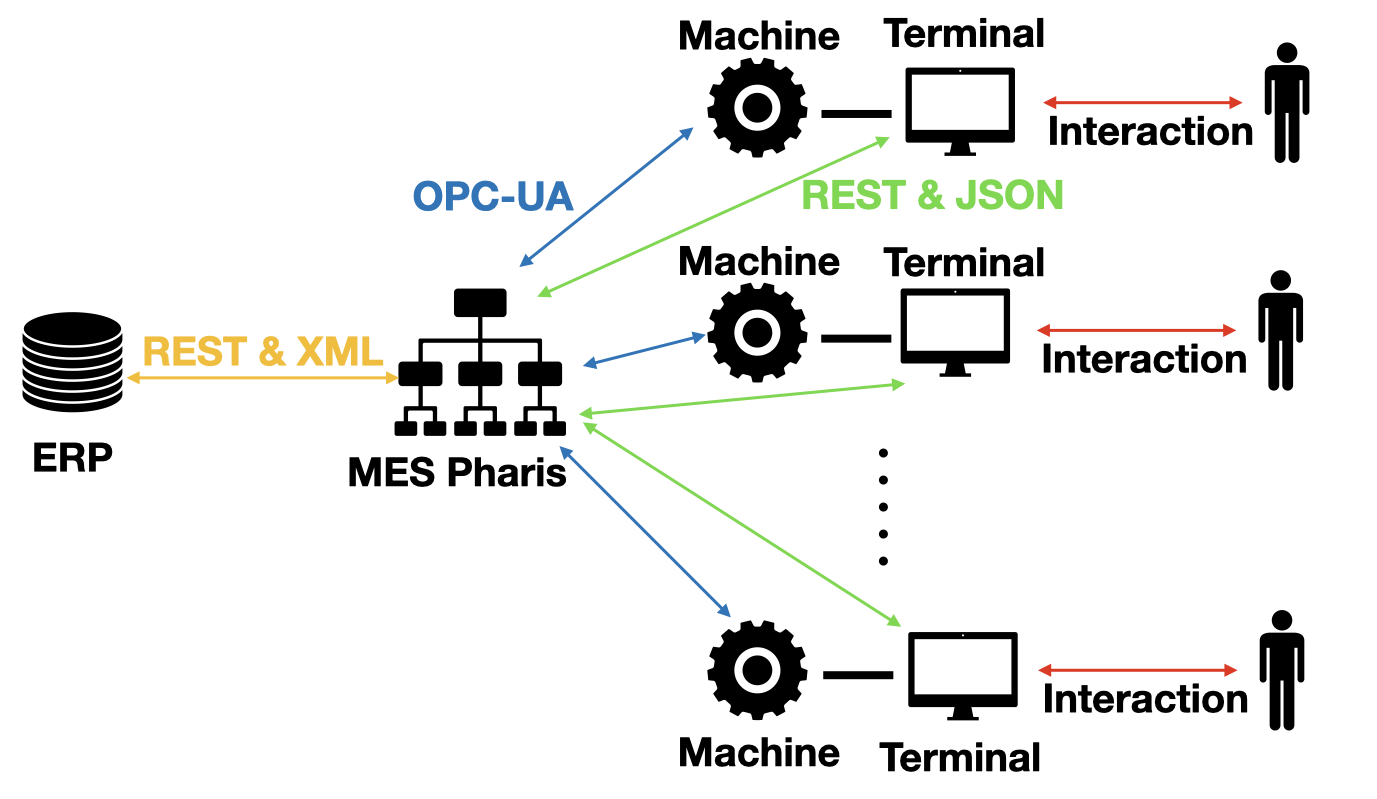
\includegraphics[scale=0.23]{figs/eurocast/real-system.png}
%     \end{center}
% }
%*******************************************************************************

%*******************************************************************************
\frame{\frametitle{Our Solution}
    \begin{center}
      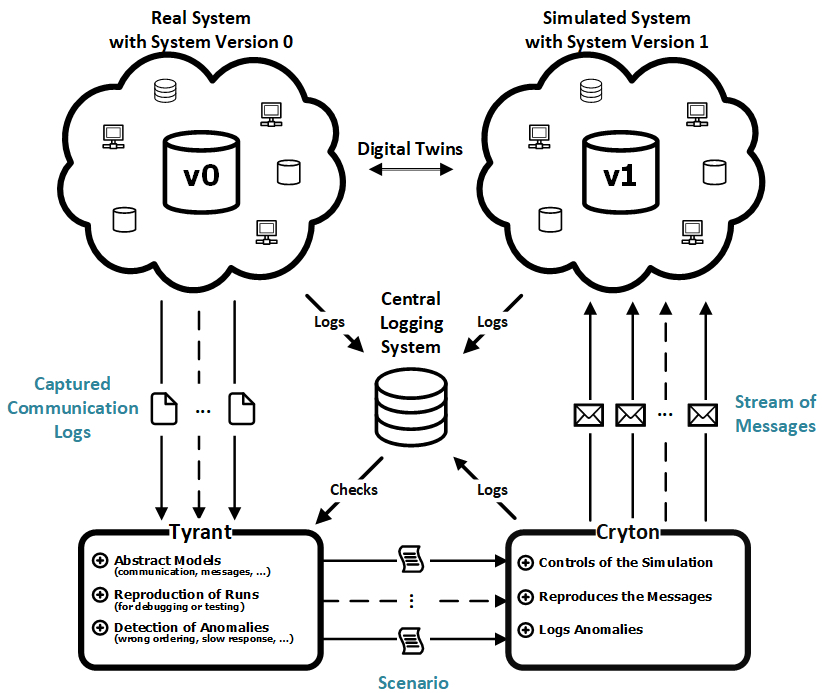
\includegraphics[scale=0.3]{figs/eurocast/tunis-diagram.jpg}
    \end{center}
}
%*******************************************************************************

%*******************************************************************************
\frame{\frametitle{Our Solution}
\begin{itemize}
  \item Representing messages in different formats (XML, or JSON) using \hlbl{Trie} structure (prefix tree)
    \pause
  \item Representing communication using \hlbl{event calendar}.
  \begin{itemize}
    \item Direct generation of scenario for digital twin.
    \item Transformation to finite automaton\,---\,application of abstraction to overapproximate langauge.
    \item New strings in overapproximated langauge $\Rightarrow$ new series of events $\Rightarrow$ new scenario $\Rightarrow$ \hlbl{new test case}.
  \end{itemize}
  \pause
  \item Implemented in the \hlbl{Tyrant} tool.
  \begin{itemize}
    \item Generated valid scenarios for testing MES Pharis. 
    \item More engineering work needed to be deployed in production. 
  \end{itemize}
\end{itemize}
}
%*******************************************************************************

%*******************************************************************************
% \frame{\frametitle{Our Solution}
% \begin{itemize}
%   \item Representing messages with structured data
%   \begin{itemize}
%     \item Different formats of messages\,---\,JSON and XML
%     \item Generic representation and unified manipulation using \hlbl{Trie} structure (prefix tree)
%     \item We classify messages \hlbl{based on structural similarity to different classes} and create an abstract representation of each class.
%     \item Can automatically generate new messages from abstract representation.
%   \end{itemize}
%     \pause
%   \item Representing model of communication:
%   \begin{itemize}
%     \item Representing communication in system using \hlbl{event calendar}.
%     \item There is created an event in calendar for each message (containing sender, receiver, type of message, etc.).
%     \item Later serialized to a YAML scenario used for orchestrating digital twin.
%   \end{itemize}
%     \pause
%   \item Implemented in the \hlbl{Tyrant} tool.
% \end{itemize}
% }
% %*******************************************************************************
% 
% %*******************************************************************************
% \frame{\frametitle{Automata Abstraction to Generate New Tests Cases}
% \begin{itemize}
%   \item Transform event calendar to \hlbl{finite automaton}\,---\,set of events is used as alphabet of automaton.
%   \item Use \hlbl{length abstraction of automaton} to overapproximates language of automaton (merges states of automaton with the same prefix language w.r.t. a given length)
%   \item A language of abstracted automaton may contain strings which are not in the original one.
%   \item Such new strings could be converted back to \hlbl{series of events $\Rightarrow$ new scenario $\Rightarrow$ new test case}.
% \end{itemize}
% % \vspace{1em}
% %\pause
% % \begin{itemize}
% %  \item We considered other formalisms (communicating FA, process mining, probability automata)
% }
%*******************************************************************************

%*******************************************************************************
% \frame{\frametitle{Evaluation}
% \begin{itemize}
%     \item We test and run our tools in UNIS company.
%     \item We \hlbl{automatically} generated a valid scenario for Cryton (so far, the scenarios were created \hlbl{manually} by a human tester only).
%     \item We made experiments with automatic new scenarios generation:
%     \begin{itemize}
%       \item Abstraction only in certain types of communication (Primarily, between MES and machines).
%       \item Communication between terminals and MES is not suitable for abstraction (need to preserve sequences of messages).
%     \end{itemize}
%   \pause
%  %    \item \hlbl{Future Work}
%  %    \begin{itemize}
%  %      \item Deploy our tools in industry settings of UNIS company.
%  %      \item Tune automata abstraction and new messages generation for Pharis.
%  %    \end{itemize}
% \end{itemize}
% }
%*******************************************************************************

%*******************************************************************************
\frame{\frametitle{ }
	\begin{center}
    	\Huge \hlgr{Conclusion}
	\end{center}
}
%*******************************************************************************

%*******************************************************************************
\frame{\frametitle{Conclusion}
	\begin{itemize}
          \item Work presented in the thesis:
	  \begin{itemize}
            \item Counterexample analysis and abstraction refinement for Forest automata.
            \item Forester participation in SV-COMP, editions $2015$-$2018$.
            \item A chapter on forest automata in book on software verification with refined presentation of the approach.
            \item Automata over graphs with bounded tree-width.
            \item Shape analysis based on SMT solving.
            \item Automated testing of distributed manufacturing execution systems.
	  \end{itemize}
        \pause
          \item Work not presented (or only mildly mentioned) in the thesis:
	  \begin{itemize}
            \item Connection of Predator and Symbiotic participating in \hlbl{SV-COMP'20}.
            \item The design and implementation of efficient automata library called MATA (\hlbl{TACAS'24}).
	  \end{itemize}
	\end{itemize}
}
%*******************************************************************************

\frame{\frametitle{Publications}
        \begin{itemize}
          \tiny{\item Chocholatý D., Fiedor T., Havlena V., Holík L., \hlbl{Hruška M.}, Lengál, O., Síč J.: \emph{Mata: A Fast and Simple Finite Automata Library.} In Proc. of TACAS'24.}
          \tiny{\item Holík L., Fiedor T., Rogalewicz A., Vargovčík P., \hlbl{Hruška M.}, Síč J.,: \emph{Reasoning about Regular Properties: A Comparative Study.} In Proc. of CADE'23.}
          \tiny{\item Habermehl P., Holík L., \hlbl{Hruška M.}, Lengál O., Rogalewicz A., Šimáček J., Vojnar T. \emph{Forester: Tree Automata in Shape Analysis}. Accepted for publication in the book ASV on the State-of-the-art Tools for Software Verification.}
          \tiny{\item Fiedor T., \hlbl{Hruška M.}, Smrčka A. \emph{Orchestrating Digital Twins for Distributed Manufacturing Execution Systems.} In Proc. of EUROCAST'22.}
          \tiny{\item Holík L., \hlbl{Hruška M.}. \emph{Towards Efficient Shape Analysis with Tree Automata.} In Proc. of NETYS'21.}
          \tiny{\item Ayaziová P., \hlbl{Hruška M.}, Chalupa M., Jašek M., Strejček M., Šoková V., Tomovič L. \emph{Symbiotic 7: Integration of Predator and More (Competition Contribution).} In Proc. of TACAS'20}
	       \tiny{\item  Mal{\'{\i}}k, V., \hlbl{Hru\v{s}ka, M.}, Schrammel, P.,
			Vojnar, T.: \emph{Template-Based Verification of Heap-Manipulating Programs.}
			In \emph{Proc.\ of FMCAD'18}, 2018.}
		\tiny{\item  Hol{\'{\i}}k, L., \hlbl{Hru\v{s}ka, M.}, Leng\'{a}l, O., Rogalewicz, A.,
			Vojnar, T.: \emph{Counterexample Validation and Interpolation-Based Refinement for Forest Automata.}
			In \emph{Proc.\ of VMCAI'17}, LNCS 10145, Springer, 2017.}
			\vspace{0.2cm}	
		\item \tiny{Hol{\'{\i}}k, L., \hlbl{Hru\v{s}ka, M.}, Leng\'{a}l, O., Rogalewicz, A., \v{S}im{\'{a}}\v{c}ek, J., Vojnar, T.:
			\emph{Forester: From Heap Shapes to Automata Predicates (Competition Contribution).} To Apper \emph{Proc. of TACAS'17}, Springer, 2017.}

		\item \tiny{Hol{\'{\i}}k, L., \hlbl{Hru\v{s}ka, M.}, Leng\'{a}l, O., Rogalewicz, A.,
			\v{S}im{\'{a}}\v{c}ek, J., Vojnar, T.: \emph{Run Forester, Run Backwards! (Competition Contribution).}
			In \emph{Proc.\ of TACAS'16}, LNCS 9636, Springer, 2016.}
	
		\item \tiny {Hol{\'{\i}}k, L., \hlbl{Hru\v{s}ka, M.}, Leng\'{a}l, O., Rogalewicz, A.,
			\v{S}im{\'{a}}\v{c}ek, J., Vojnar, T.: \emph{Forester: Shape Analysis Using Tree Automata (Competition Contribution).}
			In \emph{Proc.\ of TACAS'15}, LNCS 9035, Springer, 2015.}
	\end{itemize}
}
%*******************************************************************************

%*******************************************************************************
\frame{\frametitle{Software Products}
        \begin{itemize}
          \item Chocholatý D., Fiedor T., Havlena V., Holík L., \hlbl{Hruška M.}, Lengál, O., Síč J.: \emph{Mata: A Finite Automata Library.} 2024.
          \item Fiedor T., \hlbl{Hruška M.}, Smrčka A., Švéda M., Hradský T. \emph{Analyser of Metrics Measured in Monitoring Center.} 2022.
          \item Fiedor T., \hlbl{Hruška M.}, Smrčka A., \emph{Software for measurement and evaluation of performance parameters.} 2021.
          \item Fiedor T., \hlbl{Hruška M.}, Smrčka A., Panov S., Rozsival M., Tureček D., Čeleda P., Pospíšil L. \emph{Tyrant: The Ruler of Digital Twins.} 2021.
	\end{itemize}
}
%*******************************************************************************

%*******************************************************************************
\begin{frame}[noframenumbering]
	\frametitle{The Questions of Reviewers}
	\begin{itemize}
	  \item \hlgr{Is a user-non-friendlines of library for finite automata a problem if it used as backend of verification tool?}
	  \begin{itemize}
            \item Context: In conclusion of my thesis I proposed that one of the future directions is to design a new efficient, simple, and user-friendly automata library.
            \item Depends on definition of user-friendliness.
            \item In general, if you work in small team with limited amount of resources you want library that has a clear interface and predicatable behaviour, which is a kind of user friendliness.
	  \end{itemize}
	\end{itemize}
\end{frame}
%*******************************************************************************

%*******************************************************************************
\begin{frame}[noframenumbering]
	\frametitle{The Questions of Reviewers}
	\begin{itemize}
	  \item \hlgr{When generating abstract messages, could the abstraction lead to generation of messages that really do not make sense in practice? Is it still worth to examine the behaviour of the system after transferring such mesages?}
	  \begin{itemize}
            \item Context: In work on testing MES we proposed methods for generating new test cases using abstraction over messages and communication models.
            \item Yes, it can lead to messages or seqeunces of messages that does not make sense but the system under testing should not fail when these messages.
            \item From practical point of view, it is necessary to tune the abstractions to avoid generating such things.
	  \end{itemize}
	\end{itemize}
\end{frame}
%*******************************************************************************



\begin{comment}

%*******************************************************************************
\begin{frame}[noframenumbering]
	\frametitle{the definition of graph tree width}
	\begin{itemize}
		\item a tree decomposition of a graph $g=(v_g,e_g)$ is a tree $t=(v_t,e_t)$, such that:
			\begin{itemize}
				\item $v_t \subseteq 2^{v_g}$
				\item $\forall v_g \in v_g\,\exists v_t \in v_t: v_g \in v_t$
				\item $\forall (u,v) \in e_g\,\exists v_t \in v_t: u,v \in v_t$
				\item $\forall v_g \in v_g: $ the set $\{v_t \in v_t\,|\, v_g \in v_t\}$ induces connected subtree
			\end{itemize}
		\item a width of the given decomposition is the maximal cardinality of the nodes of the decomposition minus one.
		\item a tree width of the given graph is a minimal width of all possible tree decompositions of the given graph.
	\end{itemize}
\end{frame}

%*******************************************************************************


%*******************************************************************************
 \begin{frame}[noframenumbering]
 % \begin{frame}[label=current]
   \frametitle{Example\,---\,Forward Run no. 1}
   \begin{overlayarea}{7cm}{6.5cm}
       \only<1>{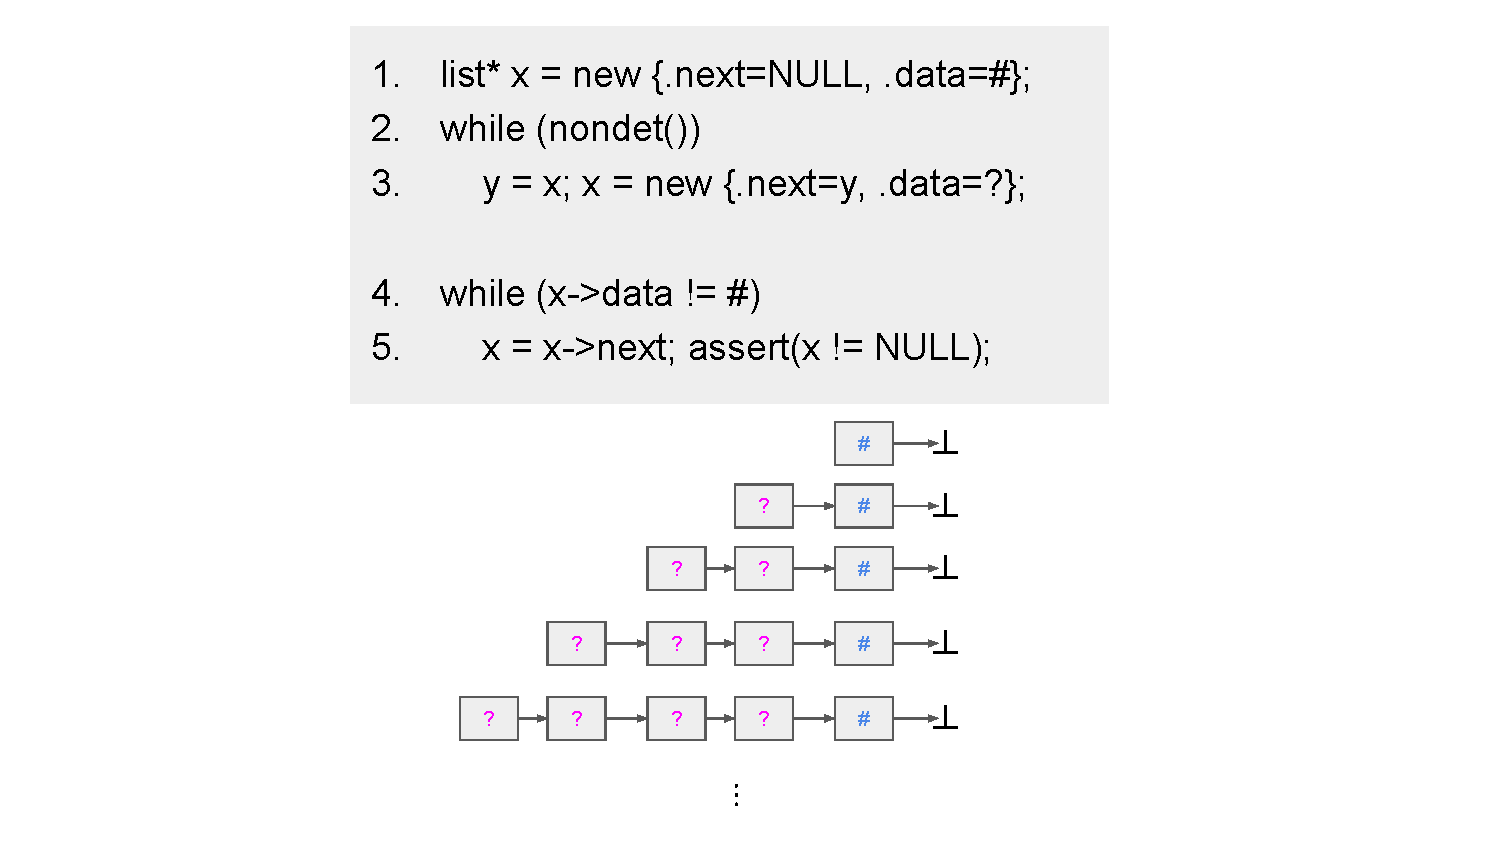
\includegraphics[scale=0.5]{ex/vmcai_1.pdf}}
       \only<2>{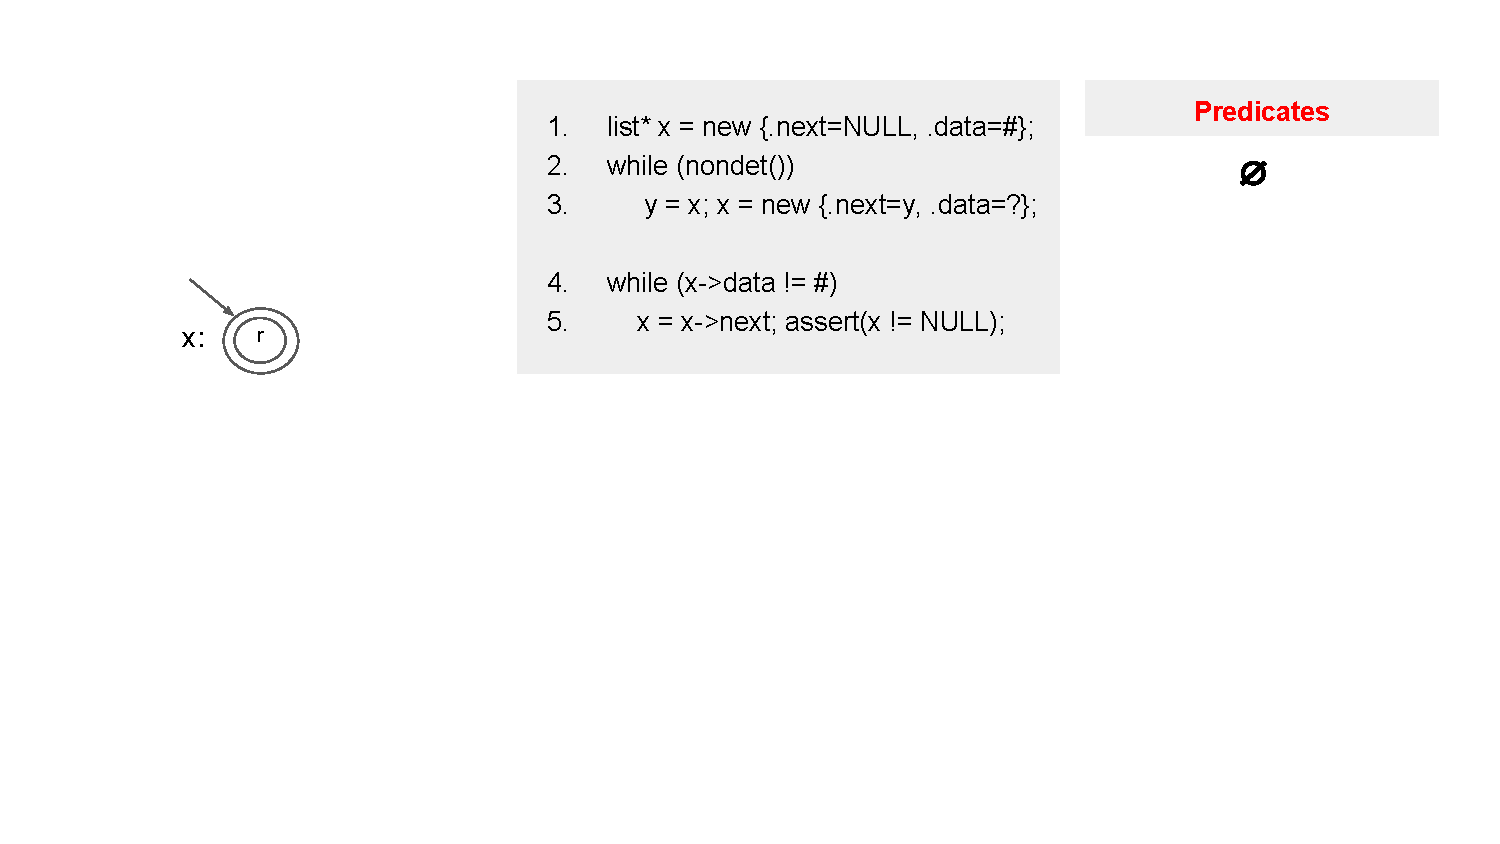
\includegraphics[scale=0.5]{ex/vmcai_2.pdf}}
       \only<3>{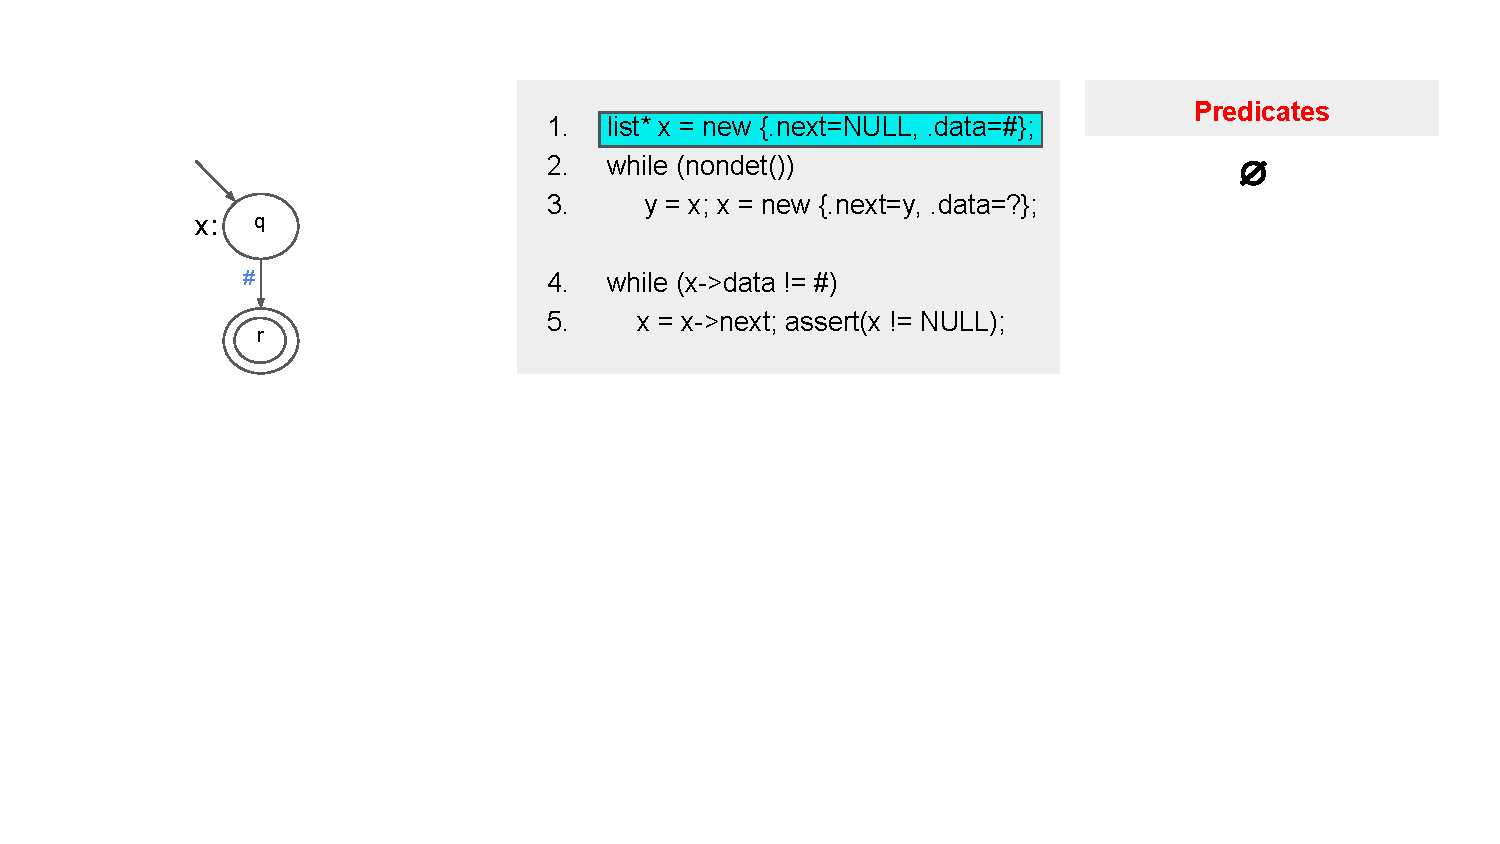
\includegraphics[scale=0.5]{ex/vmcai_3.pdf}}
       \only<4>{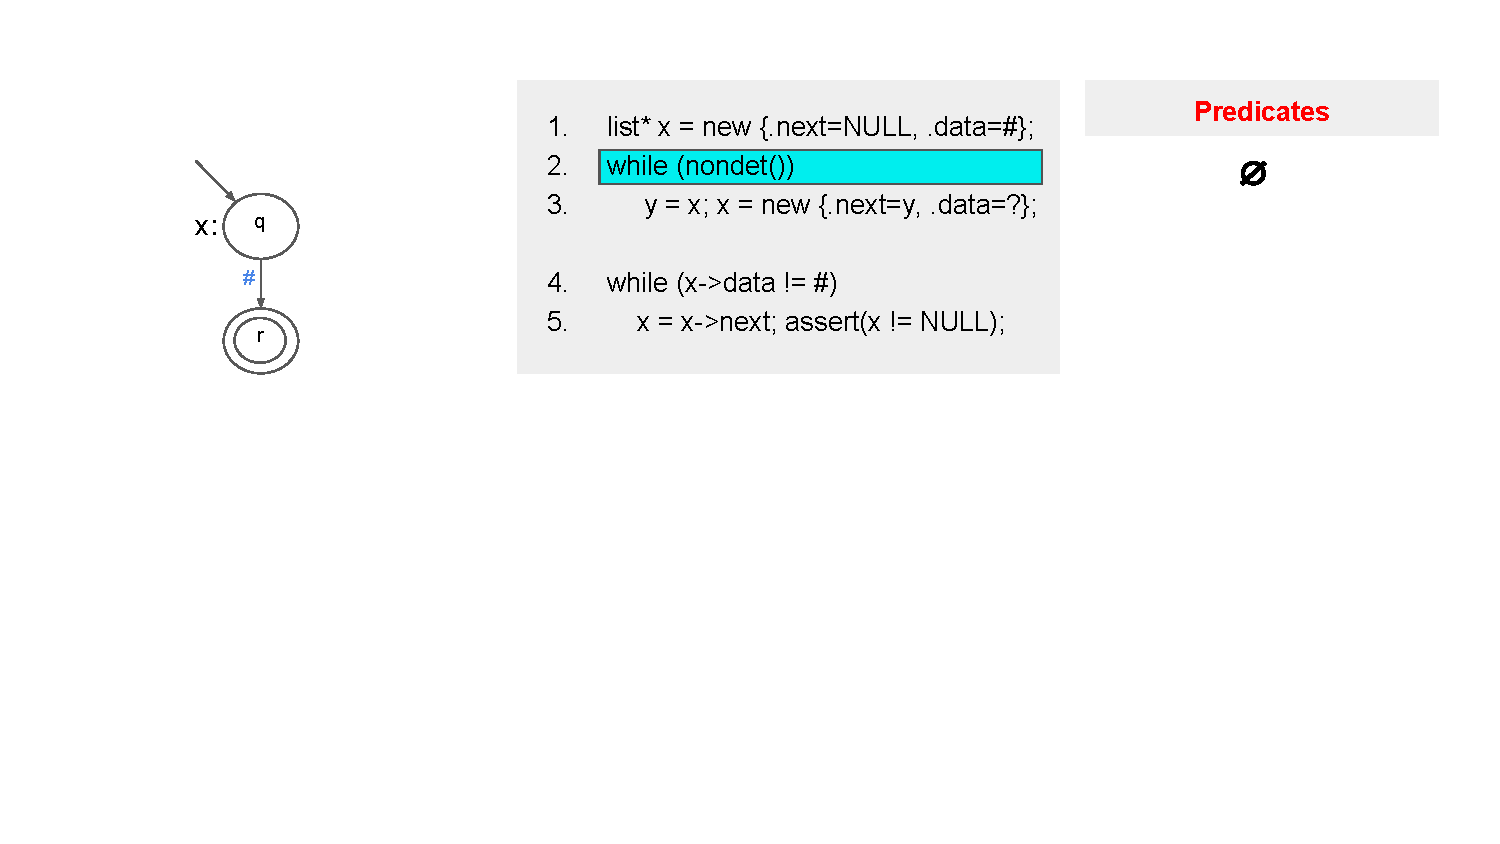
\includegraphics[scale=0.5]{ex/vmcai_4.pdf}}
       \only<5>{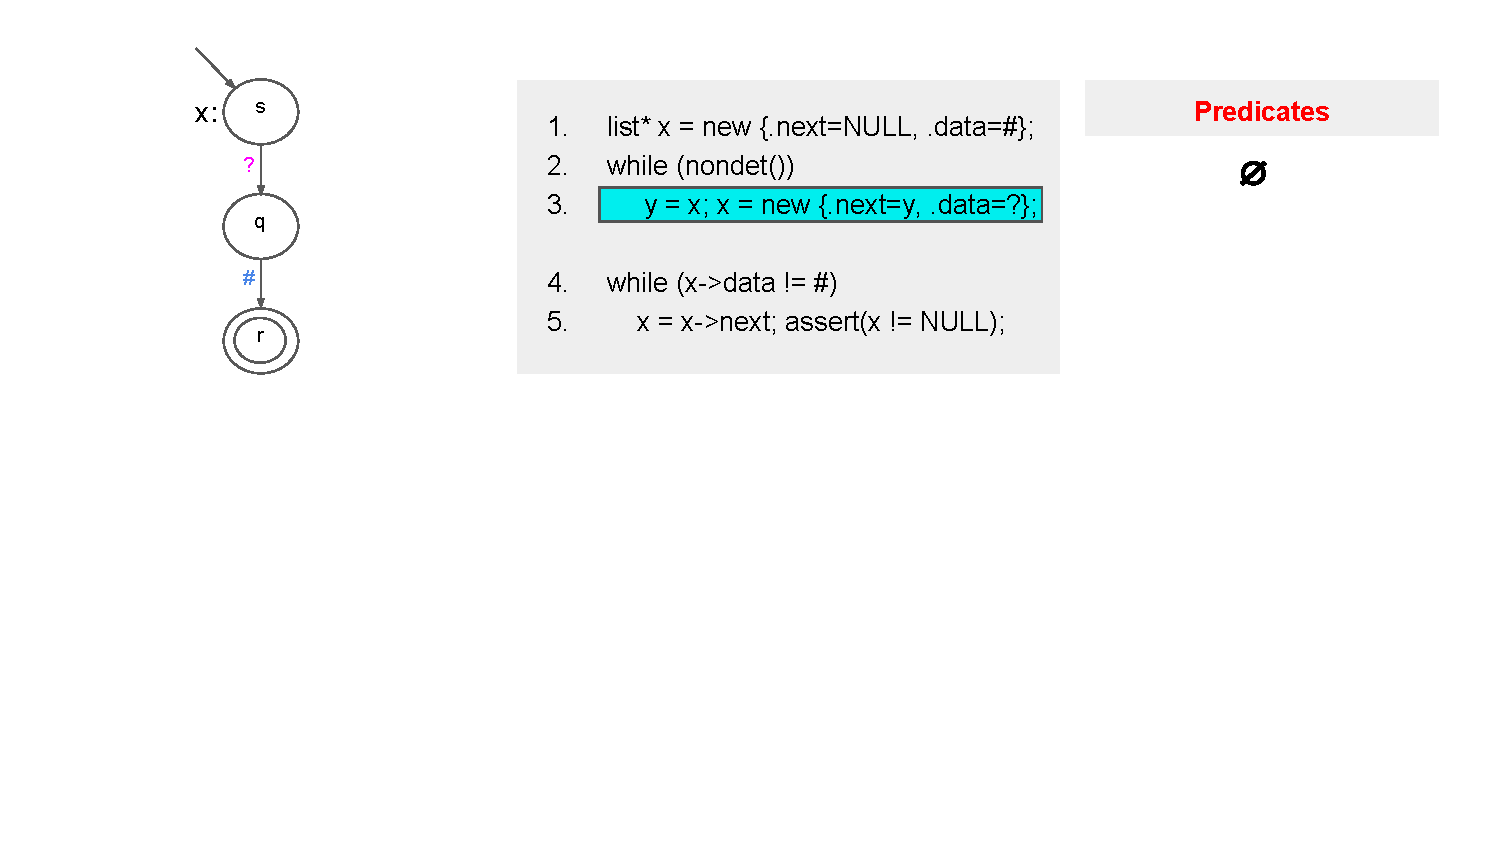
\includegraphics[scale=0.5]{ex/vmcai_5.pdf}}
       \only<6>{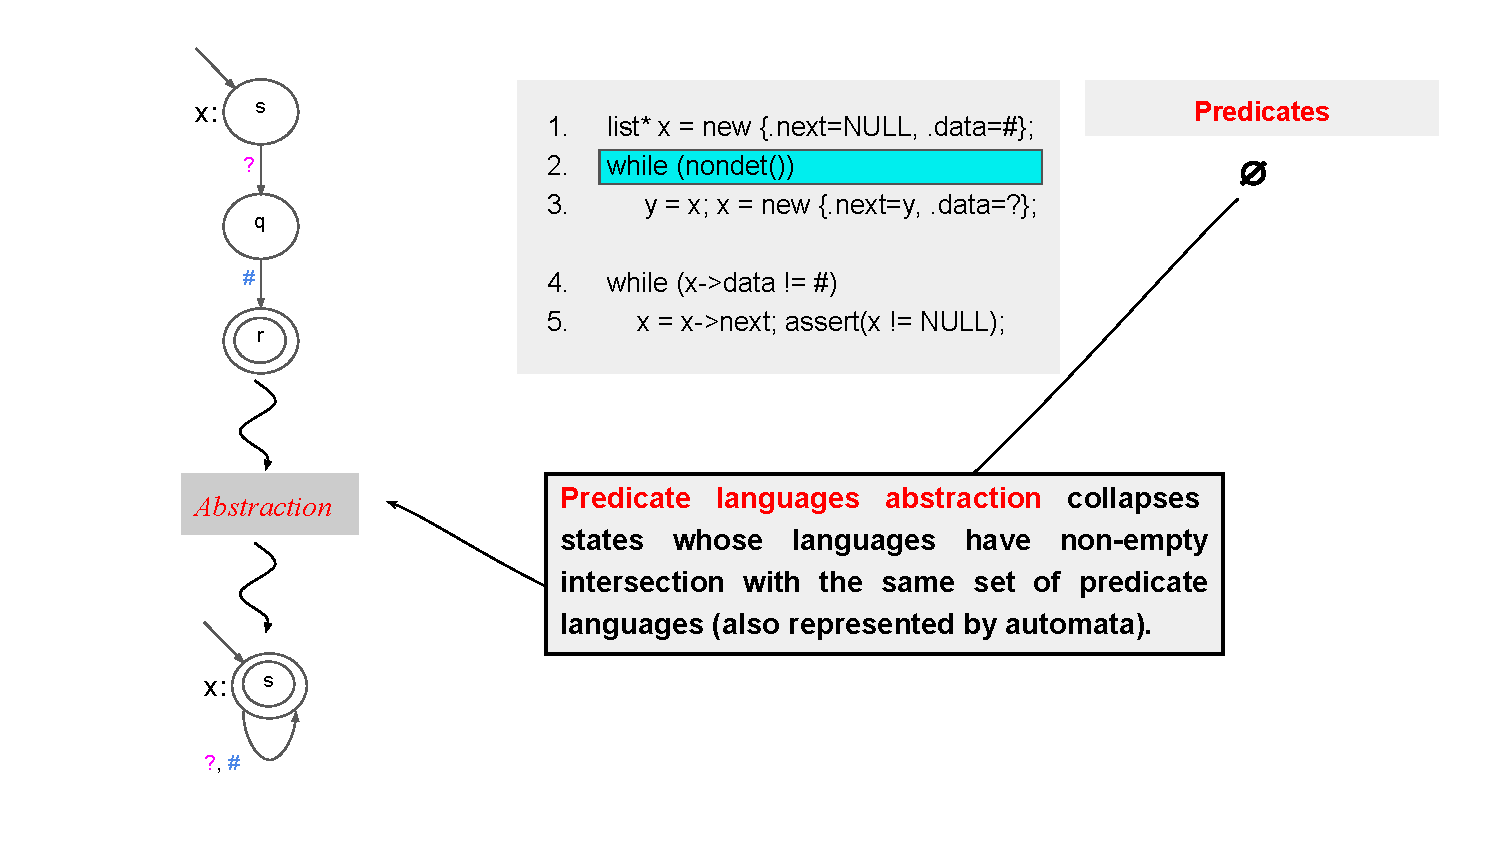
\includegraphics[scale=0.5]{ex/vmcai_6.pdf}}
       \only<7>{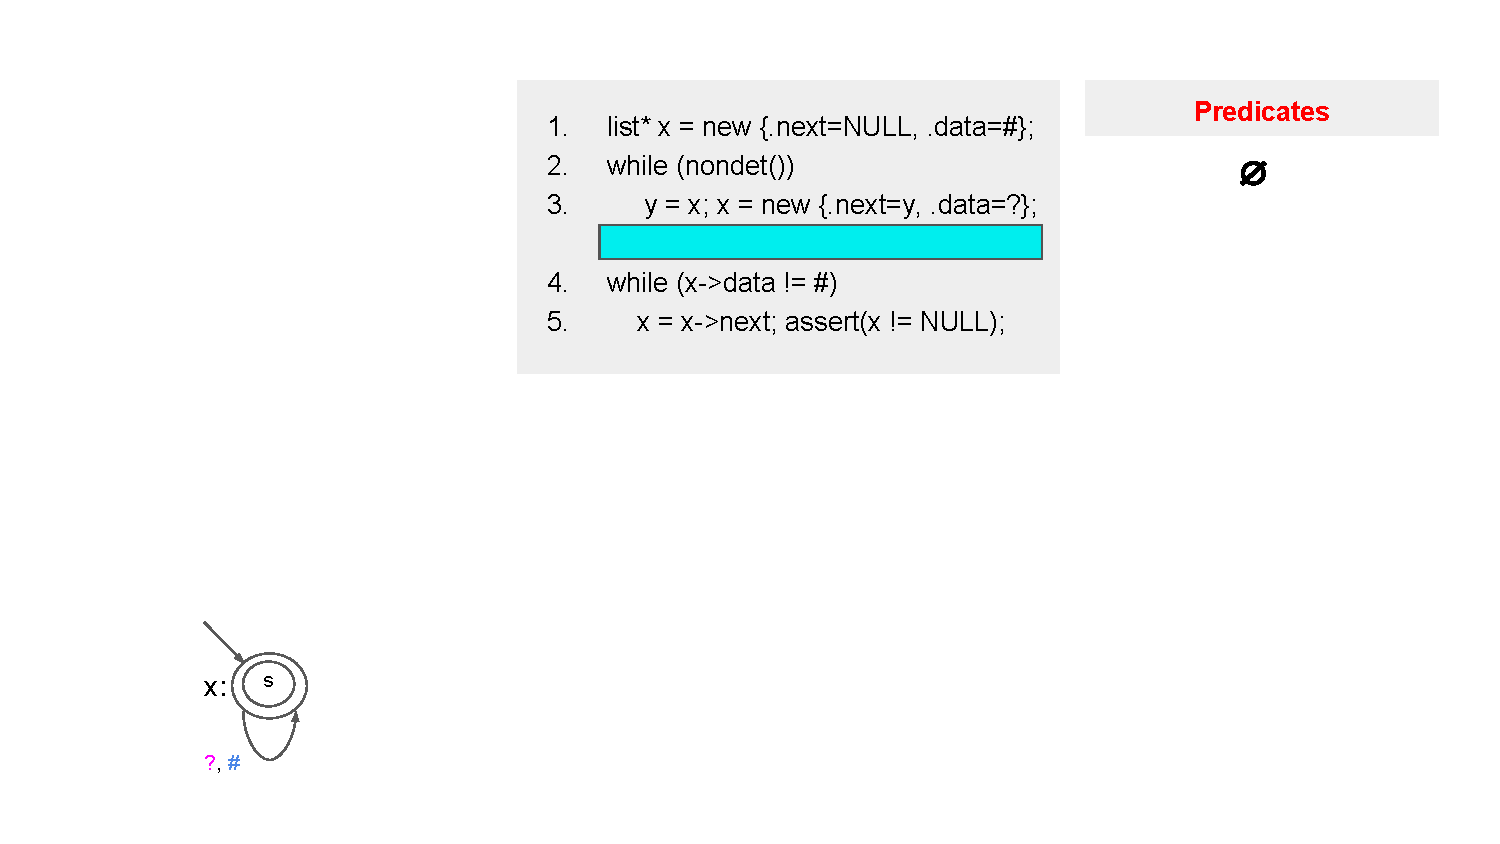
\includegraphics[scale=0.5]{ex/vmcai_7.pdf}}
       \only<8>{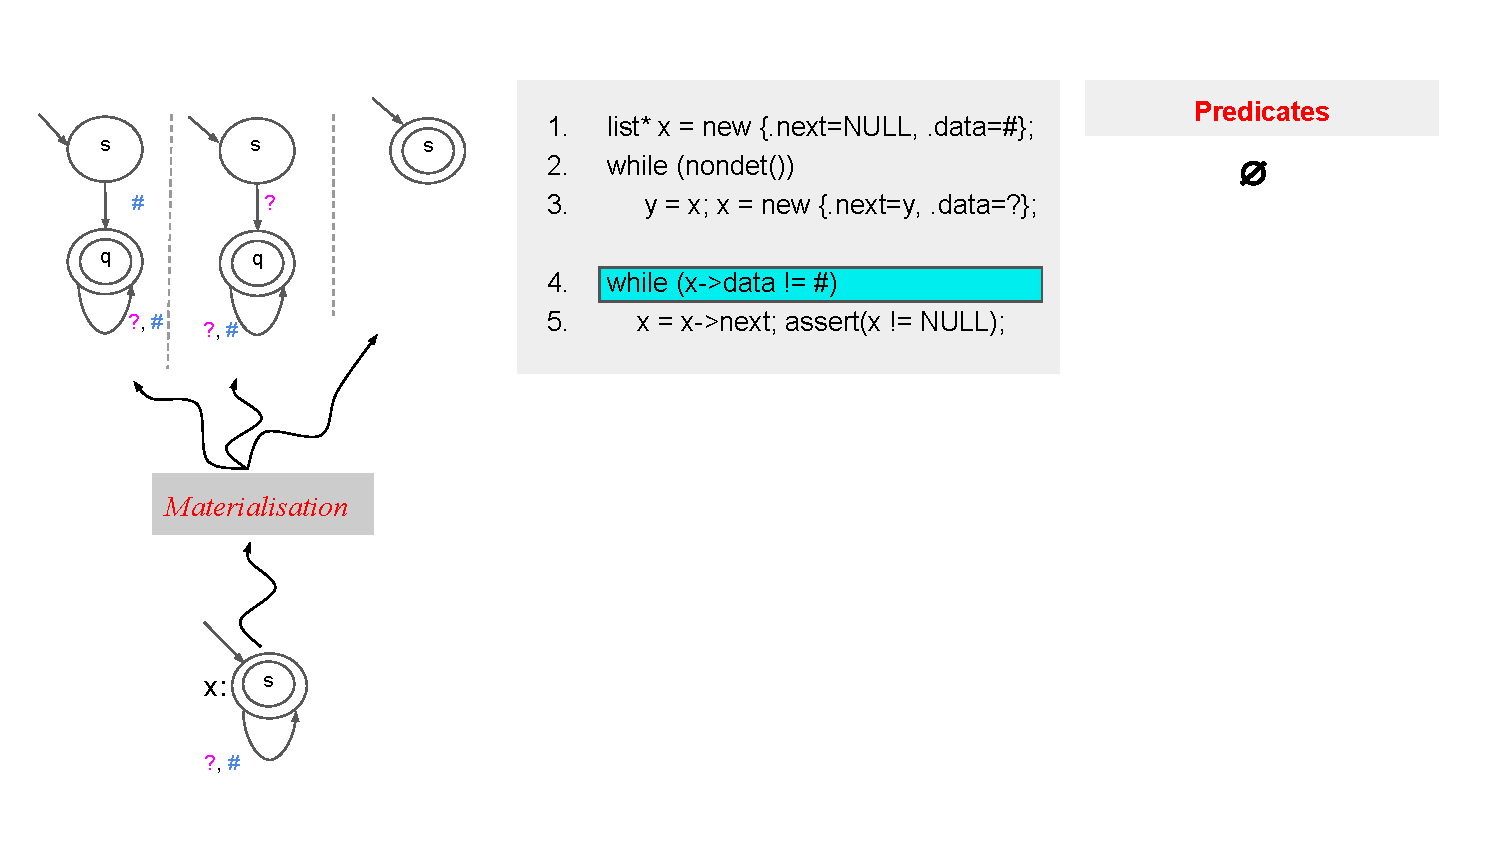
\includegraphics[scale=0.5]{ex/vmcai_8.pdf}}
       \only<9>{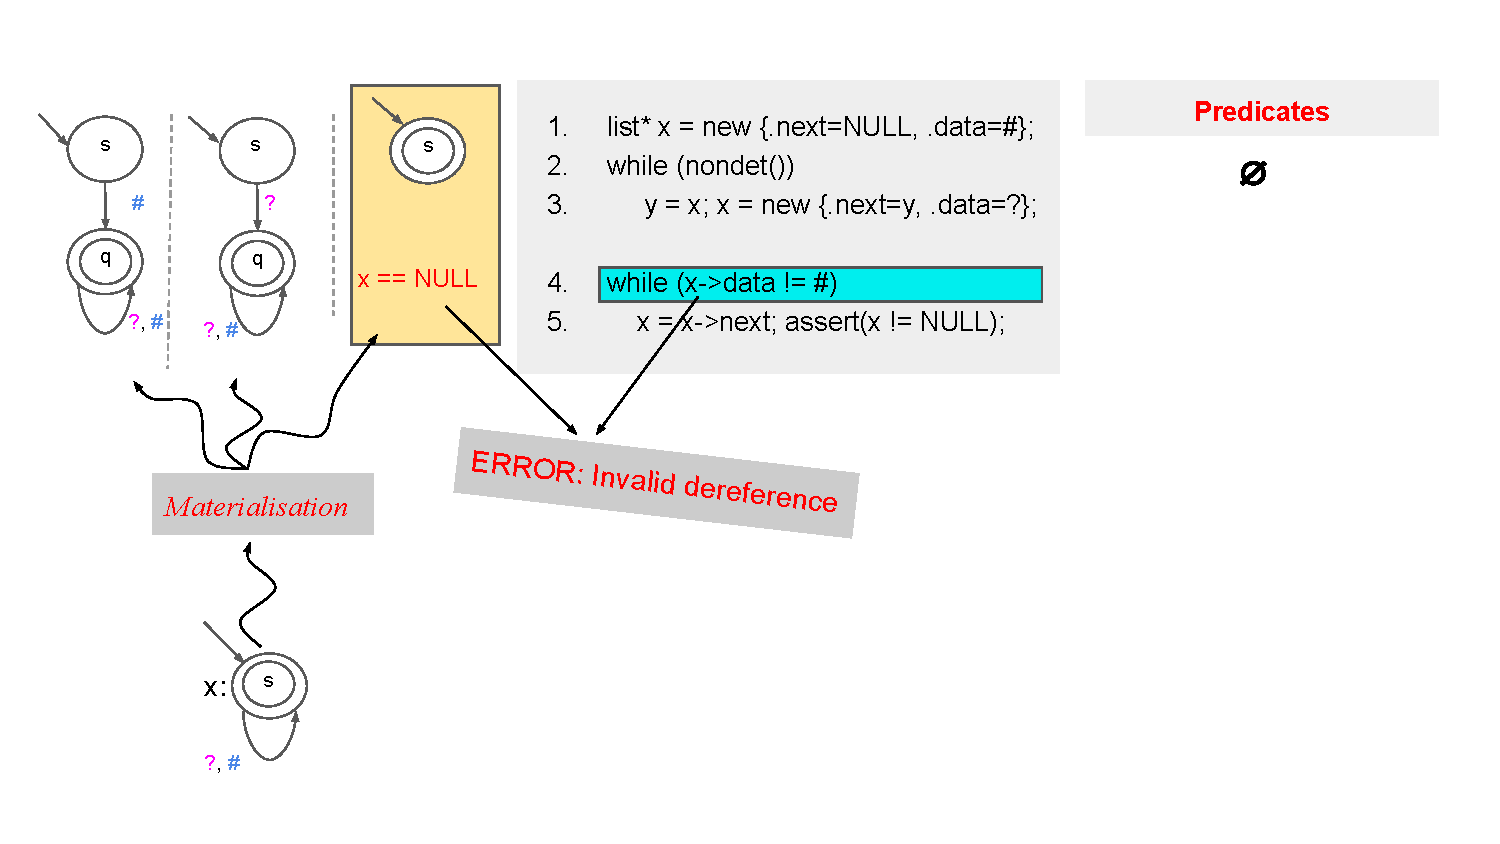
\includegraphics[scale=0.5]{ex/vmcai_9.pdf}}
     \end{overlayarea}
 \end{frame}
 
% %*******************************************************************************
% 
% %*******************************************************************************
 \begin{frame}[noframenumbering]
 % \begin{frame}[label=current]
   \frametitle{Example\,---\,Backward Run}
   \begin{overlayarea}{7cm}{6.5cm}
       \only<1>{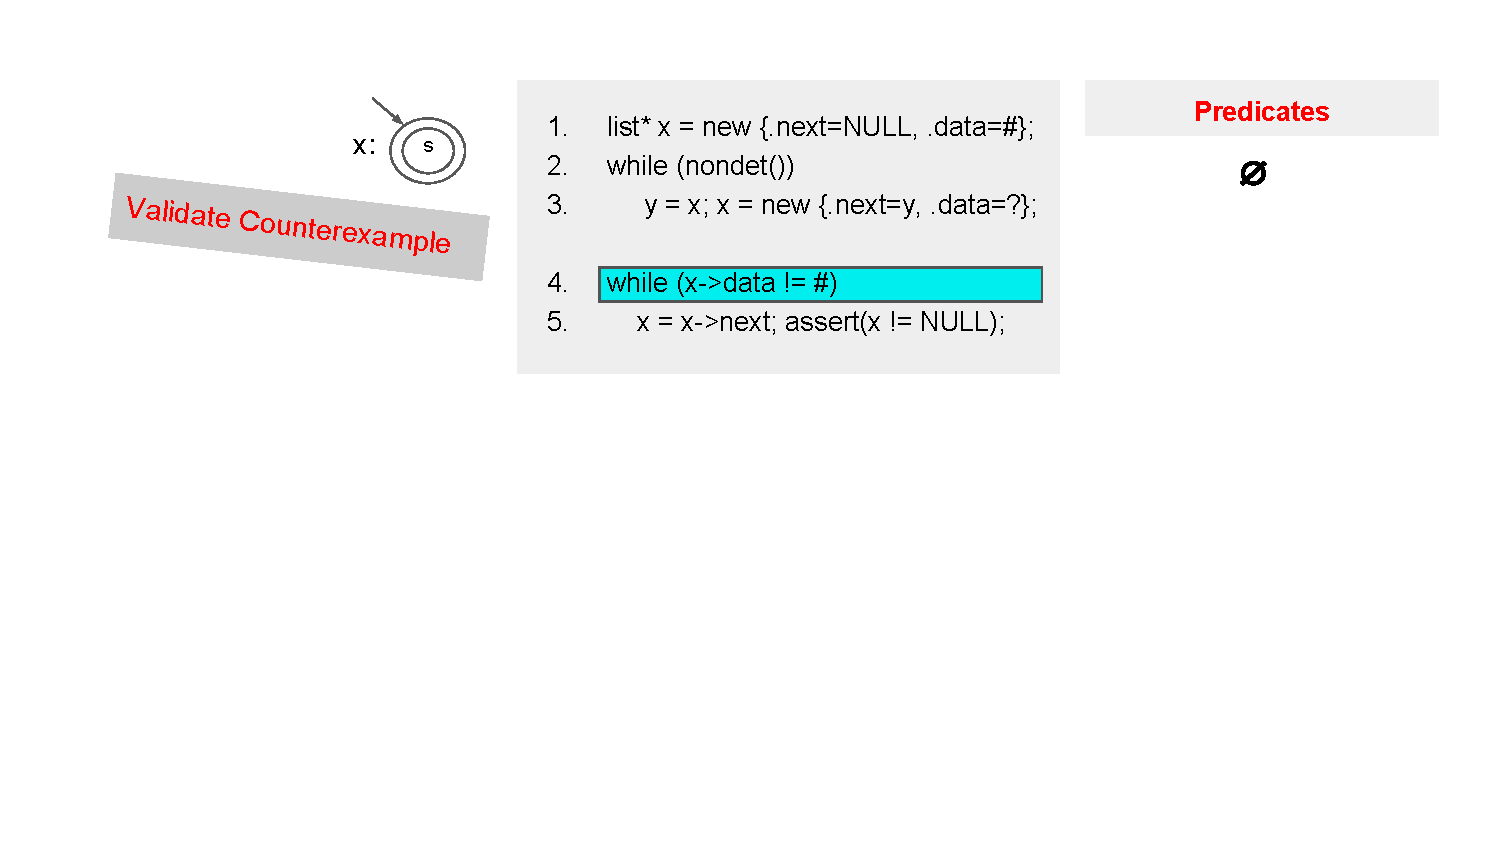
\includegraphics[scale=0.5]{ex/vmcai_10.pdf}}
       \only<2>{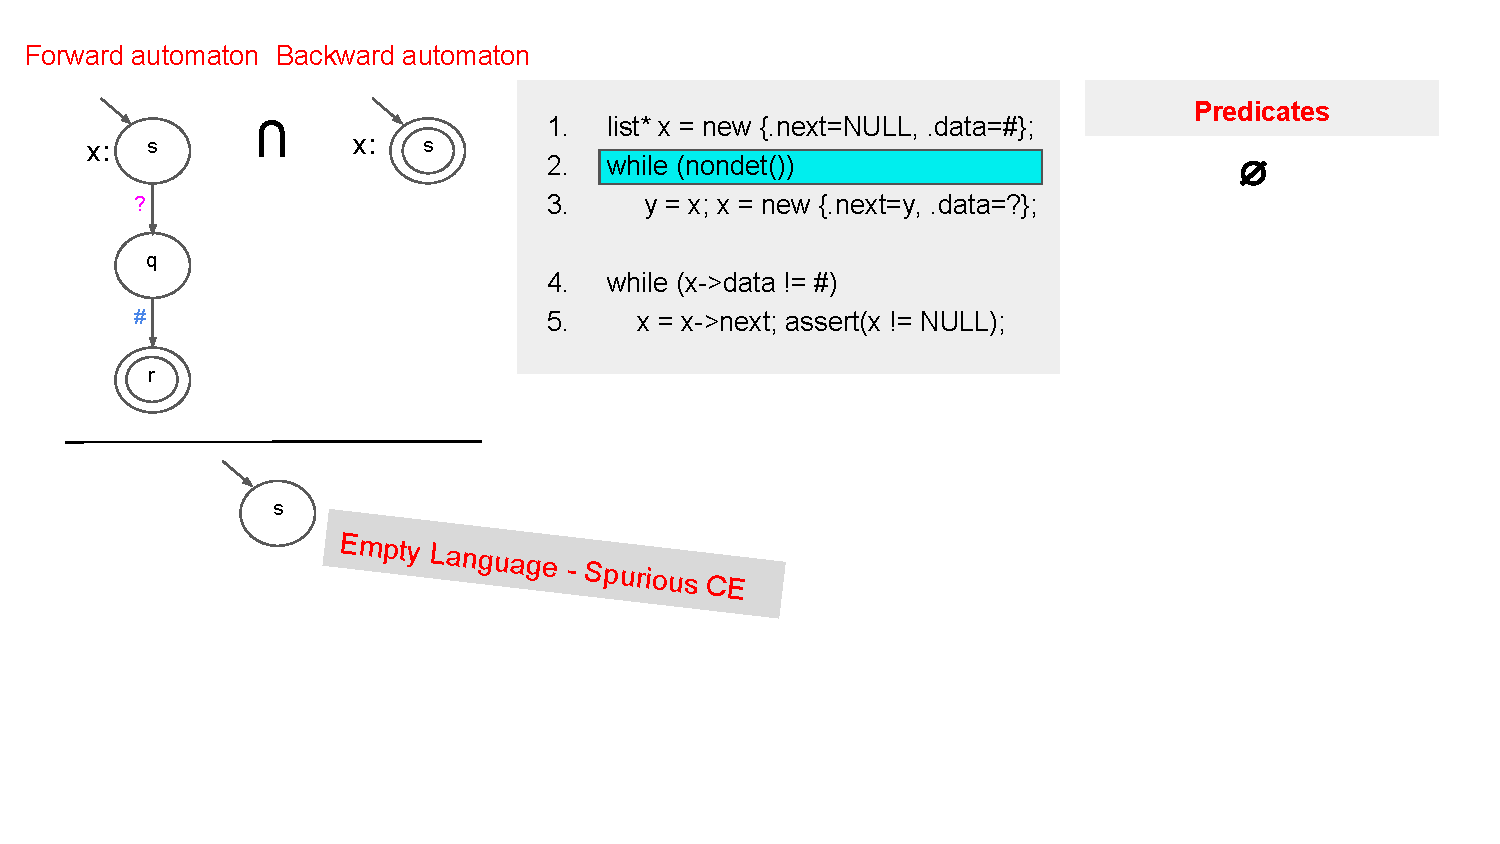
\includegraphics[scale=0.5]{ex/vmcai_11.pdf}}
       \only<3>{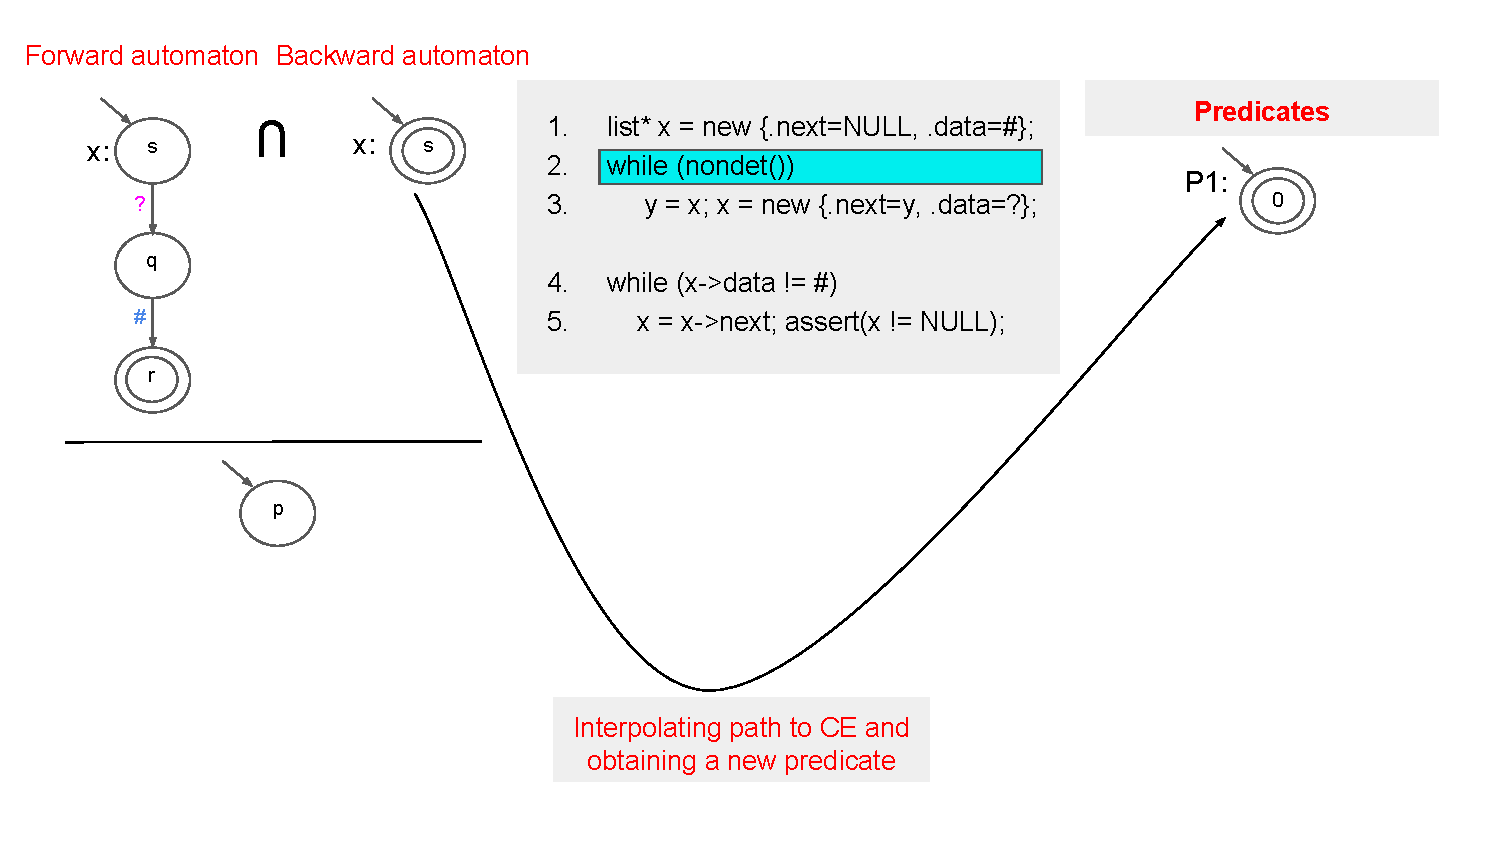
\includegraphics[scale=0.5]{ex/vmcai_12.pdf}}
   \end{overlayarea}
 \end{frame}

%%*******************************************************************************
%
%%*******************************************************************************
 \begin{frame}[noframenumbering]
 % \begin{frame}[label=current]
   \frametitle{Example\,---\,Forward Run no. 2}
   \begin{overlayarea}{7cm}{6.5cm}
       \only<1>{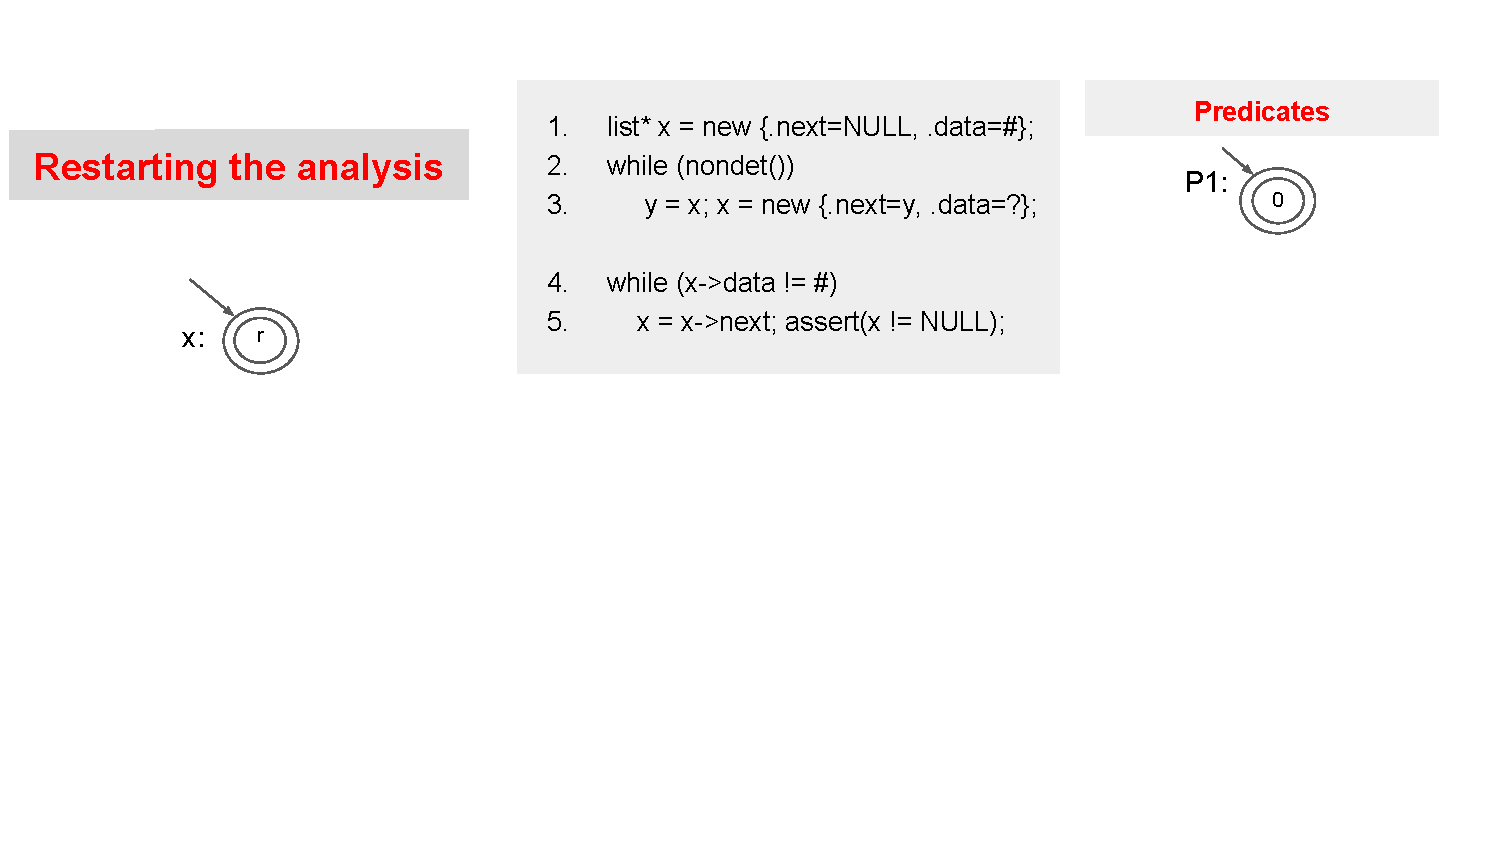
\includegraphics[scale=0.5]{ex/vmcai_13.pdf}}
       \only<2>{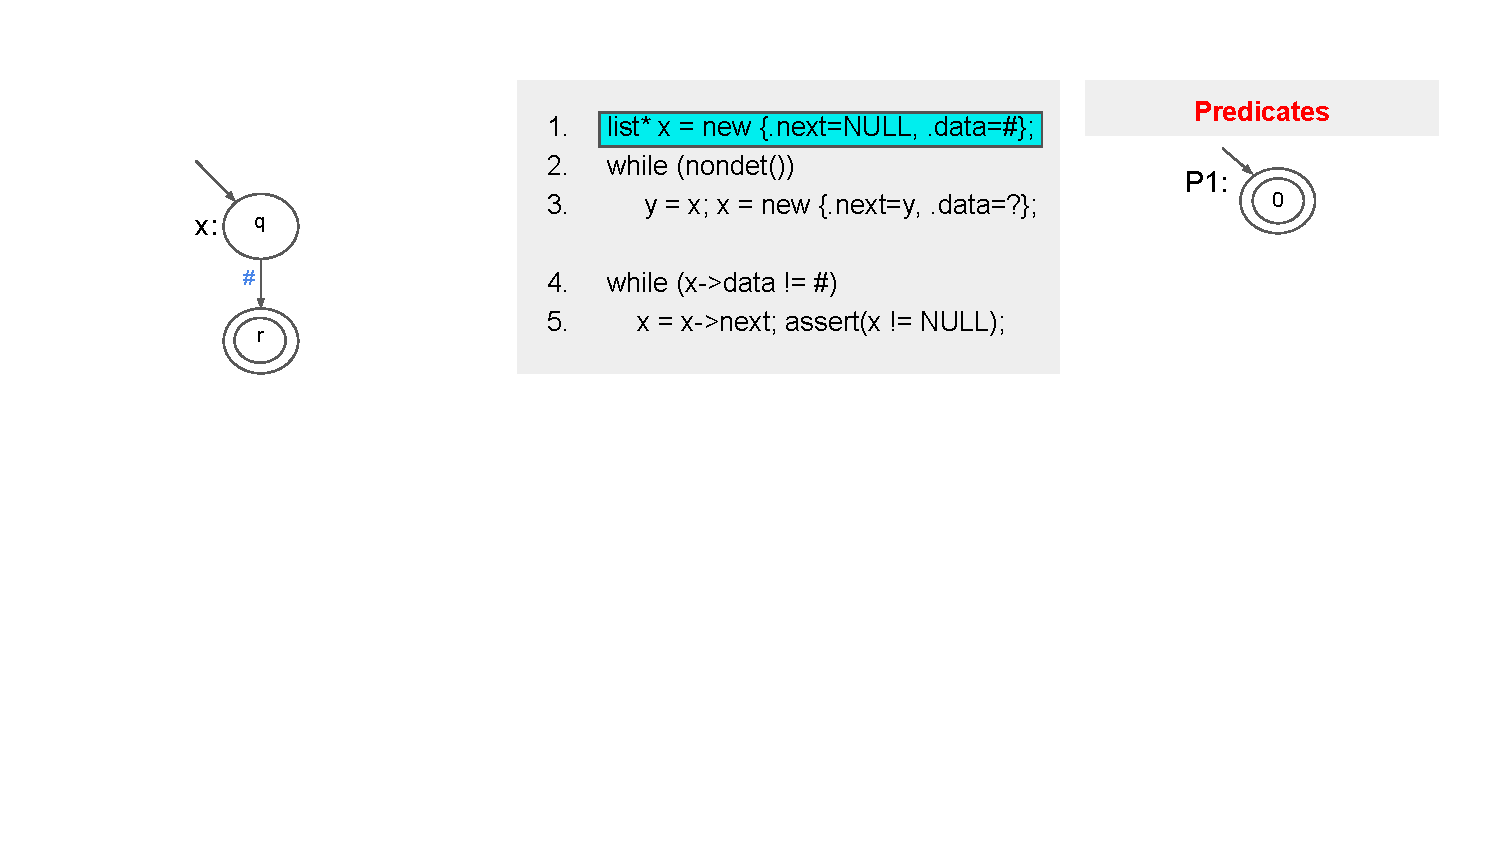
\includegraphics[scale=0.5]{ex/vmcai_14.pdf}}
       \only<3>{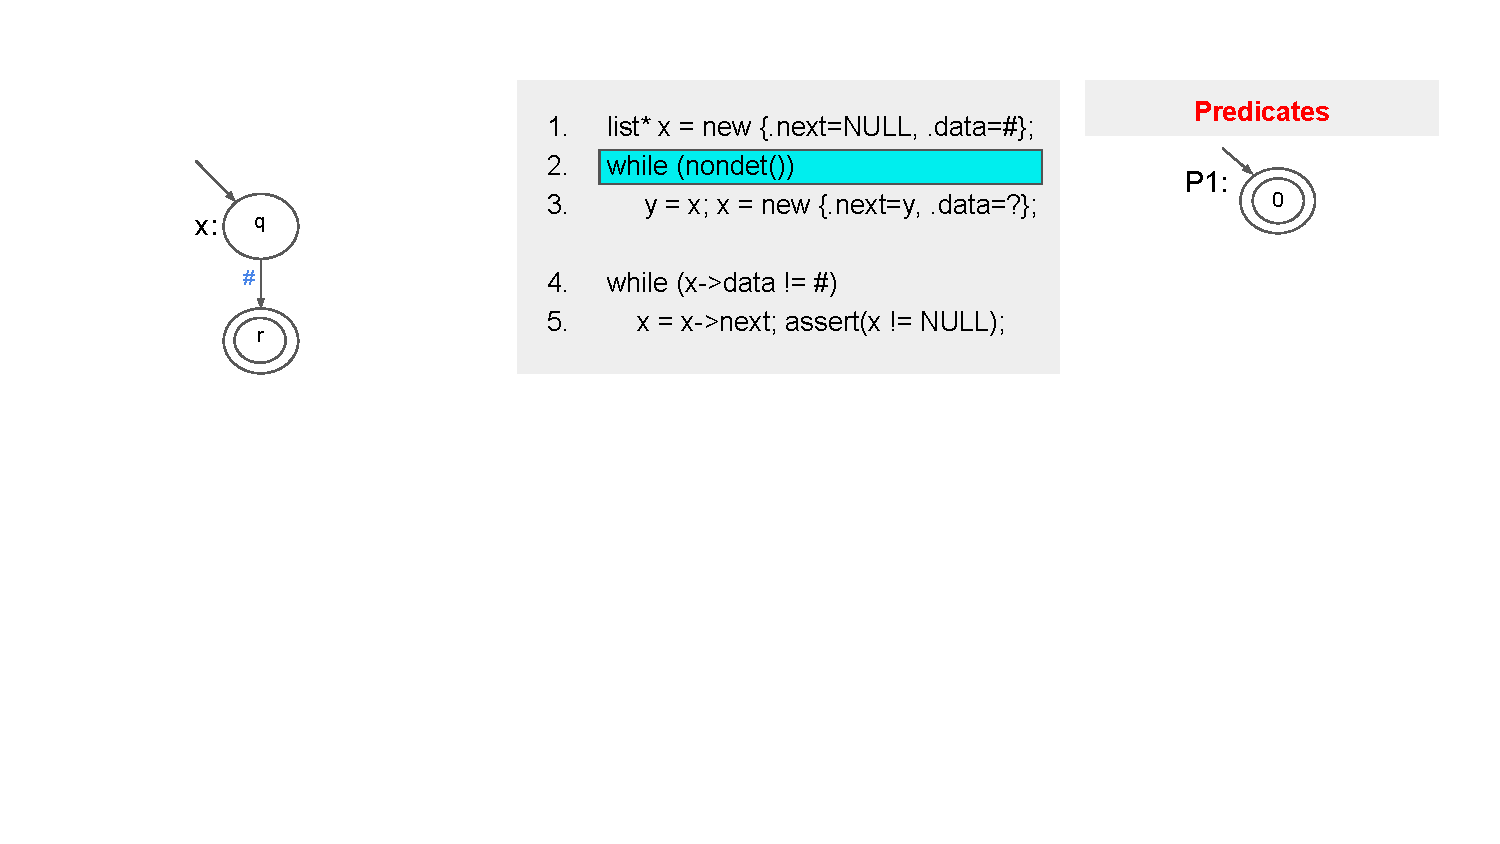
\includegraphics[scale=0.5]{ex/vmcai_15.pdf}}
       \only<4>{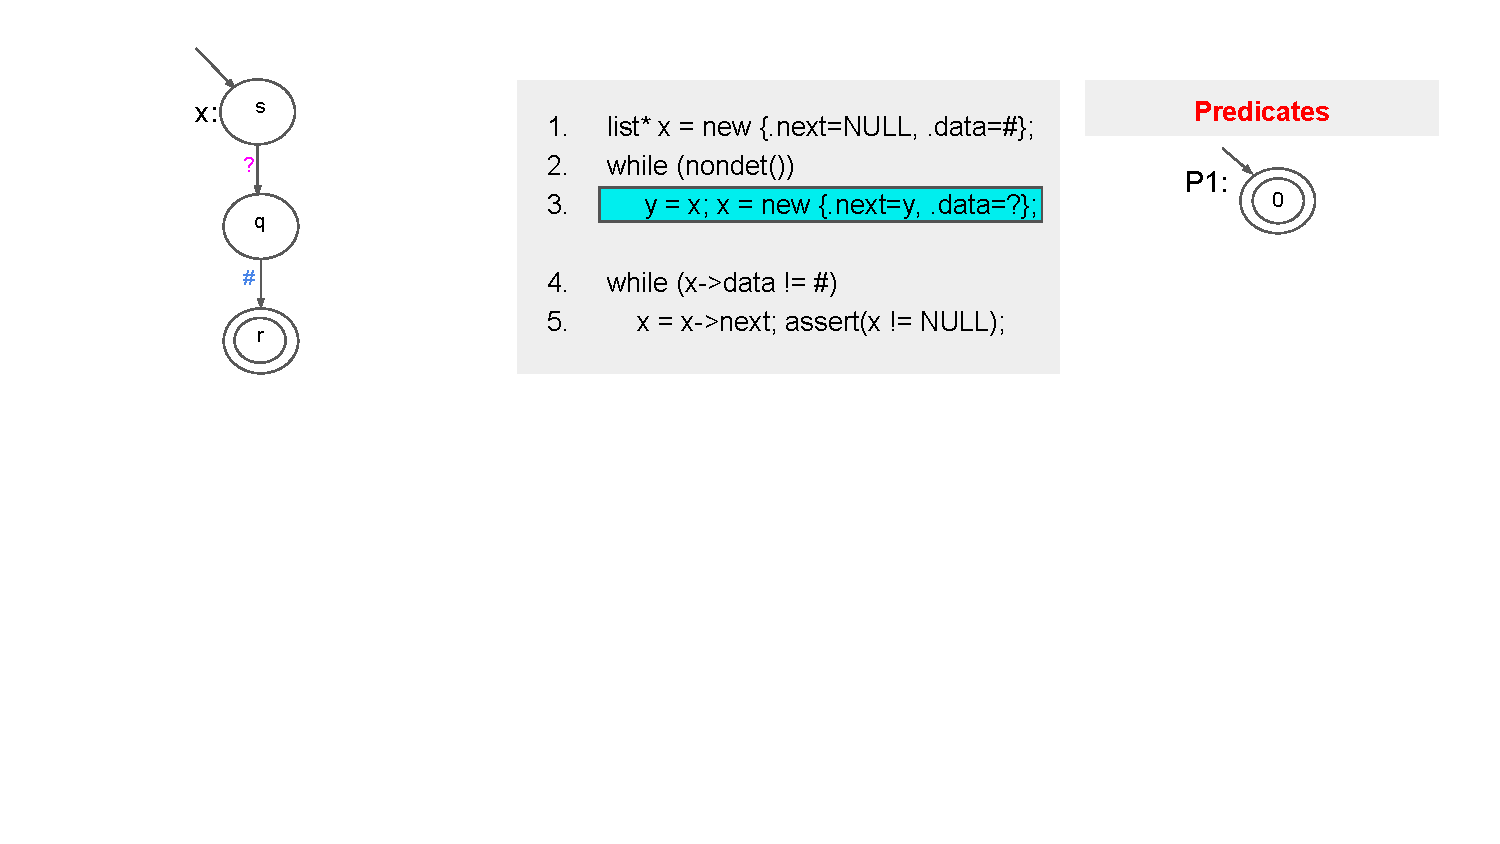
\includegraphics[scale=0.5]{ex/vmcai_16.pdf}}
       \only<5>{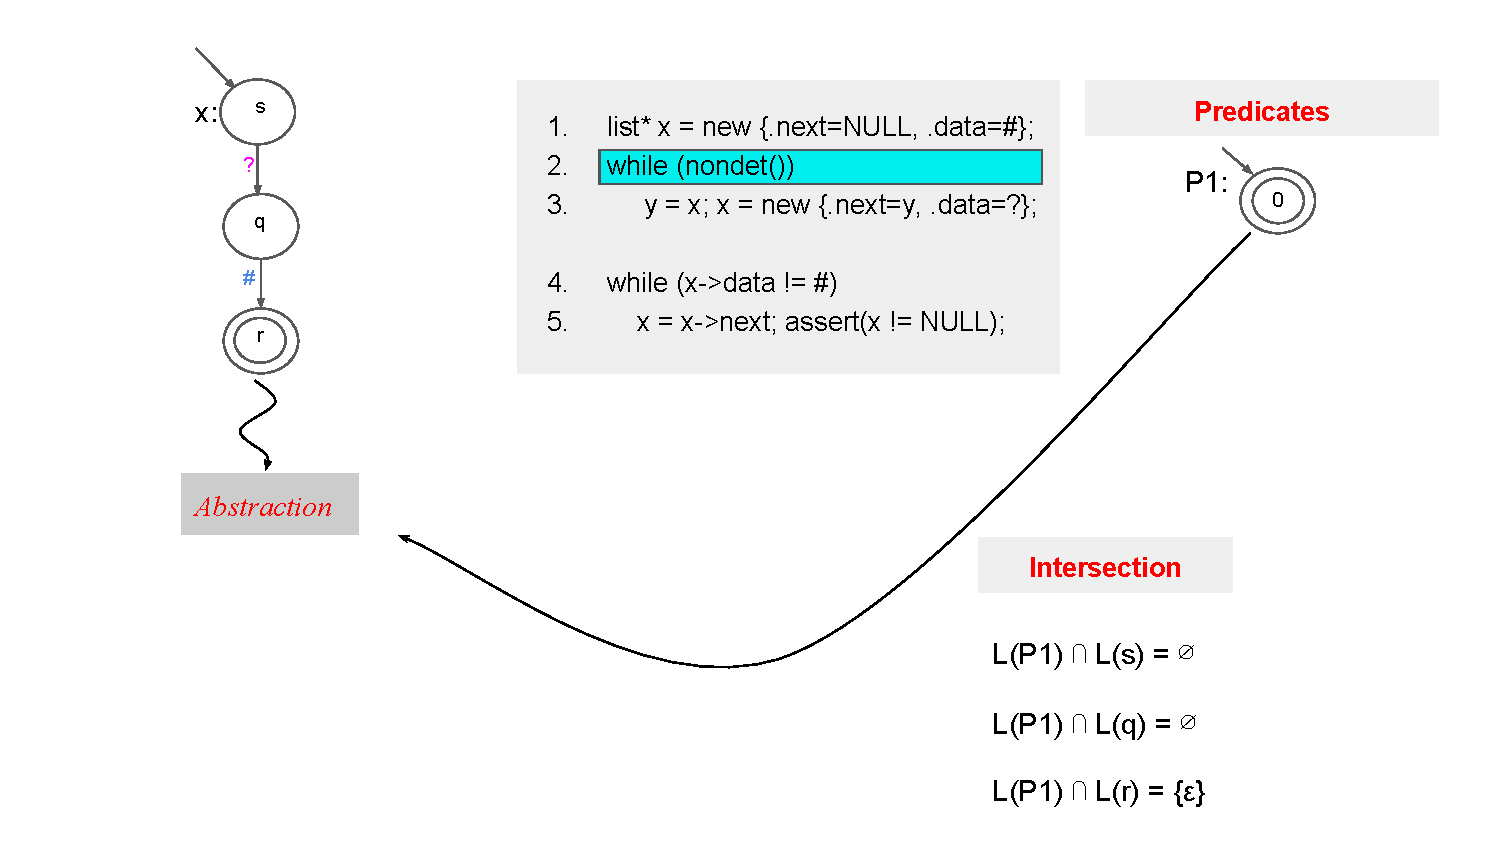
\includegraphics[scale=0.5]{ex/vmcai_17.pdf}}
       \only<6>{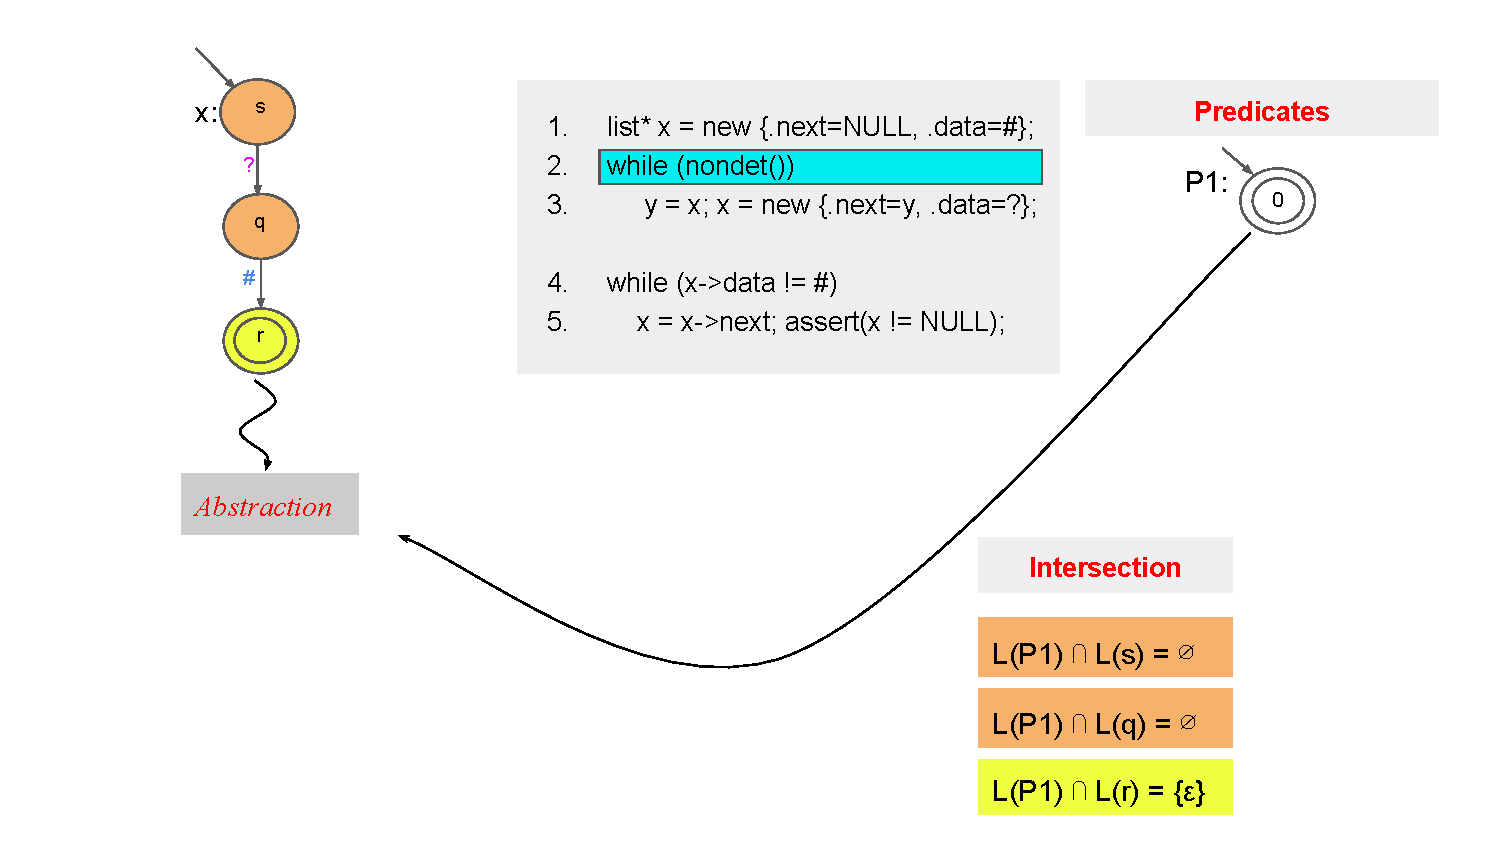
\includegraphics[scale=0.5]{ex/vmcai_18.pdf}}
       \only<7>{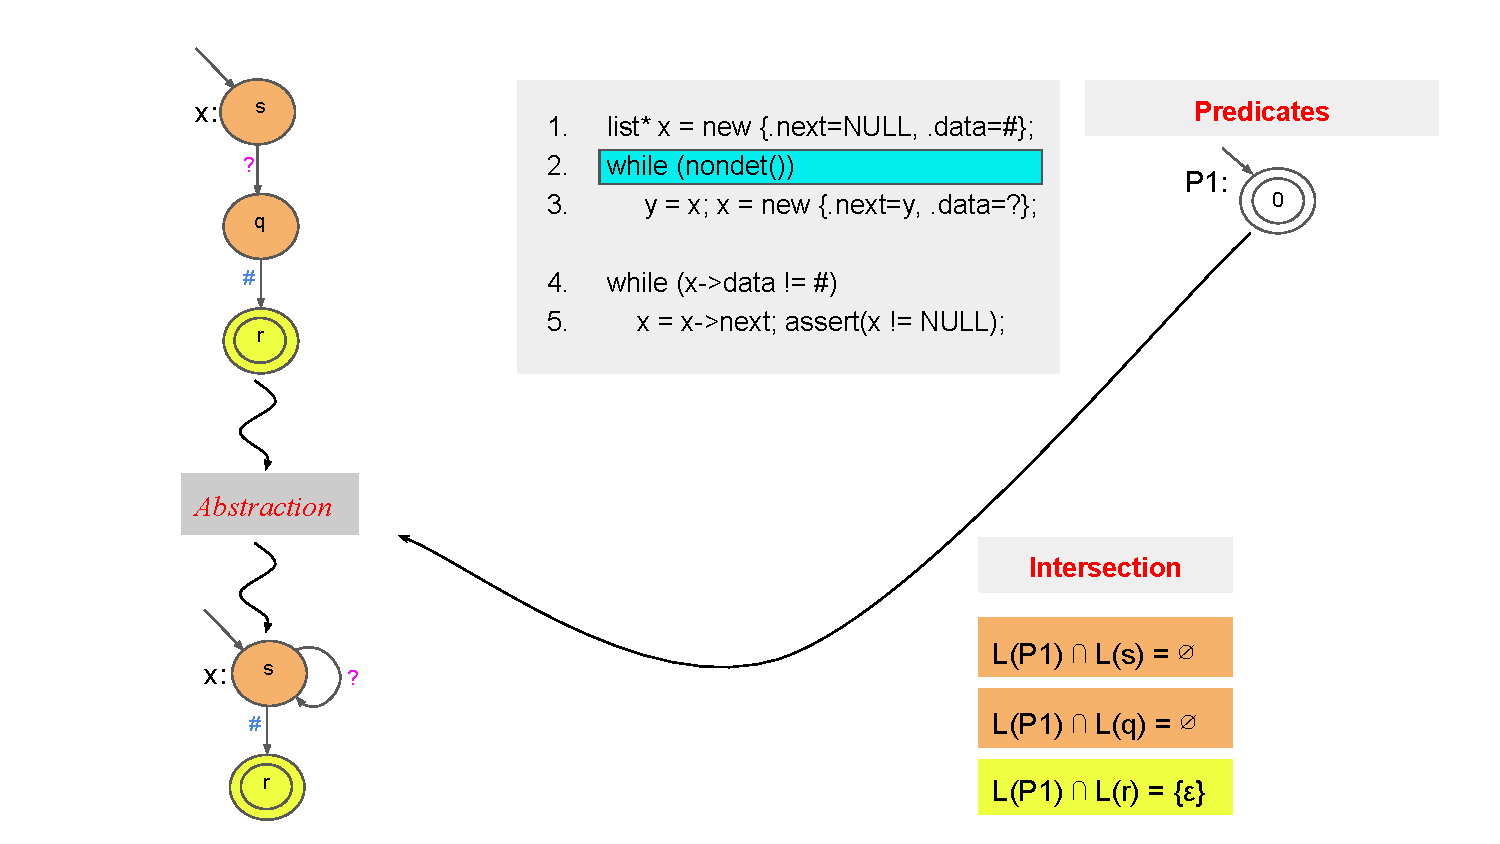
\includegraphics[scale=0.5]{ex/vmcai_19.pdf}}
 	  \only<8>{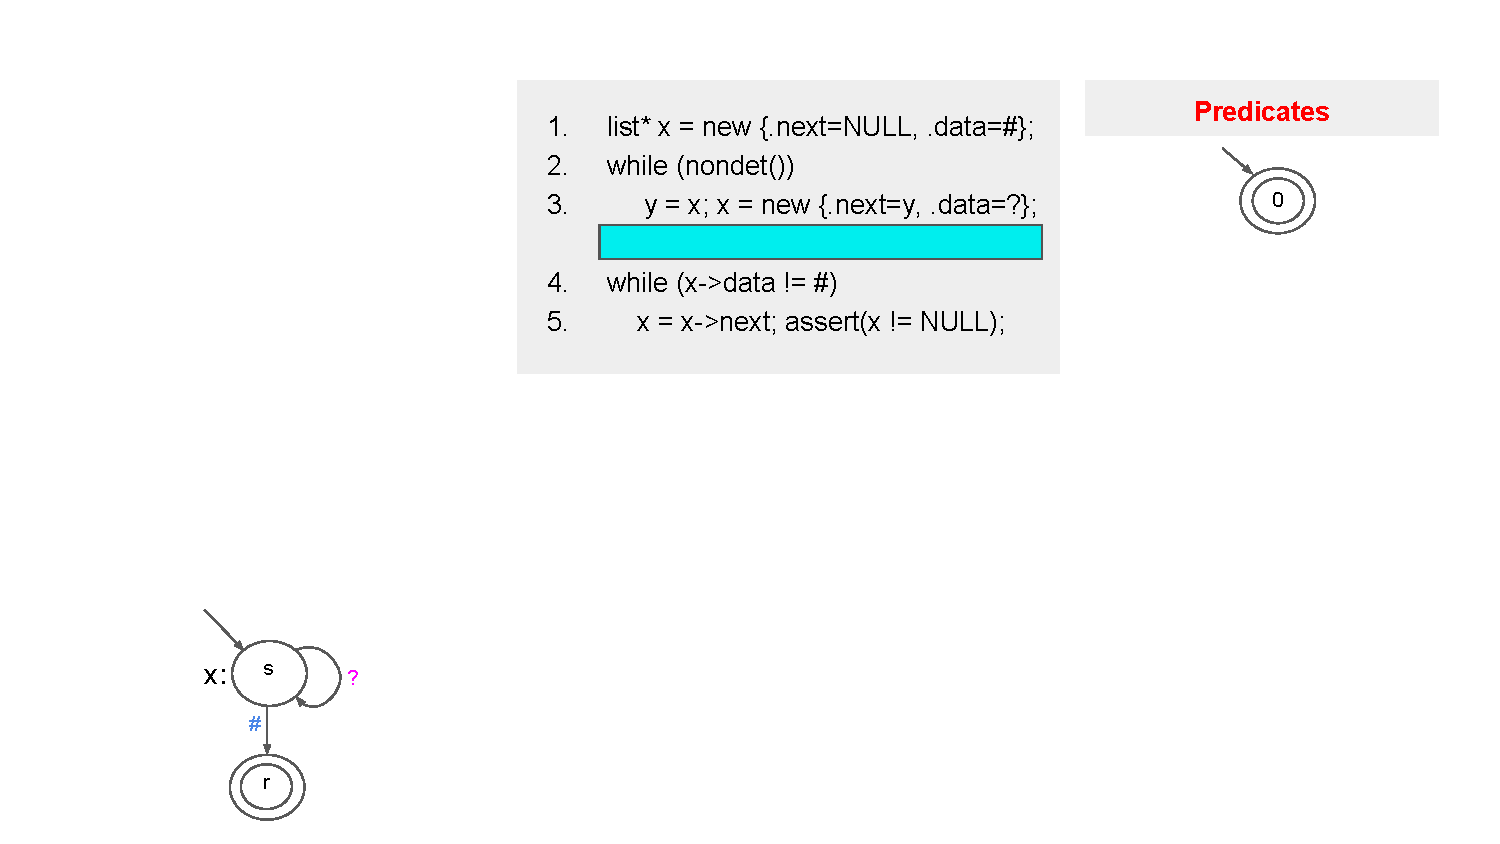
\includegraphics[scale=0.5]{ex/vmcai_20.pdf}}
 	  \only<9>{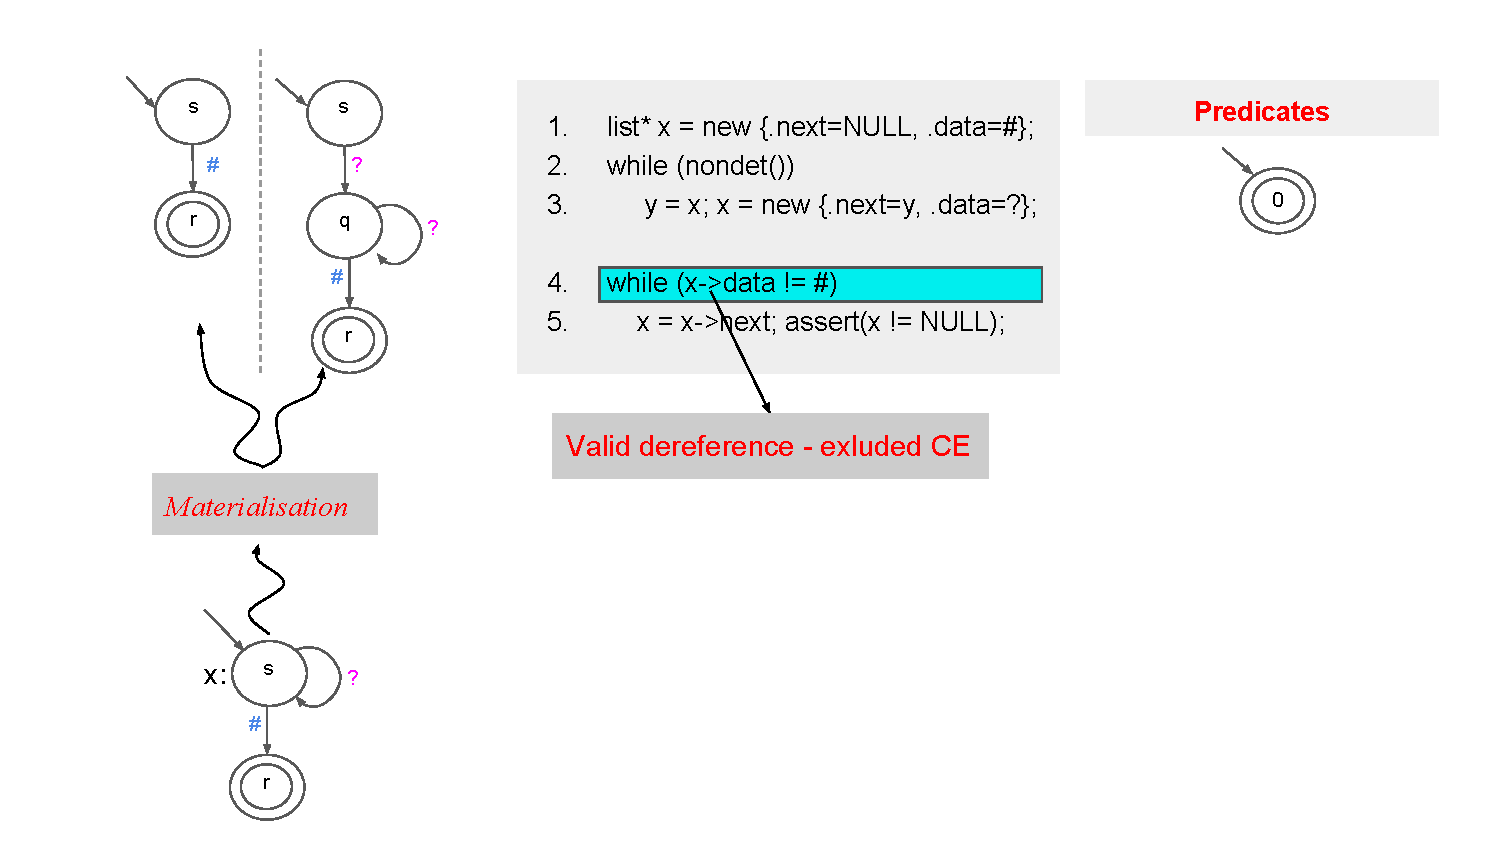
\includegraphics[scale=0.5]{ex/vmcai_21.pdf}}
       \only<10>{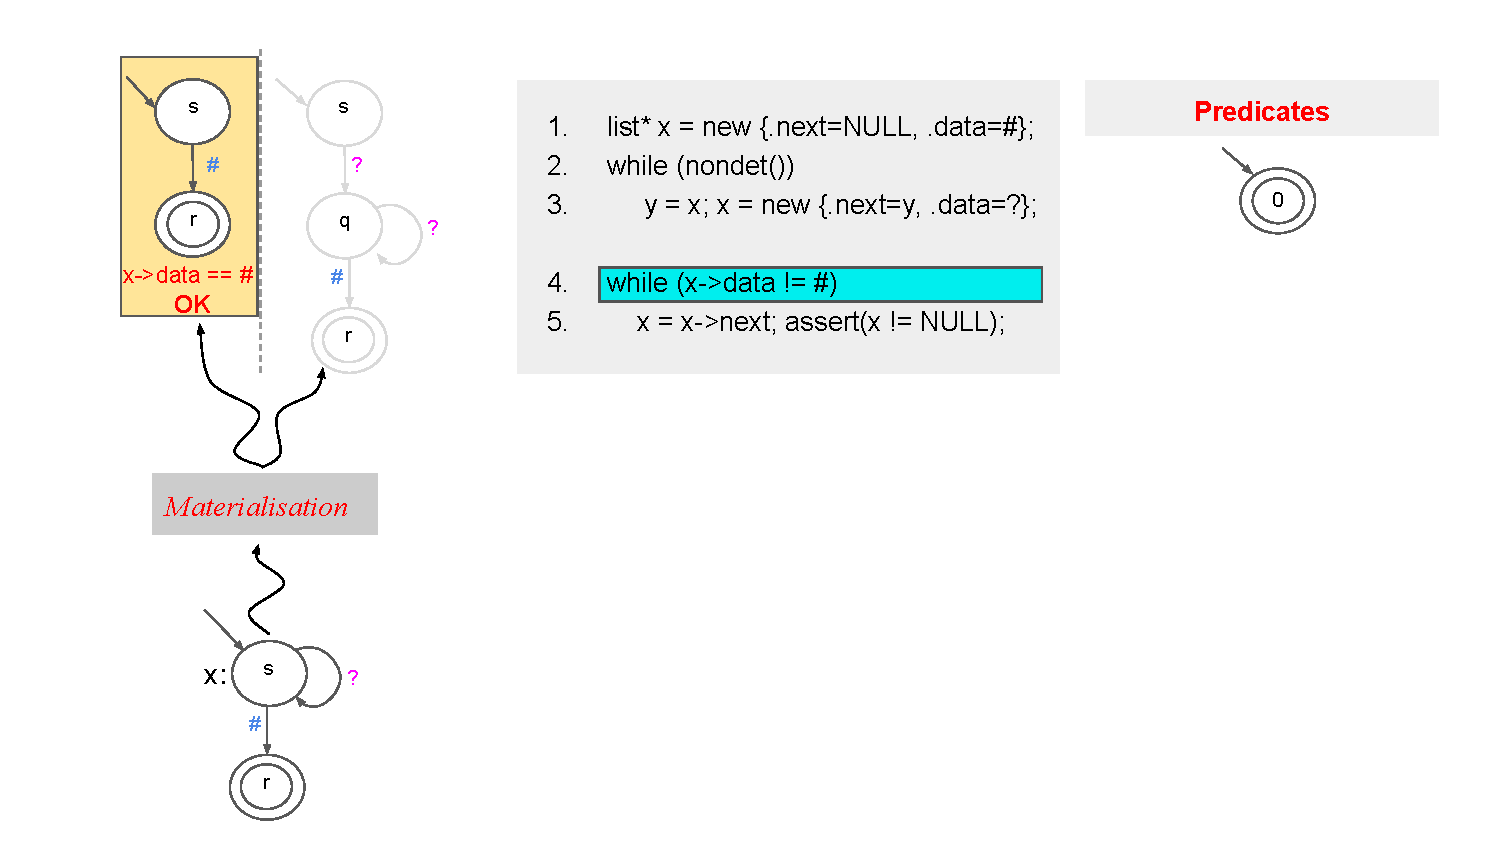
\includegraphics[scale=0.5]{ex/vmcai_22.pdf}}
       \only<11>{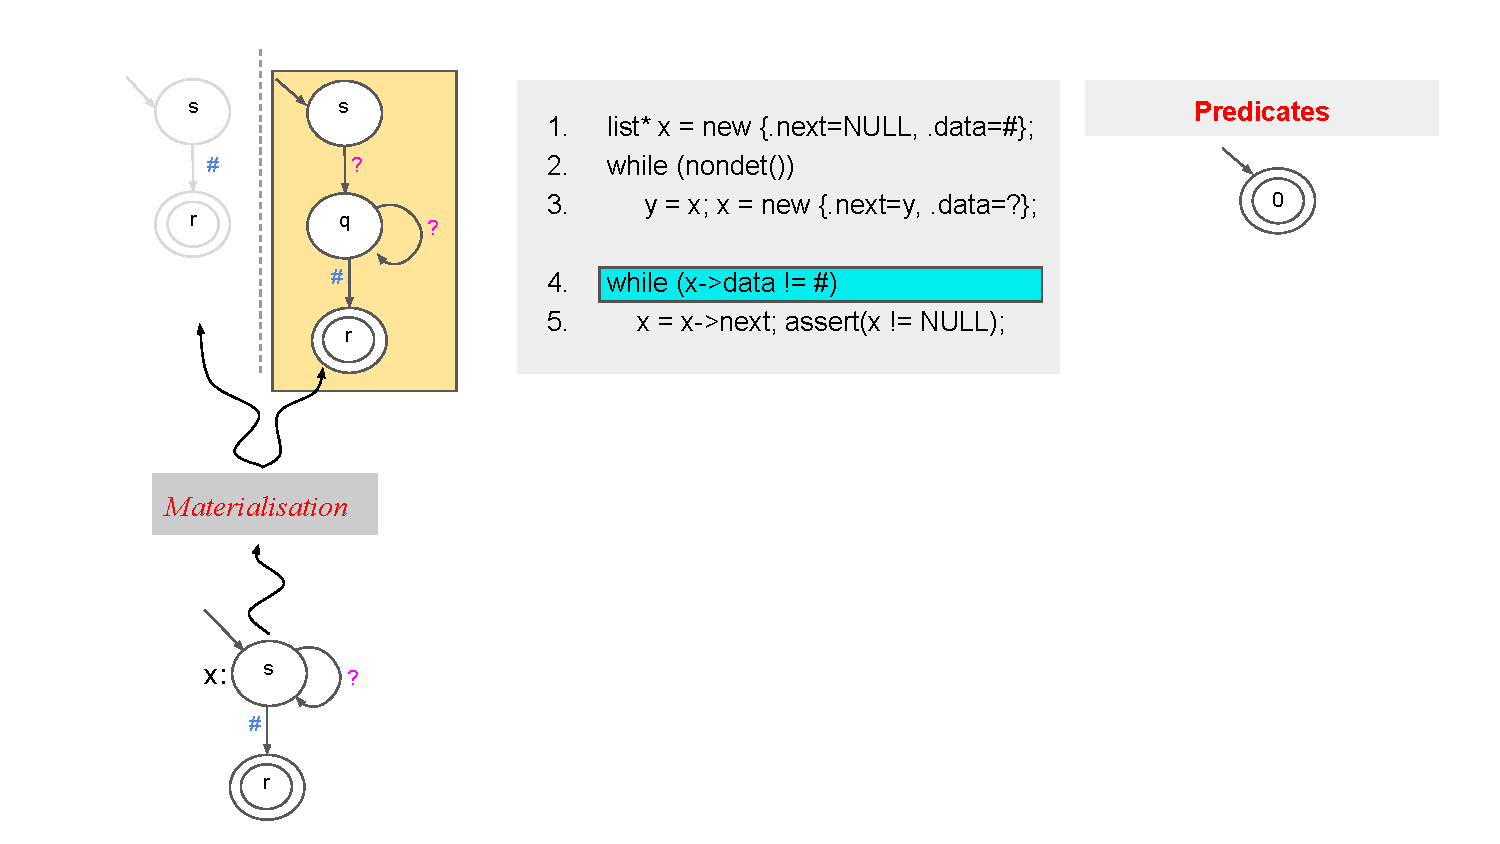
\includegraphics[scale=0.5]{ex/vmcai_23.pdf}}
       \only<12>{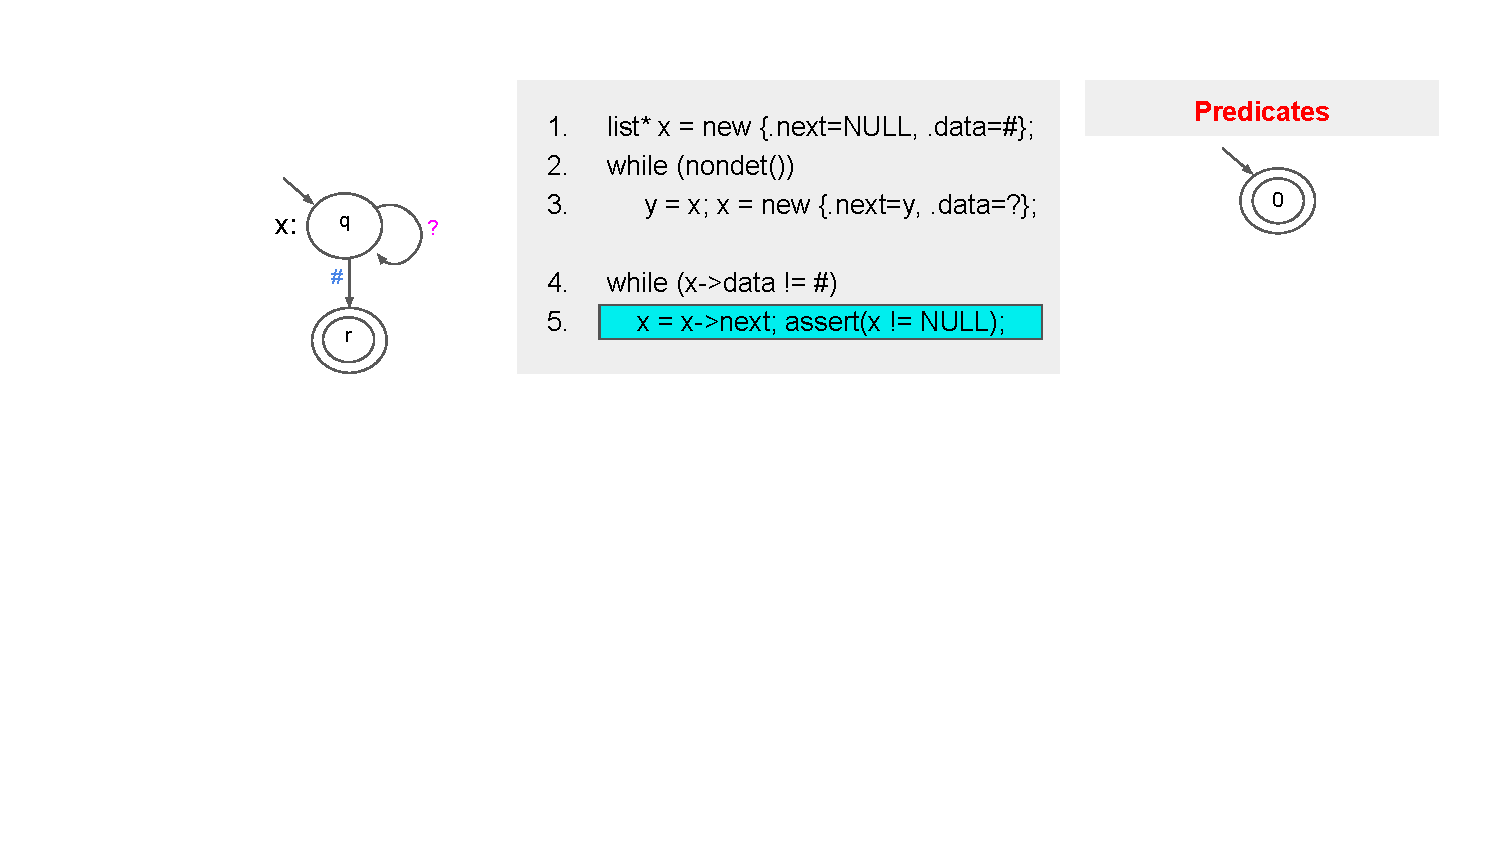
\includegraphics[scale=0.5]{ex/vmcai_24.pdf}}
       \only<13>{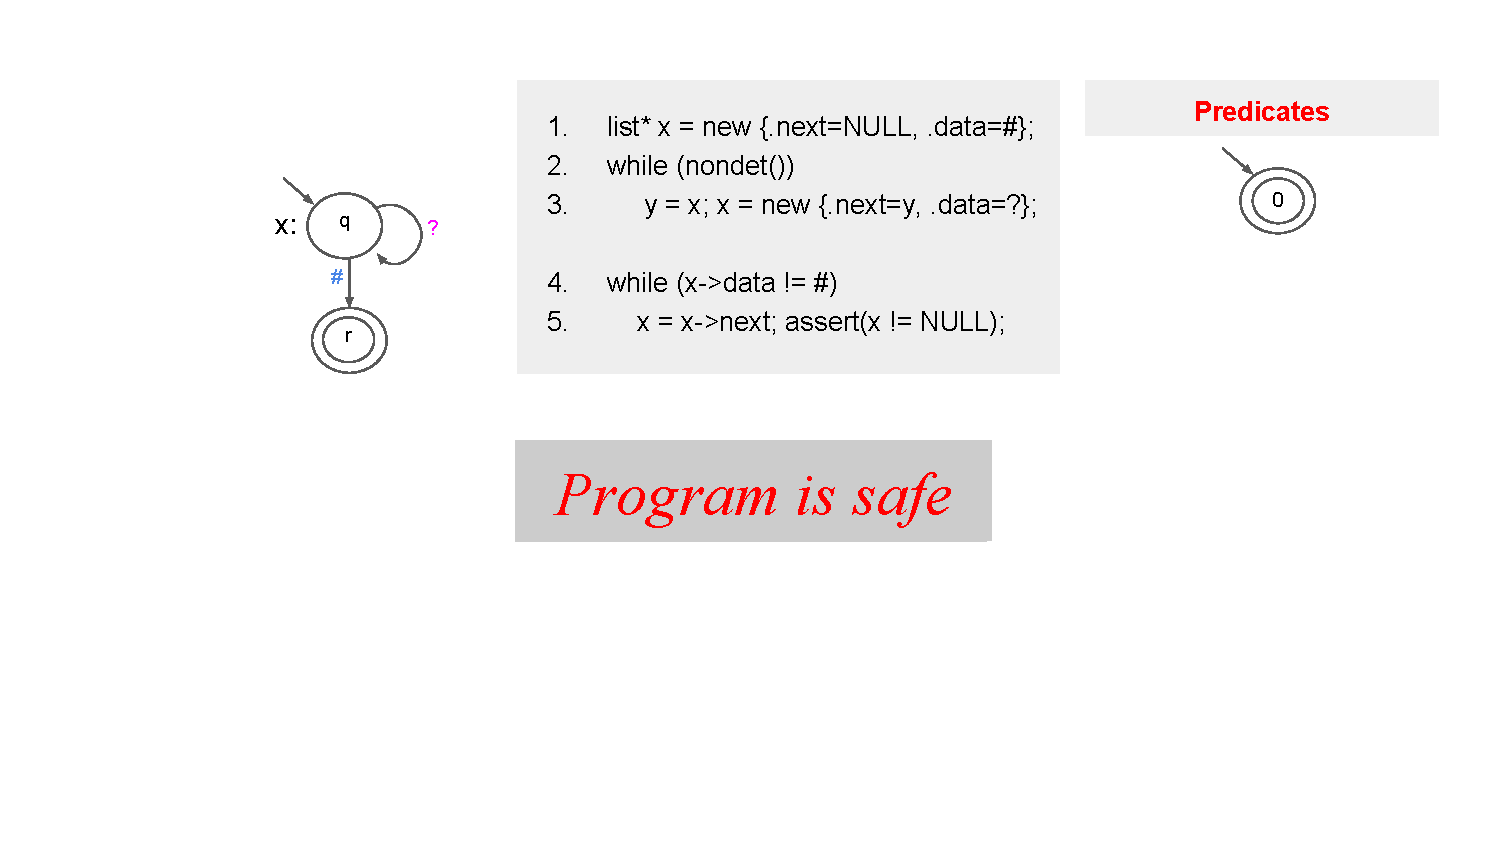
\includegraphics[scale=0.5]{ex/vmcai_25.pdf}}
     \end{overlayarea}
 \end{frame}
\end{comment}

%%*******************************************************************************

\end{document}
